\documentclass{article}

\usepackage{amsmath,geometry,amsfonts,array,makecell,enumitem,bm,esint,booktabs,multirow,mathtools,pgfplots,amssymb,nicematrix}
\usepackage[amsmath]{ntheorem}
\usepackage[hidelinks]{hyperref}
\usepackage[nameinlink,noabbrev]{cleveref}
\usepackage{ragged2e}
\usepackage{fancyhdr}
\pagestyle{fancy}
\fancyhead[L]{\itshape\nouppercase{\leftmark}}
\fancyhead[R]{IB Groups, Rings and Modules}

\title{Groups, Rings and Modules}
\author{Yue Wu}

\geometry{a4paper,hmargin=1.1in,vmargin=1.2in}

\setlength{\parskip}{1em}
\tolerance=1000
\emergencystretch=1em
\hyphenpenalty=1000
\exhyphenpenalty=100
\righthyphenmin=3

\theoremstyle{plain}\theoremheaderfont{\normalfont\itshape}\theorembodyfont{\rmfamily}\theoremseparator{.}\newtheorem*{rem}{Remark}\newtheorem*{ex}{Example}\newtheorem*{proof}{Proof}\newtheorem*{altp}{Alternative proof}\newtheorem*{nonex}{Non-Example}

\theoremstyle{plain}\theoremheaderfont{\normalfont\bfseries}\theorembodyfont{\rmfamily}\theoremseparator{.}\newtheorem{thm}{Theorem}[section]\newtheorem{lem}[thm]{Lemma}\newtheorem{prop}[thm]{Proposition}\newtheorem*{cor}{Corollary}\newtheorem{defn}[thm]{Definition}\newtheorem{clm}[thm]{Claim}\newtheorem{clminproof}{Claim}\newtheorem*{notn}{Notation}\newtheorem*{exer}{Exercise}\newtheorem*{lemnn}{Lemma}

\theoremstyle{break}\theoremheaderfont{\normalfont\itshape}\theorembodyfont{\rmfamily}\theoremseparator{.\medskip}\newtheorem*{proofskip}{Proof}\newtheorem*{exs}{Examples}\newtheorem*{rems}{Remarks}\newtheorem*{obs}{Observations}

\theoremstyle{break}\theoremheaderfont{\normalfont\bfseries}\theorembodyfont{\rmfamily}\theoremseparator{.\medskip}\newtheorem{lemskip}[thm]{Lemma}\newtheorem{defnskip}[thm]{Definition}\newtheorem{propskip}[thm]{Proposition}\newtheorem{thmskip}[thm]{Theorem}

\crefname{thm}{Theorem}{Theorems}\crefname{defn}{Definition}{Definitions}\crefname{lem}{Lemma}{Lemmas}\crefname{lemskip}{Lemma}{Lemmas}\crefname{cor}{Corollary}{Corollaries} \crefname{prop}{Proposition}{Propositions}\crefname{clm}{Claim}{Claims}

\numberwithin{equation}{section}
\setcounter{tocdepth}{2}

\usetikzlibrary{decorations.markings}

\NiceMatrixOptions{cell-space-limits = 2pt}

\newlength\ubwidth
\newcommand\parunderbrace[2]{\settowidth\ubwidth{$#1$}\underbrace{#1}_{\parbox{\ubwidth}{\scriptsize\RaggedRight#2}}}

\newcommand{\qed}{\hfill\ensuremath{\Box}}
\newcommand{\ii}{\mathrm{i}}
\newcommand{\ee}{\mathrm{e}}
\newcommand{\abs}[1]{\left|#1\right|}
\DeclareMathOperator*{\ord}{ord}
\DeclareMathOperator*{\im}{im}
\DeclareMathOperator*{\sign}{sign}
\DeclareMathOperator*{\Sym}{Sym}
\DeclareMathOperator*{\id}{id}
\DeclareMathOperator*{\Aut}{Aut}
\DeclareMathOperator{\Cl}{Cl}
\DeclareMathOperator{\Syl}{Syl}
\DeclareMathOperator{\GL}{GL}
\DeclareMathOperator{\SL}{SL}
\DeclareMathOperator{\lcm}{lcm}
\DeclareMathOperator{\Ann}{Ann}
\DeclareMathOperator{\Fit}{Fit}
\DeclareMathOperator{\adj}{adj}
\DeclareMathOperator{\diag}{diag}
\DeclareMathOperator{\tr}{tr}
\newcommand{\NN}{\mathbb{N}}
\newcommand{\ZZ}{\mathbb{Z}}
\newcommand{\QQ}{\mathbb{Q}}
\newcommand{\RR}{\mathbb{R}}
\newcommand{\CC}{\mathbb{C}}
\newcommand{\HH}{\mathbb{H}}
\newcommand{\FF}{\mathbb{F}}
\newcommand{\DD}{\mathbb{D}}
\newcommand{\MOD}[1]{\ (\mathrm{mod} \ #1)}
\newcommand{\biject}{\tikz[baseline=-1ex]{\node at (0,0){\(\longmapsto\)};\node at (0,-0.2){\reflectbox{\(\longmapsto\)}};}\,}
\newcommand{\longmappedfrom}{\;\reflectbox{\(\longmapsto\)}\;}
\newcommand{\mappedfrom}{\;\reflectbox{\(\mapsto\)}\;}

\pgfplotsset{compat=1.18}


\begin{document}
    \setlength{\parindent}{0pt}
	\Huge\textsf{\textbf{Groups, Rings and Modules}}
		
	\Large\textsf{\textbf{University of Cambridge Part IB Mathematical Tripos}}

	\noindent\makebox[\linewidth]{\rule{\textwidth}{2pt}}

	\large\textsf{\textbf{Yue Wu}}
	\begin{itemize}[topsep=0pt,leftmargin=15pt]
		\item[] \textit{Yusuf Hamied Department of Chemistry\\
		Lensfield Road,\\
		Cambridge, CB2 1EW}\\

		\textit{yw628@cam.ac.uk}
	\end{itemize}
    \thispagestyle{empty}
    \pagenumbering{roman}
    \setlength{\parindent}{15pt}
	
    \normalsize
    \newpage
	\tableofcontents
	\newpage
    \pagenumbering{arabic}

    \section{Groups}
    \subsection{Basic Concepts}
    \begin{defn}
        A \textit{group} is a triple \((G,\ \cdot \ , e)\) of a set \(G\), a function \(\ \cdot\ :G\times G\to G\) and an element \(e\in G\) such that
        \begin{itemize}[topsep=0pt,leftmargin=40pt]
            \item[(G1)] Associativity. \(\forall a,b,c\in G\), \(a\cdot(b\cdot c)=(a\cdot b)\cdot c\).
            \item[(G2)] Identity. \(\forall a\in G\), \(a\cdot e=e\cdot a=a\).
            \item[(G3)] Inverse. For each \(a\in G\), \(\exists a^{-1}\in G\) such that \(a\cdot a^{-1}=a^{-1}\cdot a=e\).  
        \end{itemize}
    \end{defn}
    \begin{defn}
        If \((G,\ \cdot \ ,e)\) is a group and \(H\subseteq G\) is a subset, then \(H\) is a \textit{subgroup} of \(G\), denoted \(H\le G\) if
        \begin{enumerate}[topsep=0pt,label=(\roman*)]
            \item If \(a,b\in H\), then \(a\cdot b\in H\).
            \item \(e\in H\).
            \item \((H, \ \cdot \ ,e)\) is a group.
        \end{enumerate}
    \end{defn}
    \begin{lem}
        \(\varnothing\ne H\subseteq G\) is a subgroup \(\iff\forall h_1,h_2\in H\), \(h_1\cdot h_2^{-1}\in H\).
    \end{lem}
    \begin{exs}
        \begin{enumerate}[topsep=0pt,label=(\roman*)]
            \item Additive groups. \((\ZZ,+,0),(\QQ,+,0),(\RR,+,0),(\CC,+,0)\)\dots
            \item Groups of symmetry.
            \begin{itemize}
                \item \(S_n\) symmetry groups \(=\) bijections of \(\{1,2,\dots,n\}\) to itself.
                \item \(D_{2n}\) dihedral group \(=\) symmetry of the regular \(n\)-gon.
                \item \(\GL_n(\RR)\) general linear group \(=\) symmetry of the vector space \(\RR^n\).
            \end{itemize}
            \item Subgroups of these.
            \begin{itemize}
                \item Alternating groups \(A_n\le S_n\), the even permutations.
                \item Cyclic groups \(C_n\le D_{2n}\), rotational symmetry of \(n\)-gon.
                \item Special linear groups \(\SL_n(\RR)\le\GL_n(\RR)\), \(\{A\in\GL_n(\RR)\mid\det{A}=1\}\).
            \end{itemize}
            \item Abelian groups \(G\) such that \(a\cdot b=b\cdot a\) \(\forall a,b\in G\), e.g. \(C_2\times C_2\cong V_4\).
            \item Quaternion group \(Q=\{\pm 1,\pm \ii,\pm \mathrm{j},\pm \mathrm{k}\}\).
        \end{enumerate}
    \end{exs}
    \begin{defn}
        For a subgroup, the \textit{left coset}
        \[gH\coloneqq\{x\in G\mid x=g\cdot h\text{ for some }h\in H\}\,.\]
        The collection of all left cosets of \(H\), written \(G:H\), gives a partition of \(G\). Each \(H\)-coset is in bijection with \(H\) (and also with each other).
    \end{defn}
    \begin{thm}[Lagrange's theorem]
        If \(G\) is a finite group and \(H\le G\), then
        \[\abs{G}=\abs{H}\abs{G:H}\,,\]
        where \(\abs{G:H}\) is the number of \(H\)-cosets in \(G\), known as the \textit{index} of \(H\) in \(G\).
    \end{thm}
    \begin{defn}
        The \textit{order} of \(g\in G\) is the least \(n\in\NN\cup\{\infty\}\) such that \(g^n=e\). Write \(\ord(g)\) for the number.
    \end{defn}
    If \(g^m=e\), then \(\ord(g)\mid m\).
    \begin{lem}
        Let \(G\) be a finite group. \(\ord(g)\mid\abs{G}\) \(\forall g\in G\).
    \end{lem}
    \begin{proof}
        If \(n=\ord(g)\), then \(H=\{e,g,g^2,\dots,g^{n-1}\}\). Claim that \(H\) is a subgroup of \(G\). If \(g^i,g^j\in H\), then \(g^i\cdot(g^j)^{-1}=g^{i-j}\), write \(i-j=p\cdot n+r\), with \(0\le r< n\).
        \[g^{i-j}=g^{pn+r}=(g^n)^p\cdot g^r=g^r\in H\,,\]
        so \(H\) is indeed a subgroup. By Lagrange's theorem, \(n=\abs{H}\) divides \(\abs{G}\).\qed
    \end{proof}
    \subsection{Normal Subgroups, Quotient, Homomorphism and Isomorphism}
    If \(gH=g'H\), then \(g^{-1}g'\in H\) and the converse holds. Let \(G/H\) be the set of the left \(H\)-cosets in \(G\), try to define
    \[(g_1H)\cdot(g_2H)=g_1g_2 H\,.\]
    This is well-defined only if the result is consistent for different choices of coset representatives. If \(g_2H=g_2hH\) is another coset representative, then
    \[(g_1H)\cdot(g_2hH)=g_1g_2hH=g_1g_2H\,.\]
    If \(g_1H=g_1hH\), then
    \[(g_1hH)\cdot(g_2H)=g_1hg_2H\,,\]
    which is equal to \(g_1g_2H\) if and only if
    \[(g_1g_2)^{-1}g_1hg_2=g_2^{-1}hg_2\in H\,.\]
    Hence this definition is legal if and only if \(g^{-1}hg\in H\) for all \(g\in G\), \(h\in H\).
    \begin{defn}
        A subgroup \(H\le G\) is \textit{normal}, denoted \(H\lhd G\), if
        \[g^{-1}hg\in H\]
        \(\forall h\in H, g\in G\).
    \end{defn}
    \begin{prop}
        If \(H\lhd G\), then the set \(G/H\) of left \(H\)-cosets form a group under the operation \((g_1H)\cdot(g_2H)=g_1g_2H\), with \(e_{G/H}=eH\). This is the \textit{quotient group} of \(G\) by \(H\).
    \end{prop}
    \begin{proof}
        The discussions show that this well-defines a binary operation on \(G/H\). All the axioms follow from the fact that they hold in \(G\).\qed
    \end{proof}
    \begin{defn}
        If \((G,\cdot_{G},e_G)\) and \((H,\cdot_{H},e_H)\) are groups, then a function \(\phi:G\to H\) is a \textit{homomorphism} if
        \begin{enumerate}[topsep=0pt,label=(\roman*)]
            \item \(\phi(g_1\cdot_G g_2)=\phi(g_1)\cdot_H \phi(g_2)\)
            \item \(\phi(e_G)=e_H\)
        \end{enumerate}
        The \textit{kernel} of \(\phi\) is \(\ker(\phi)\coloneqq\{g\in G\mid\phi(g)=e_H\}\), and the \textit{image} of \(\phi\) is \(\im(\phi)\coloneqq\{h\in H\mid h=\phi(g)\text{ for some }g\in G\}\).
    \end{defn}
    \begin{lem}
        If \(\phi:G\to H\) is a homomorphism, then \(\phi(g^{-1})=\phi(g)^{-1}\).
    \end{lem}
    \begin{proof}
        \begin{align*}
            \phi(g\cdot_G g^{-1})&=\phi(e_G)=e_H\\
            &=\phi(g)\cdot_H\phi(g)^{-1}\,.
        \end{align*}
        By the uniqueness of inverse, we must have \(\phi(g^{-1})=\phi(g)^{-1}\).\qed
    \end{proof}
    \begin{lem}
        For a homomorphism \(\phi:G\to H\), the kernel \(\ker(\phi)\) is a normal subgroup of \(G\), and the image \(\im(\phi)\) is a subgroup of \(H\).
    \end{lem}
    \begin{proof}
        Let \(g,h\in\ker(\phi)\), then
        \[\phi(g\cdot h^{-1})=\phi(g)*\phi(h)^{-1}=e_H*e_H^{-1}=e_H\,,\]
        so \(gh^{-1}\in\ker(\phi)\). Also \(\phi(e_G)=e_H\) so it is a subgroup. Let \(x\in G\), we have
        \begin{align*}
            \phi(x^{-1}gx)&=\phi(x^{-1})*\phi(g)*\phi(x)=\phi(x^{-1})*\phi(x)\\
            &=\phi(x^{-1}x)=\phi(e_G)=e_H\,,
        \end{align*}
        so \(x^{-1}gx\in\ker(\phi)\) and hence \(\ker\phi\) is normal.

        Let \(\phi(g),\phi(h)\in\im(\phi)\), then
        \[\phi(g)*\phi(h)^{-1}=\phi(gh^{-1})\in\im(\phi)\,.\]
        Furthermore, \(e_H=\phi(e_G)\in\im(\phi)\), so \(\im(\phi)\) is non-empty, and is a subgroup of \(H\).\qed
    \end{proof}
    \begin{defn}
        An \textit{isomorphism} is a homomorphism which is also a bijection.
    \end{defn}
    If a function \(\phi:G\to H\) is an isomorphism, then the inverse function \(\phi^{-1}:H\to G\) is too.
    \begin{defn}
        Two groups are \textit{isomorphic} if there is an isomorphism between them. We write \(G\cong H\).
    \end{defn}

    We often consider isomorphic groups to be ``the same'', and do not distinguish between them. We should be aware that we are careless when doing this.

    It is helpful to be able to break groups apart into smaller pieces. The following three isomorphism theorems allow us to do this in various ways. The first relates the kernel and image of an isomorphism.
    \begin{thm}
        Let \(\phi:G\to H\) be a homomorphism, then
        \[G/\ker(\phi)\cong\im(\phi)\,.\]
    \end{thm}
    \begin{proof}
        Let
        \begin{align*}
            f:G/\ker(\phi)&\longrightarrow\im(\phi)\\
            g\ker(\phi)&\longmapsto\phi(g)\,.
        \end{align*}
        First let us prove \(f\) is well-defined since it uses a coset representative. If \(g\ker(\phi)=g'\ker(\phi)\), then \(g^{-1}g'\in\ker(\phi)\) and so \(\phi(g^{-1}g')=e_H\). Thus
        \[e_{H}=\phi(g^{-1}g')=\phi(g^{-1})*\phi(g')\,,\]
        and so multiplying by \(\phi(g)\) gives \(\phi(g)=\phi(g')\), so the function is well-defined.

        \(f\) is a homomorphism since
        \begin{align*}
            f(g\ker(\phi)\cdot g'\ker(\phi))&=f(gg'\ker\phi)\\
            &=\phi(gg')\\
            &=\phi(g)*\phi(g')\\
            &=f(g\ker(\phi))*f(g'\ker(\phi))\,.
        \end{align*}
        Let \(h\in\im(\phi)\), then \(h=\phi(g)\) for some \(g\), so \(h=f(g\ker\phi)\) is in the image of \(f\). Therefore, \(f\) is surjective. Suppose that \(f(g\ker(\phi))=f(g'\ker(\phi))\), then \(\phi(g)=\phi(g')\), so \(\phi(g^{-1}g')=e_H\). Hence, \(g^{-1}g'\in\ker(\phi)\) and \(g\ker(\phi)=g'\ker(\phi)\), so \(f\) is injective. Therefore, \(f\) is an isomorphism.\qed
    \end{proof}
    \begin{ex}
        Consider the function \(\phi:\CC\to\CC\setminus\{0\}\) by \(z\mapsto \ee^z\). As \(\ee^{z+w}=\ee^z\cdot \ee^w\), \(\phi\) defines a homomorphism
        \[\phi:(\CC,+,0)\to (\CC\setminus\{0\},\times,1)\,.\]
        The existence of \(\log\) shows that \(\phi\) is surjective, and so \(\im(\phi)=\CC\setminus\{0\}\). The kernel is given by
        \[\ker\phi=\{z\in\CC\mid \ee^z=1\}=2\pi \ii\ZZ\,.\]
        The conclusion is that
        \[(\CC/(2\pi \ii\ZZ),+,0)\cong(\CC\setminus\{0\},\times,1)\,.\]
    \end{ex}
    \begin{thm}[Second isomorphism theorem]
        Let \(H\le G\) and \(K\lhd G\). Then \(HK\coloneqq\{h\cdot k\mid h\in H,k\in K\}\) is a subgroup of \(G\), and \(H\cap K\) is a normal subgroup of \(G\). Moreover,
        \[\frac{HK}{K}\cong\frac{H}{H\cap K}\,.\]
    \end{thm}
    \begin{proof}
        Let \(hk,h'k'\in HK\), then
        \[h'k'(hk)^{-1}=h'k'k^{-1}h^{-1}=(h'h^{-1})(hk'k^{-1}h^{-1})\,.\]
        The first term is in \(H\), and the second term is \(k'k^{-1}\in K\) conjugated by \(h\), which is also in \(K\). Therefore, \(h'k'(hk)^{-1}\) lies in \(HK\), and \(HK\) also contains \(e_G\), so it is a subgroup.

        Define
        \begin{align*}
            \phi:H&\longrightarrow G/K\\
            h&\longmapsto hK\,.
        \end{align*}
        This is a homomorphism. The image of \(\phi\) is the set of \(K\)-cosets which may be represented by an element of \(H\), i.e.
        \[\im(\phi)=\frac{HK}{K}\,.\]
        The kernel of \(\phi\) is
        \[\ker(\phi)=\{h\in H\mid hK=eK\}=\{h\in H\mid h\in K\}=H\cap K\,.\]
        As \(H\cap K\) is the kernel of a homomorphism, it is normal in \(H\). By the first isomorphism theorem,
        \[\frac{H}{H\cap K}\cong\frac{HK}{K}\,.\]
    \end{proof}

    Note that if \(K\lhd G\), then there is a bijection between subgroups of \(G/K\) and subgroups of \(G\) containing \(K\), given by
    \begin{align*}
        \{\text{subgroups of }G/K\}&\longleftrightarrow\{\text{subgroups of }G\text{ which contains }K\}\\
        X\le\frac{G}{K}&\longmapsto\{g\in G\mid gK\in X\}\\
        \frac{L}{K}\le\frac{G}{K}&\longmappedfrom K\lhd L\le G\,.
    \end{align*}
    This specialises to a bijection between normal subgroups as well.
    \[\{\text{normal subgroups of }G/K\}\longleftrightarrow\{\text{normal subgroups of }G\text{ which contains }K\}\,.\]
    \begin{thm}[Third isomorphism theorem]
        Let \(K\le L\le G\) be normal subgroups of \(G\), then
        \[\frac{G/K}{L/K}\cong\frac{G}{L}\,.\]
    \end{thm}
    \begin{proof}
        Let
        \begin{align*}
            \phi:G/K&\longrightarrow G/L\\
            gK&\longmapsto gL\,.
        \end{align*}
        If \(gK=g'K\), then \(g^{-1}g'\in K\in L\) so \(gL=g'L\), so well-defined. It is a homomorphism, and onto.
        \begin{align*}
            \ker(\phi)=\{gK\in G/K\mid gL&=eL\}=L/K\,,\\
            &\Updownarrow\\
            g&\in L
        \end{align*}
        so done by \(1^{\text{st}}\) isomorphism theorem.\qed
    \end{proof}
    \begin{defn}
        A non-trivial group \(G\) is \textit{simple} if its only normal subgroups are \(\{e\}\) or \(G\).
    \end{defn}
    \begin{lem}
        An abelian group is simple \(\iff\) it is \(C_p\) for some prime number \(p\).
    \end{lem}
    \begin{proofskip}
        \begin{enumerate}[topsep=0pt]
            \item[(\(\Leftarrow\))] If \(H\le C_p\), then \(\abs{H}\mid\abs{C_p}=p\) by Lagrange's theorem, so \(\abs{H}=1\) or \(p\), so \(H=\{e\}\) or \(C_p\).
            \item[(\(\Rightarrow\))] Let \(G\) be a simple abelian group. All subgroups of \(G\) are normal since
            \[g^{-1}hg=g^{-1}gh=h\ \forall h\in H\lhd G\,.\]
            Let \(e\ne g\in G\), and \(H=\{\dots,e,g,g^2,\dots\}\) is a normal subgroup. As \(g\ne e\), \(H\ne\{e\}\) so \(H=G\) as \(G\) is simple, so \(G\) is cyclic. Then \(G\cong (\ZZ,+,0)\) or \(G\cong C_n\). But \(2\ZZ\lhd\ZZ\), so \(\ZZ\) is not simple. If \(m\mid n\), then \(g^{n/m}\) generates a subgroup of \(C_n\) of order \(m\), and it is normal. Therefore for \(C_n\) to be simple, only \(1\) and \(n\) can divide \(n\).\qed
        \end{enumerate}
    \end{proofskip}
    \begin{thm}
        If \(G\) is a finite group, then there are subgroups
        \[G=H_1>H_2>\dots>H_s=\{e\}\,.\]
    \end{thm}
    \begin{proof}
        If \(G\) is simple, let \(H_2=\{e\}\) and done.

        If not, let \(H_2\lhd G\) be a proper normal subgroup of the largest order among all proper normal subgroups. Then claim \(G/H_2\) is simple: if not, it has a proper \(K\lhd G/H_2\). However, by the correspondence between normal subgroups of \(G/H_2\) and normal subgroups of \(G\) containing \(H_2\), \(K\cong L/H_2\) for some \(L\lhd G\) such that \(H_2\lhd L\). We find a proper normal subgroup of \(G\) with order strictly large than \(H_2\), so contradiction.

        So we found an \(H_2\lhd G\) with \(G/H_2\) simple. Repeat this process to get the required sequence of normal subgroups. This process eventually stops as \(\abs{G}\) is finite.\qed
    \end{proof}
    \subsection{Actions and Permutations}
    Recall \textit{permutation groups}
    \begin{align*}
        S_n&\coloneqq\text{symmetry group on }\{1,2,\dots,n\}\\
        &\equiv\text{group of bijections from }\{1,2,\dots,n\}\text{ to itself.}
    \end{align*}
    Can define the \textit{sign} function on \(S_n\)
    \begin{align*}
        \sign:S_n&\longrightarrow(\{\pm 1\},\times,+1)\\
        \sigma&\longmapsto\begin{cases}
            +1 & \sigma=\text{even \# permutations}\\
            -1 & \sigma=\text{odd \# permutations.}
        \end{cases}
    \end{align*}
    It is a homomorphism, so \(S_n\) has a normal subgroup
    \[A_n\coloneqq\ker(\sign)\lhd S_n\]
    called the \textit{alternating group}, and it has an index \(2\). More generally, for a set \(X\), the \textit{symmetry group} is
    \[\Sym(X)\coloneqq\{\sigma:X\to X\mid\sigma\text{ is a bijection}\}\,.\]
    \begin{defn}
        A group is a \textit{permutation group} on \(X\) if it is a subgroup of \(\Sym(X)\). Say it is a permutation group of \textit{degree} \(n\) if \(\abs{X}=n\).
    \end{defn}
    \begin{exs}
        \begin{enumerate}[topsep=0pt,label=(\roman*)]
            \item \(S_n=\Sym(\{1,2,\dots,n\})\) is a permutation group of degree \(n\).
            \item \(D_{2n}=\Sym(\text{vertices of a regular }n\text{-gon})\).
        \end{enumerate}
    \end{exs}
    \begin{defn}
        An \textit{action} of a group \(G\) on a set \(X\) is a function
        \[-*-:G\times X\to X\]
        such that
        \begin{enumerate}[topsep=0pt,label=(\roman*)]
            \item \(\forall x\in X, g_i\in G\), \(g_1*(g_2*x)=(g_1g_2)*x\)
            \item \(\forall x\in X\), \(e*x=x\).
        \end{enumerate}
    \end{defn}
    \begin{lem}
        An action \(G\) on \(X\) is the same as a homomorphism \(\phi:G\to\Sym(X)\).
    \end{lem}
    \begin{proof}
        Let \(-*-:G\times X\to X\) be a function. Define \(\phi(g)=g*-:X\to X\) be a function. Note
        \begin{align*}
            \phi(g^{-1})\circ\phi(g)(x)&=g^{-1}*(g*x)\\
            &=(g^{-1}g)*x\\
            &=x
        \end{align*}
        \(\forall x\), so \(\phi(g^{-1})\) is inverse to \(\phi(g)\), so \(\phi(g)\) is a bijection. This defines a function \(\phi:G\to\Sym(X)\). Note
        \[(\phi(h)\circ\phi(g))(x)=\phi(hg)(x)\ \forall x\in X, h,g\in G\,,\]
        so \(\phi\) is a homomorphism.

        Conversely, let \(\phi:G\to\Sym(X)\) be a homomorphism. Let \(g*x=\phi(g)(x)\), then
        \begin{align*}
            g*(h*x)&=\phi(g)(\phi(h)(x))\\
            &=(\phi(g)\circ\phi(h))(x)\\
            &=\phi(gh)(x)\\
            &=(gh)*x\,,
        \end{align*}
        so it defines a group action.\qed
    \end{proof}
    \begin{defn}
        A permutation representation of a group \(G\) is a homomorphism \(G\to\Sym(X)\).
    \end{defn}
    The lemma above has shown that a permutation representation is the same as a group action. The good thing about thinking of group actions as homomorphisms is that we can use all we know about homomorphisms on them.
    \begin{defn}
        For an action of \(G\) on \(X\), we write
        \begin{align*}
            G^X&\coloneqq\im(\phi:G\to\Sym(X))\\
            G_X&\coloneqq\ker(\phi:G\to\Sym(X))\,.
        \end{align*}
    \end{defn}
    \begin{prop}
        \(G^X\cong G/G_X\).
    \end{prop}
    \begin{proof}
        \(1^{\text{st}}\) isomorphism theorem.\qed
    \end{proof}
    \begin{exs}
        \begin{enumerate}[topsep=0pt,label=(\roman*)]
            \item
            \begin{align*}
                G&=\text{symmetries of the cube}\\
                X&=\{\text{diagonals of the cube}\}\\
                G^X&=\Sym(X)\cong S_4\\
                G_X&=\{\id,\text{ sending each vertex to its opposite}\}\,.
            \end{align*}
            \begin{figure}[ht!]
                \centering
                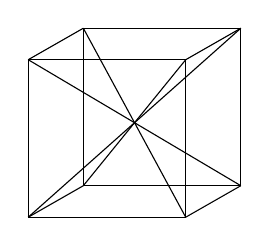
\begin{tikzpicture}
                    \draw (0,0) rectangle (2,2);
                    \draw (0.7,0.4) rectangle (2.7,2.4);
                    \draw (0,0)--(0.7,0.4);
                    \draw (2,0)--(2.7,0.4);
                    \draw (0,2)--(0.7,2.4);
                    \draw (2,2)--(2.7,2.4);
                    \draw (0,0)--(2.7,2.4);
                    \draw (2,0)--(0.7,2.4);
                    \draw (0.7,0.4)--(2,2);
                    \draw (2.7,0.4)--(0,2);
                \end{tikzpicture}
            \end{figure}
            Have \(\abs{G^X}=4!=24\) and \(\abs{G_X}=2\), so \(\abs{G}=48\).
            \item The group \(G\) acts on itself via \(g*g'=g\cdot g'\). This corresponds to a \(\phi:G\to\Sym(G)\).
            \[G_X=\{g\in G\mid g*g'=g'\ \forall g'\in G\}=\{e\}\,,\]
            so \(G=G/\{e\}\cong C^X\le\Sym(G)\). This gives the Cayley's theorem. Every group is (isomorphic to) a subgroup of a symmetric group.
            \item For \(H\subseteq G\). Let \(X=G/H\) set of left \(H\)-cosets. \(G\) acts on \(X=G/H\) via \(g*g'H=(gg')H\). This is well defined so we get \(\phi:G\to\Sym(X)\).
            
            Now consider \(G_X=\ker(\phi)\). If \(g\in G_X\), then for every \(g_1\in G\), we have \(g*g_1H=g_1H\). This means \(g_1^{-1}gg_1\in H\). In other words, we have \(g\in g_1Hg_1^{-1}\). This has to hold for all \(g_1\in G\), so
            \[G_X\subseteq\bigcap_{g_1\in G}g_1Hg_1^{-1}\,.\]

            This argument is completely reversible: if \(g\in\bigcap_{g_1\in G}g_1Hg_1^{-1}\), then for each \(g_1\in G\), we know that \(g_1^{-1}gg_1\in H\) and hence \(gg_1H=g_1H\). So \(g*g_1H=g_1H\) and hence \(g\in G_X\). Thus we have
            \[\ker(\phi)=G_X=\bigcap_{g_1\in G}g_1Hg_1^{-1}\,.\]
            Since this is a kernel, it is a normal subgroup of \(G\), and is contained in \(H\). Starting with an arbitrary subgroup \(H\), this allows us to generate a normal subgroup. (If we think about the construction, we see that this is the largest normal subgroup of \(G\) that is contained in \(H\).)
        \end{enumerate}
    \end{exs}
    \begin{thm}
        Let \(G\) be a finite group, \(H\le G\) be a subgroup of index \(n\). Then there is a \(K\lhd G\) with \(K\le H\) such that \(\abs{G/K}\mid n!\) and \(n\mid\abs{G/K}\).
    \end{thm}
    \begin{proof}
        We apply the previous example. Act by \(G\) on \(G/H\), set \(K=G_X\lhd G\). Then \(G/G_X\cong G^X\le\Sym(G/H)\cong S_n\,,\)
        so by Lagrange's theorem, \(\abs{G/K}\mid\abs{S_n}=n!\). We also have \(K\le H\), so \(\abs{G/K}\ge\abs{G:H}=n\).\qed
    \end{proof}
    \begin{cor}
        Let \(G\) be a non-abelian simple group, and \(H\) a proper subgroup of index \(n>1\). Then \(G\) is isomorphic to a subgroup of \(A_n\), with \(n\ge 5\).
    \end{cor}
    \begin{proof}
        Act by \(G\) on the set \(G/H\) gives a homomorphism \(\phi:G\to\Sym(G/H)\). Then \(G_X\lhd G\) is normal, so as \(G\) is simple, \(G_X=\{e\}\) or \(G_X=G\). As \(g*(eH)\ne eH\) for \(g\notin H\), which exists since the subgroup \(H\) is proper, the kernel of this action is not \(G\), so \(G_X=\{e\}\). Therefore, \(\phi\) is injective, so \(G=G/G_X\cong G^X\le\Sym(G/H)\cong S_n\).
        
        Now \(A_n\lhd S_n\), so \(G\cap A_n\lhd G\), so as \(G\) is simple, \(G\cap A_n=\{e\}\) or \(G\cap A_n=G\). If \(G\cap A_n=\{e\}\), then
        \[G=\frac{G}{G\cap A_n}\cong\frac{G\cdot A_n}{A_n}\le\frac{S_n}{A_n}\cong C_2\]
        by the second isomorphism theorem. Hence, \(\abs{G}\le 2\). This is a contradiction as \(G\) is non-abelian. Therefore, we have
        \[G\cap A_n=G\implies G\le A_n\,.\]
        \(A_1,A_2,A_3,A_4\) have no non-abelian simple subgroups.\qed
    \end{proof}
    \begin{defn}
        Let \(G\) act on \(X\). The \textit{orbit} of \(x\in X\) is
        \[G\cdot x\coloneqq\{x'\in X\mid x'=g*x\text{ for some }g\in G\}\,.\]

        The \textit{stabiliser} of \(x\in X\) is
        \[G_x\coloneqq\{g\in G\mid g*x=x\}\,.\]
    \end{defn}
    \begin{lem}
        \(G_x\) is a subgroup of \(G\).
    \end{lem}
    \begin{proof}
        \(e(x)=x\) by definition. For \(g,h\in G_x\), \(gh^{-1}(x)=g(h^{-1}*(x))=g(x)=x\).\qed
    \end{proof}
    \begin{lem}
        The orbits of an action partition \(X\).
    \end{lem}
    \begin{proof}
        \(\forall x\in X\), \(x\in G\cdot x\) as \(e*x=x\). So every \(x\) is in some orbit.
        
        Then suppose \(z\in G\cdot x\) and \(z\in G\cdot y\), we have to show that \(G\cdot x=G\cdot y\). We know that \(z=g_1*x=g_2*y\) for some \(g_1,g_2\in G\), so \(y=(g_2^{-1}g_1)*x\). For any \(w=g_3(y)\in G\cdot y\), we have \(w=(g_3g_2^{-1}g_1)*x\), so \(w\) is also in \(G\cdot x\). Thus \(G\cdot y\subseteq G\cdot x\) and similarly \(G\cdot x\subseteq G\cdot y\), so \(G\cdot x=G\cdot y\).\qed
    \end{proof}
    Let \(g\in G\), \(x\in X\). Each \(g\in G\) gives us a member \(g*x\in G\cdot x\), and conversely, every object in \(G\cdot x\) arises this way. However, different elements in \(G\) can give us the same orbit. In particular, if \(g\in G_x\), then \(hg\) and \(h\) give us the same object in \(G\cdot x\). So we have a correspondence between things in \(G\cdot x\) and members of \(G\), up to \(G_x\).
    \begin{thm}[Orbit-stabiliser theorem]
        Let \(G\) act on \(X\). Then for any \(x\in X\), there is a bijection
        \begin{align*}
            \phi:G\cdot x&\longleftrightarrow G:G_x\\
            g*x&\biject gG_x\,,
        \end{align*}
        and in particular, if \(G\) is finite, then \(\abs{G\cdot x}=\abs{G:G_x}\). 
    \end{thm}
    \begin{proof}
        \(\phi\) is well-defined since if \(g\cdot G_x=h\cdot G_x\), then \(h=gk\) for some \(k\in G_x\), so \(h*x=g*(k*x)=g*x\).
        
        This map is injective because if \(gG_x=hG_x\), then \(G_x=g^{-1}hG_x\) so \(g^{-1}h\in G_x\), then \(g^{-1}h*x=x\implies g*x=h*x\), and this map is clearly surjective. The rest follows from Lagrange's theorem.\qed
    \end{proof}
    \subsection{Conjugacy Classes, Centralisers, Normalisers}
    Can define an action of \(G\) on the set \(G\) via
    \[g*h=ghg^{-1}\,.\]
    The function \(\phi(g):G\to G\) satisfies
    \begin{align*}
        \phi(g)(ab)&=gabg^{-1}=(gag^{-1})(gbg^{-1})\\
        &=\phi(a)\phi(b)\,,
    \end{align*}
    so \(\phi(g)\) is a homomorphism. It is also a bijection, with inverse \(\phi(g^{-1})\). We can take the collection of all isomorphisms of \(G\), and form a new group out of it.
    \begin{defn}
        The \textit{automorphism group} of a group \(G\) is
        \[\Aut(G)\coloneqq\{f\in\Sym(G)\mid f\text{ is a group isomorphism}\}\,.\]
        This is a group under composition, with the identity map as the identity element.
    \end{defn}
    It is a subgroup of \(\Sym(G)\).
    \begin{defn}
        The \textit{conjugacy class} of \(g\in G\) is
        \[\Cl_G(g)\coloneqq G\cdot g=\{h\in G\mid h=xgx^{-1}, x\in G\}\,.\]

        The \textit{centraliser} of \(g\in G\) is
        \[C_G(g)\coloneqq G_g=\{x\in G\mid xgx^{-1}=g\}\,,\]
        i.e. the set of all \(x\in G\) which commute with \(g\).

        The \textit{centre} of \(G\) is
        \[Z(G)\coloneqq\ker(\phi)=\{x\in G\mid xgx^{-1}=g\ \forall g\in G\}=\bigcap_{g\in G}C_G(g)\,,\]
        i.e. the set of all \(x\in G\) which commute with all \(g\in G\).
    \end{defn}
    \begin{prop}
        \[\abs{\Cl_G(x)}=\abs{G:C_G(x)}=\frac{\abs{G}}{\abs{C_G(x)}}\,.\]
    \end{prop}
    \begin{proof}
        Orbit-stabiliser.\qed
    \end{proof}
    \begin{defn}
        The \textit{normaliser} of \(H\le G\) is
        \[N_G(H)\coloneqq\{g\in G\mid gHg^{-1}=H\}\,,\]
        i.e. the largest subgroup of \(G\) inside which \(H\) is normal.
    \end{defn}
    \begin{thm}
        \(A_n\) is simple for all \(n\ge 5\).
    \end{thm}
    \begin{proofskip}
        \begin{itemize}[topsep=0pt,parsep=1em,rightmargin=20pt]
            \item \begin{clminproof}
                \(A_n\) is generated by 3-cycles.
            \end{clminproof}
        \begin{proof}
                Every element of \(A_n\) is a product of evenly-many transpositions, so need to show that the product of two transpositions can be written in terms of 3-cycles.

                Let \(a,b,c,d\) be distinct.
                \begin{itemize}[topsep=0pt]
                    \item \((a \ b)(a \ b)=e\).
                    \item \((a \ b)(b \ c)=(a \ b \ c)\)
                    \item \((a \ b)(c \ d)=(a \ c \ b)(a \ c \ d)\).\qed
                \end{itemize}
            \end{proof}
            \item \begin{clminproof}
                If \(H\lhd A_n\) contains a 3-cycle, then it is \(A_n\).
            \end{clminproof}
        \begin{proof}
                We will show that if \(H\) contains a 3-cycle, it contains every 3-cycle, then done since \(A_n\) is generated by 3-cycles. Suppose \((a \ b \ c)\in H\) and want to show that \((1 \ 2 \ 3)\in H\). Since they have the same cycle shape, there is some \(\sigma\in S_n\) such that \((a \ b \ c)=\sigma^{-1}(1 \ 2 \ 3)\sigma\).
                
                If \(\sigma\) is even, then \(\sigma\in A_n\), so since \(H\lhd A_n\), we have \((1 \ 2 \ 3)\in H\) and done. If \(\sigma\) is odd, take \(\overline{\sigma}=\sigma(4 \ 5)\in A_n\) (here comes the condition \(n\ge 5\)), then \(\sigma^{-1}(1 \ 2 \ 3)\sigma=\overline{\sigma}^{-1}(1 \ 2 \ 3)\overline{\sigma}=(a \ b \ c)\) so done.\qed
            \end{proof}
        \end{itemize}

        Let \(H\lhd A_n\). We want to show that \(H\) contains a 3-cycle, so it is \(A_n\) itself. We split into different cases.
        \begin{enumerate}[topsep=0pt,label=(\roman*),parsep=1em,rightmargin=20pt]
            \item \begin{clminproof}
                If \(H\) contains a \(\sigma\) which can be written as
                \[\sigma=(1 \ 2 \ 3 \ dots \ r)\cdot\tau\]
                for \(r\ge 4\) and \(\tau\) arbitrary, then \(H\) contains a 3-cycle.
            \end{clminproof}
        \begin{proof}
                Let \(\delta=(1 \ 2 \ 3)\) and consider
                \begin{align*}
                    \underbrace{\underbrace{\sigma^{-1}}_{\in H}\cdot\underbrace{\delta^{-1}\cdot\sigma\cdot\delta}_{\in H}}_{\in H}&=(r \ \dots \ 2 \ 1)(1 \ 3 \ 2)(1 \ 2 \ \dots \ r)(1 \ 2 \ 3)\\
                    &=(2 \ 3 \ r)\,,
                \end{align*}
                where we used the assumption that \((1 \ 2 \ \dots \ r)\tau\) are disjoint so \(\tau\) commute with \((1 \ 2 \ \dots \ r)\) and \(\delta\).\qed
            \end{proof}
            \item \begin{clminproof}
                If \(H\) contains a \(\sigma=(1 \ 2 \ 3)(4 \ 5 \ 6)\cdot\tau\) disjoint, then it contains a 3-cycle.
            \end{clminproof}
        \begin{proof}
                Let \(\delta=(1 \ 2 \ 4)\). Then
                \begin{align*}
                    \sigma^{-1}\delta^{-1}\sigma\delta&=(1 \ 3 \ 2)(4 \ 6 \ 5)(1 \ 4 \ 2)(1 \ 3 \ 2)(4 \ 5 \ 6)(1 \ 2 \ 4)\\
                    &=(1 \ 2 \ 4 \ 3 \ 6)\in H\,.
                \end{align*}
                This is a 5-cycle, so the previous case applies.\qed
            \end{proof}
            \item \begin{clminproof}
                If \(H\) contains a \(\sigma=(1 \ 2 \ 3)\cdot\tau\) disjoint, then it contains a 3-cycle.
            \end{clminproof}
        \begin{proof}
                If \(\tau\) is a product of 2-cycles, then
                \[\sigma^2=(1 \ 2 \ 3)^2=(1 \ 3 \ 2)\]
                is a three cycle. If \(\tau\) is anything longer, then it falls into one of the previous cases.\qed
            \end{proof}
            \item \begin{clminproof}
                If \(H\) contains \(\sigma=(1 \ 2)(3 \ 4)\tau\) disjoint, then it contains a 3-cycle.
            \end{clminproof}
        \begin{proof}
                If \(\tau\) is a product of 2-cycles, let \(\delta=(1 \ 2 \ 3)\) then
                \begin{align*}
                    u&=\sigma^{-1}\delta^{-1}\sigma\delta\\
                    &=(1 \ 2)(3 \ 4)(1 \ 3 \ 2)(1 \ 2)(3 \ 4)(1 \ 2 \ 3)\\
                    &=(1 \ 4)(2 \ 3)\in H\,.
                \end{align*}
                Then let
                \[v=(1 \ 5 \ 2)u(1 \ 2 \ 5)=(1 \ 3)(4 \ 5)\in H\,,\]
                where we used \(n\ge 5\) again. Consider
                \[uv=(1 \ 4)(2 \ 3)(1 \ 3)(4 \ 5)=(1 \ 2 \ 3 \ 4 \ 5)\in H\,.\]
                This is the first case so done.

                If \(\tau\) is longer, it fits in one of the previous cases.\qed
            \end{proof}
        \end{enumerate}
        Combining these results, we are done.\qed
    \end{proofskip}
    \subsection{Finite \texorpdfstring{\(\bm{p}\)}{p}-groups.}
    We never seem to talk about things like the sum of orders of two subgroups. From this point of view, the simplest groups are those of prime orders, but they are all cyclic. The next simplest groups are those whose order is a power of prime.
    \begin{defn}
        A finite group is a \(p\)-group if \(\abs{G}=p^n\) for some prime number \(p\) and \(n\ge 1\).
    \end{defn}
    \begin{thm}
        If \(G\) is a finite \(p\)-group, then its centre \(Z(G)=\{x\in G\mid xg=gx \ \forall g\in G\}\) is non-trivial.
    \end{thm}
    \begin{proof}
        Let \(G\) act on itself by conjugation. Each orbit of this action (which are precisely the conjugacy classes) has size dividing \(\abs{G}=p^n\), so is either a singleton, or has size divisible by \(p\).

        Since the conjugacy classes partition \(G\), the sum of the sizes of the conjugacy classes is \(\abs{G}\). In particular,
        \[\abs{G}=\#\{\text{conjugacy classes of size }1\}+\sum\text{orders of all other conjugacy classes}\,.\]
        By the above discussion, the second term is divisible by \(p\), as is \(\abs{G}=p^n\). Therefore, the number of conjugacy classes of size 1 is divisible by \(p\). \(\{e\}\) is a conjugacy class of size \(1\), so \(\#\{\text{conjugacy classes of size }1\}\ge p\ge 2\). There must be a conjugacy class \(\{x\}\ne\{e\}\).

        Then, \(g^{-1}xg=x\) \(\forall g\in G\), i.e. \(x\in Z(G)\), so \(Z(G)\) is non-trivial.\qed
    \end{proof}
    \begin{cor}
        Let \(G\) be a \(p\)-group of order \(p^n\), \(n\ge 2\). \(G\) is not simple.
    \end{cor}
    \begin{proof}
        \(Z(G)\lhd G\).\qed
    \end{proof}

    This allows us to prove interesting things about \(p\)-groups by induction on their orders, by considering the smaller \(p\)-group \(G/Z(G)\). One way to do this is via the following lemma.
    \begin{lem}
        For any group \(G\), if \(G/Z(G)\) is cyclic, then \(G\) is abelian.
    \end{lem}
    In other words, if \(G/Z(G)\) is cyclic, then it is trivial, since the centre of an abelian group is the abelian group itself.
    \begin{proof}
        Let the coset \(gZ(G)\) be a generator of the cyclic group \(G/Z(G)\), so every coset of \(Z(G)\) is of the form \(g^rZ(G)\). It follows that every element \(x\in G\) must be in the form \(g^rz\) for some \(z\in Z(G)\), \(r\in\ZZ\).

        To show that \(G\) is abelian, let \(x'=g^{r'}z'\) another element in \(G\) with some \(z'\in Z(G)\) and \(r'\in\ZZ\). As \(z,z'\in Z(G)\), they commute with every element in \(G\), so
        \[xx'=g^rzg^{r'}z'=g^{r'}g^rz'z=g^{r'}z'g^rz=x'x\,,\]
        and hence \(G\) is abelian.\qed
    \end{proof}
    This lemma is particularly useful when applied to \(p\)-groups.
    \begin{cor}
        If \(p\) is prime and \(\abs{G}=p^2\), then \(G\) is abelian.
    \end{cor}
    \begin{proof}
        Since \(Z(G)\le G\), its order must be 1, \(p\) or \(p^2\). \(Z(G)\) is non-trivial, so \(\abs{Z(G)}=p\) or \(p^2\). If \(\abs{Z(G)}=p^2\), it is the whole group so \(G\) is trivially abelian. Otherwise, \(\abs{G/Z(G)}=p^2/p=p\) must be cyclic, so it must be cyclic, then \(G\) is again abelian.\qed
    \end{proof}
    \begin{thm}
        Let \(G\) be a group of order \(p^a\), where \(p\) is prime. Then \(G\) has a subgroup of order \(p^b\) for any \(0\le b\le a\).
    \end{thm}
    \begin{rem}
        This means that \(G\) has a subgroup of every possible order. This is not true for general groups, e.g. \(A_5\) has an order of 60, but it has no subgroup of order 30 (as a subgroup of index 2 has to be normal, but \(A_5\) is simple).
    \end{rem}
    \begin{proof}
        We induct on \(a\). If \(a=1\), then \(\{e\}\) and \(G\) are subgroups of order \(p^0\) and \(p^1\) so done.

        Suppose \(a>1\) and we want to construct a subgroup of order \(p^b\). If \(b=0\) then trivial. Otherwise, \(Z(G)\) is non-trivial, so let \(x\in Z(G)\), \(x\ne e\). Since \(\ord(x)\mid\abs{G}\), its order is a power of \(p\). If it has an order \(p^c\), then \(x^{p^{c-1}}\) has order \(p\). By renaming, suppose that \(x\) has order \(p\), we have generated a subgroup \(\langle x\rangle\) of order \(p\). Since \(x\in Z(G)\), \(\langle x\rangle\) commutes with every \(g\in G\), so \(\langle x\rangle\lhd G\). Therefore, \(G/\langle x\rangle\) is a group of order \(p^{a-1}\).
        
        Since this is a strictly smaller group, we may suppose by induction that \(G/\langle x\rangle\) has a subgroup of any possible order. In particular, it has a subgroup \(L\) of order \(p^{b-1}\). By the subgroup correspondence, there is some \(K\le G\) such that \(\langle x\rangle\lhd K\) and \(L=K/\langle x\rangle\). Then \(K\) has an order \(p^b\).\qed
    \end{proof}
    \subsection{Finite Abelian Groups}
    \begin{thm}[Classification of finite abelian groups]
        Let \(G\) be a finite abelian group. Then there exists some \(d_1,\dots,d_r\) such that
        \[G\cong C_{d_1}\times C_{d_2}\times\dots C_{d_r}\,.\]
        Moreover, we can choose the \(d_i\) such that \(d_{i+1}\mid d_{i}\) for each \(i\), in which case this expression is unique.
    \end{thm}

    We will prove this in chapter 3 as a special case of the classification of modules over certain rings.

    \begin{ex}
        The abelian groups of order 8 are \(C_8\), \(C_4\times C_2\), \(C_2\times C_2\times C_2\).
    \end{ex}

    Sometimes the decomposition given by this theorem is not the most useful form. To get a nicer decomposition, we can use the following lemma.
    \begin{lem}
        If \(n\) and \(m\) are coprime, then \(C_{mn}\cong C_m\times C_n\).
    \end{lem}
    \begin{rem}
        This is essentially the Chinese remainder theorem, and this formulation is how you should think of that theorem.
    \end{rem}
    \begin{proof}
        It suffices to find an element of order \(nm\) in \(C_m\times C_n\), then since \(C_m\times C_n\) has order \(mn\), it must be cyclic and hence isomorphic to \(C_{mn}\).

        Let \(g\in C_m\) have order \(m\) and \(h\in C_n\) have order \(n\), and consider the element \((g,h)\in C_m\times C_n\). Suppose the order of \((g,h)\) is \(k\), then \((g,h)^{k}=(e,e)\). Hence \((g^k,h^k)=(e,e)\). So \(m\mid k\) and \(n\mid k\). As \(m,n\) are coprime, this means that \(mn\mid k\). As \(k=\ord(g,h)\) and \((g,h)\in C_m\times C_n\) is a group of order \(mn\), we must have \(k\mid mn\). So \(k=mn\).\qed
    \end{proof}
    \begin{cor}
        For any finite abelian group \(G\), we have
        \[G\cong C_{d_1}\times C_{d_2}\times\dots\times C_{d_r}\,,\]
        where each \(d_i\) is a prime power.
    \end{cor}
    \begin{proof}
        From the classification theorem, iteratively apply the previous lemma to break down each component up into prime powers.\qed
    \end{proof}
    \subsection{Sylow's Theorems}
    \begin{defn}
        Let \(G\) be a finite group of order \(p^a\cdot m\), with \(p\) prime and \(p\nmid m\). A \textit{Sylow \(p\)-subgroup} of \(G\) is a subgroup \(P\le G\) of order \(p^a\).
    \end{defn}
    \begin{thm}[Sylow's theorems]
        Let \(G\) be a finite group of order \(p^a\cdot m\), with \(p\) prime and \(p\nmid m\).
        \begin{enumerate}[topsep=0pt,label=(\roman*)]
            \item The set
            \[\Syl_p(G)\coloneqq\{P\le G\mid\abs{P}=p^a\}\]
            of Sylow \(p\)-subgroups of \(G\) is non-empty.
            \item All elements of \(\Syl_p(G)\) are conjugate in \(G\).
            \item The number \(n_p=\abs{\Syl_p(G)}\) of Sylow \(p\)-subgroups satisfies \(n_p\equiv 1\MOD{p}\) and \(n_p \mid\abs{G}\), and hence \(n_p\mid m\).
        \end{enumerate}
    \end{thm}
    These are sometimes known as Sylow's first/second/third theorem respectively.
    \begin{proofskip}
        \begin{enumerate}[topsep=0pt,label=(\roman*)]
            \item First show that \(\Syl_p(G)\ne\varnothing\). Let \(\Omega\) be the set of subsets of \(G\) with \(p^a\) elements. \(G\) acts on this via
            \[g*\{x_1,x_2,\dots,x_{p^a}\}=\{g\cdot x_1,g\cdot x_2,\dots,g\cdot x_{p^a}\}\,.\]
            Let \(\Sigma\subseteq\Omega\) be an orbit of this action.

            If \(\{x_1,\dots,x_{p^a}\}\in\Sigma\), then for any \(g\in G\),
            \[(g\cdot x_1^{-1})*\{x_1,\dots,x_{p^a}\}=\{g,\dots\}\in\Sigma\]
            contains \(g\), so any element of the group lies in some element of \(\Sigma\), so
            \[\abs{\Sigma}\ge\frac{\abs{G}}{p^a}=m\,.\]
            If \(\abs{\Sigma}=m\), then by orbit-stabiliser theorem, the stabiliser of any \(\{x_1,\dots,x_{p^a}\}\) has index \(m\), so has order \(p^a\), and thus is a Sylow \(p\)-subgroup.

            We would then like to show not every orbit can have size \(>m\). If \(\abs{\Sigma}>m\), then as \(\abs{\Sigma}\mid\abs{G}=p^am\) by orbit-stabiliser theorem, we must have \(p\mid\abs{\Sigma}\). Our strategy is to show \(\abs{\Omega}\not\equiv 0\MOD{p}\), so since \(\Omega\) is the disjoint union of all orbits, not every orbit can have size \(>m\).

            This is done by calculating
            \[\abs{\Omega}=\begin{pmatrix}
                p^a m \\ p^a
            \end{pmatrix}=\prod_{j=0}^{p^a-1}\frac{p^a m-j}{p^a -j}\,.\]
            As \(j<p^a\), the largest power of \(p\) dividing \(p^a m-j\) is the largest power of \(p\) dividing \(j\). Similarly, the largest power of \(p\) dividing \(pa-j\) is also the largest power of \(p\) dividing \(j\). So we have the same power of \(p\) on top and bottom for each term in the product, so they cancel and the result is not divisible by \(p\).
            \item We will prove something stronger. Let \(P\) be a Sylow \(p\)-subgroup, and \(Q\) be a \(p\)-subgroup (with order \(\abs{Q}=p^b\) where \(b\le a\)). We will show that \(Q\) may be conjugated into \(P\), i.e. \(g^{-1}Qg\le P\) for some \(g\in G\).
            
            Let \(Q\) act on the set of left cosets \(G/P\) via \(q*gP=(qg)P\). By orbit-stabiliser, the size of each orbit divides \(\abs{Q}\), so each orbit has size 1 or divisible by \(p\). But \(\abs{G/P}=\frac{p^a\cdot m}{p^a}=m\) is coprime to \(p\), so some orbit has size 1. Let \(gP\) has size 1, then
            \[qgP=gP\ \forall q\in Q\iff g^{-1}qg\in P\iff g^{-1}Qg\le P\,.\]
            \item \(G\) acts on the set of \(\Syl_p(G)\) by conjugation. By (ii), the action has a single orbit, The orbit-stabiliser theorem applied to the orbit shows that \(n_p=\abs{\Syl_p(G)}\) divides \(\abs{G}\). This is the second claim.
            
            Let \(P\in\Syl_p(G)\) and act on \(\Syl_p(G)\) by conjugation. Note \(\{P\}\) is an orbit of this action with size 1. We will show that the other orbits have sizes divisible by \(p\). By orbit-stabiliser, all orbits have size either 1 or divisible by \(p\). Need to show that there are no other orbit of size 1. Suppose \(\{Q\}\) is such an orbit, i.e. \(\forall p\in P\), \(p^{-1}Qp=Q\), so
            \begin{align*}
                P&\le N_G(Q)=\text{normaliser of }Q\text{ in G}\\
                &=\{g\in G\mid g^{-1}Qg=Q\}\,.
            \end{align*}
            Now \(N_G(Q)\) is itself a group, and we can look at its Sylow \(p\)-subgroups. We know that \(Q\le N_G(Q)\le G\), so \(p^a\mid\abs{N_G(Q)}\mid p^a m\). Thus \(p^a\) is the biggest power of \(p\) that divides \(\abs{N_G(Q)}\), so \(Q\) is a Sylow \(p\)-subgroup of \(N_G(Q)\).

            By (ii), \(Q\) is conjugated to \(P\) inside \(N_G(Q)\), but the only conjugate of \(Q\) in \(N_G(Q)\) is \(Q\) tautologically, so \(Q=P\).

            So the original action has exactly 1 orbit of size 1, and the other have sizes divisible by \(p\), so \(n_p=\abs{\Syl_p(G)}\equiv 1\MOD{p}\).\qed
        \end{enumerate}
    \end{proofskip}
    \begin{lem}
        If there is a unique Sylow \(p\)-subgroup, i.e. \(n_p=1\), then it is normal in \(G\). 
    \end{lem}
    \begin{proof}
        Let \(P\) be the unique Sylow \(p\)-subgroup, and let \(g\in G\). Then by Sylow's second theorem, \(g^{-1}Pg\) is \(P\) itself, so \(P\) is normal.\qed 
    \end{proof}
    \begin{cor}
        Let \(G\) be a non-abelian simple group and prime number \(p\mid\abs{G}\). Then \(\abs{G}\mid\frac{(n_p)!}{2}\) and \(n_p\ge 5\).
    \end{cor}
    \begin{proof}
        \(G\) acts on the set of Sylow \(p\)-subgroups \(\Syl_p(G)\) by conjugation, giving the permutation representation
        \[\phi:G\to\Sym(\Syl_p(G))\cong S_{n_p}\,.\]
        We know \(\ker(\phi)\lhd G\), but \(G\) is simple, so \(\ker\phi\) is either \(\{e\}\) or \(G\).

        If \(\ker(\phi)=G\), then all Sylow \(p\)-subgroups are normal. This contradicts with \(G\) being simple, so \(\ker(\phi)=\{e\}\), and so \(G\) is isomorphic to a subgroup of \(S_{n_p}\). Now consider
        \[G\xlongrightarrow{\phi}S_{n_p}\xlongrightarrow{\sign}\{\pm 1\}\,.\]
        If this is injective, then the kernel is an index 2 normal subgroup of \(G\), again contradicts with \(G\) being simple. Therefore we can only have \(\ker{\sign\circ\phi}\) being the whole \(G\), so \(G\cong\im(\phi)\le A_{n_p}\), and \(\abs{G}\mid\frac{(n_p)!}{2}\).

        For the final statement, can check that \(A_1,\dots,A_4\) has no non-abelian simple subgroups.\qed
    \end{proof}
    \begin{ex}
        Let \(\abs{G}=1000=2^3\cdot 5^3\), then \(n_5\equiv 1\MOD{5}\) and \(n_5\mid 8=2^3\). Then we can only have \(n_5=1\), so \(G\) has a normal subgroup of order \(5^3\), and \(G\) is not simple.
    \end{ex}
    \begin{ex}
        Let \(\abs{G}=132=2^2\cdot 3\cdot 11\). Suppose \(G\) is simple. Have \(n_11\equiv 1\MOD{11}\), \(n_{11}\mid 2^2\cdot 3=12\), so \(n_{11}=1\) or \(12\). As \(G\) is assumed simple, \(n_{11}\ne 1\), so \(n_{11}=12\).

        Similarly, \(n_3\equiv 1\MOD{3}\) and \(n_3\mid 2^2\cdot 11=44\), so \(n_3=1,4\) or \(22\). \(G\) is simple so \(n_3\ne 1\). If \(n_3=4\), then the corollary gives \(\abs{G}=132\mid\frac{4!}{2}=12\), a contradiction so \(n_3\) must be 22.

        Every Sylow 11-subgroup is cyclic, so contains \(11-1=10\) elements of order 11. These subgroups only intersect at \(\{e\}\), so there are \(11\times 10=120\) elements of \(G\) of order 11.

        Every Sylow 3-subgroup is cyclic, so contains 2 elements of order 3. They only intersect in \(\{e\}\) so there are \(22\times 2=44\) elements of order 3.

        We have found too many elements of \(G\). This cannot happen, so a group of order 132 is never simple.
    \end{ex}
    \begin{ex}
        \(\GL_n(\ZZ/p)=\{\text{invertible \(n\times n\) matrices with entries in \(\ZZ/p\)}\}\), \(p\) is a prime number. What is the order of this group? Giving a matrix \(A\in\GL_n(\ZZ/p)\) is the same as giving \(n\) linearly independent vectors in the vector space \((\ZZ/p)^n\). We can pick the first vector to be anything except zero, so there are \(p^n-1\) ways of choosing the first vector. Next, we need to pick the second vector, which can be anything that is not in the span of the first vector, so there are \(p_n-p\) ways of choosing the second vector. Continuing in this way we have
        \[(p^n-1)(p^n-p)(p^n-p^2)\dots (p^n-p^{n-1})=p^{1+2+\dots+(n-1)}(p^n-1)(p^{n-1}-1)\dots (p-1)\,.\]
        So \(p^{\binom{n}{2}}\) is the largest power of \(p\) dividing \(\abs{\GL_n(\ZZ/p)}\).

        To give a Sylow \(p\)-subgroup of \(\GL_n(\ZZ/p)\), we consider the subgroup of matrices of the following form
        \[U\coloneqq\left\{\begin{pmatrix}
            1 & * & * & \cdots & * \\
            0 & 1 & * & \cdots & * \\
            0 & 0 & 1 & \cdots & * \\
            \vdots & \vdots & \vdots & \ddots & \vdots \\
            0 & 0 & 0 & \cdots & 1
        \end{pmatrix}\in\GL_n(\ZZ/p)\right\}\,.\]
        We have \(\abs{U}=p^{\binom{n}{2}}\), so it is a Sylow \(p\)-subgroup.
    \end{ex}
    \begin{ex}
        \(\GL_2(\ZZ/p)\) has order \(p(p^2-1)(p-1)=p(p-1)^2(p+1)\). Suppose \(l\mid p-1\) and \(l^3\nmid\abs{\GL_2(\ZZ/p)}\). \(l\ne p\) is a prime number, so there must be a subgroup of order \(l^2\). Note
        \[(\ZZ/p)^\times=\{x\in\ZZ/p\,|\,\exists y\text{ such that }xy\equiv 1\MOD{p}\}\cong C_{p-1\,,}\]
        so as \(l\mid p-1\), there is a subgroup \(C_l\le C_{p-1}\cong(\ZZ/p)^\times\). We immediately find a subgroup
        \[C_l\times C_l\le(\ZZ/p)^\times \times (\ZZ/p)^\times\le \GL_2(\ZZ/p)\,,\]
        where the second inclusion is the diagonal matrices, identifying
        \[(a,b)\longleftrightarrow\begin{pmatrix}
            a & 0 \\
            0 & b
        \end{pmatrix}\,,\]
        so this is a Sylow \(l\)-subgroup.
    \end{ex}

    A non-examinable fact:
    \begin{thm}[Feit--Thompson theorem]
        If \(G\) is a non-abelian finite group of odd order, then it is not simple.
    \end{thm}

    \newpage

    \section{Rings}
    \subsection{Definitions and Examples}
    \begin{defn}
        A quintuple \((R,+,\ \cdot \ ,0_R,1_R)\) forms a \textit{ring} if
        \begin{enumerate}[topsep=0pt,label=(\roman*)]
            \item \((R,+,0_R)\) is an abelian group.
            \item the operation \(-\cdot-:R\times R\) is associative and satisfies
            \[1_R\cdot x=x\cdot 1_R=x \quad \forall x\in R\,.\]
            \item multiplication distributes over addition
            \begin{align*}
                (r_1+r_2)\cdot r_3&=r_1\cdot r_3+r_2\cdot r_3\\
                r_1\cdot(r_2+r_3)&=r_1\cdot r_2+r_1\cdot r_3\,.
            \end{align*}
        \end{enumerate}
    \end{defn}

    If \(R\) is a ring and \(r\in R\), we write \(-r\) for the inverse to \(r\) in the group \((R,+,0_R)\), and we write \(r-s\) to mean \(r+(-s)\) and so on.
    
    Some authors do not insist on the existence of the multiplicative identity, but we do.
    
    Since we can add and multiply two elements, by induction, we can add and multiply any finite number of elements. However, the notions of infinite sum and product are not defined: it does not make sense to ask if an infinite sum converges.

    \begin{defn}
        A ring is \textit{commutative} if \(a\cdot b=b\cdot a\) \(\forall a,b\in R\).
    \end{defn}

    From now onwards, all the rings in this course are commutative.

    \begin{defn}
        If \((R,+,\ \cdot \ ,0_R,1_R)\) is a ring, an \(S\subseteq R\) is a \textit{subring} if \(0_R,1_R\in S\) and \(+\) and \(\ \cdot\ \) make \(S\) into a ring.
    \end{defn}
    \begin{ex}
        We have subrings
        \begin{itemize}[topsep=0pt]
            \item \(\ZZ\le\QQ\le\RR\le\CC\).
            \item \(\ZZ[\ii]=\{a+b\ii\in\CC\mid a,b\in\ZZ\}\le\CC\), known as \textit{Gaussian integers}.
            \item \(\QQ[\sqrt{2}]=\{a+\sqrt{2}b\in\RR\mid a,b\in\QQ\}\le\RR\).
        \end{itemize}
    \end{ex}
    \begin{defn}
        An \(r\in R\) is called a \textit{unit} if there is an \(s\in R\) such that \(r\cdot s=1_R\).

        If all non-zero elements in \(\RR\) are units, then \(\RR\) is called a \textit{field}.
    \end{defn}
    \begin{ex}
        \(0_R=0_R+0_R\), so \(r\cdot 0_R=r\cdot(0_R+0_R)=r\cdot 0_R+r\cdot 0_R\), so \(r\cdot 0_R=0_R\). Also, \(r\cdot 1_R=r\).

        Note \((\{0\},+,\ \cdot \ , 0, 0)\) is a ring in which \(1_R=0_R\). It is the only ring in which \(1_R=0_R\). (However, it is often a counterexample to incautious claims about rings.)
    \end{ex}
    \begin{defn}
        Let \(R,S\) be rings, the \textit{product} \(R\times S\) is a ring via
        \begin{align*}
            (r_1,s_1)+(r_2,s_2)&=(r_1+r_2,s_1+s_2)\\
            (r_1,s_1)\cdot(r_2,s_2)&=(r_1\cdot r_2,s_1\cdot s_2)
        \end{align*}
        The zero element and one element are
        \[0_{R\times S}=(0_R,0_S)\qquad 1_{R\times S}=(1_R,1_S)\,.\]
    \end{defn}
    Note we have
    \[(x,0_S)\cdot (0_R,y)=0_{R\times S}\,.\]
    \begin{defn}
        Let \(R\) be a ring. A \textit{polynomial} over \(R\) is an expression
        \[f=a_0+a_1X+a_2X^2+\dots+a_nX^n\]
        with \(a_i\in R\) and \(X^i\) are formal symbols.
    \end{defn}
    \begin{defn}
        The \textit{degree} of the polynomial is the largest \(k\) such that \(a_k\ne 0\).

        If a polynomial of degree \(k\) has \(a_k=1\), then the polynomial is called \textit{monic}.
    \end{defn}
    \begin{defn}
        Let \(R[X]\) denote the set of all polynomials with coefficients in \(R\). \(R[X]\) forms a \textit{polynomial ring}: if \(f=a_0+a_1X+\dots+a_nX^n\) and \(g=b_0+b_1X+\dots+b_kX^k\) are polynomials over \(R\), then
        \[f+g=\sum_{r=0}^{\max\{n,k\}}(a_r+b_r)X^r\,,\]
        and
        \[f\cdot g=\sum_{i=0}^{n+k}\left(\sum_{j=0}^{i}a_j b_{i-j}\right)X^i\,.\]
        \(0_{R[X]}=0_R\) and \(1_{R[X]}=1_R\), both considered as constant polynomials.
    \end{defn}
    \begin{rem}
        A polynomial with coefficients in \(R\) is just a sequence of elements of \(R\), interpreted as the coefficients of some formal symbols. While it does indeed induce a function from \(R\) to \(R\) in the obvious way, we shall not identify the polynomial with the function it induces, since different polynomials can give rise to the same function.
        
        For example, in \(\ZZ/2\ZZ[X]\), \(f=X^2+X\) is not the zero polynomial, since its coefficients are not zero. However, \(f(0)=0\) and \(f(1)=0\), so the function induced by \(f\) is identically zero.
    \end{rem}
    \begin{defn}
        \(R[[X]]\) is the ring of formal \textit{power series}
        \[f=a_0+a_1X+a_2X^2+\dots\]
        with coefficients \(a_i\in R\) and the same formulae for addition and multiplication.
    \end{defn}
    We do not ask whether the sum converges or not, because it is not a sum: it is a formal symbol which can be manipulated similarly to a convergent infinite sum.
    \begin{defn}
        \(R[X,X^{-1}]\) is the ring of \textit{Laurent polynomials}
        \[f_i=\sum_{i\in\ZZ}a_iX^i\,,\]
        where \(a_i\in R\) and there are only finitely non-zero \(a_i\). Add and multiply as above, with \(X\cdot X^{-1}=1\).
    \end{defn}
    We can also think of Laurent series, but we have to be careful: we allow infinitely many positive coefficients, but only finitely many negative ones. Or else, in the formula for multiplication, we will have an infinite sum of elements in \(R\), which is not defined.
    \begin{ex}
        If \(R\) is a ring and \(X\) is a set, then \(F=\{f:X\to R\}=\text{ all functions }X\to R\) is a ring, via
        \begin{align*}
            (f+_F g)(x)=f(x)+_R g(x)\\
            (f\cdot_F g)(x)=f(x)\cdot_R g(x)\,.
        \end{align*}
        E.g. \(\{\text{all }f:\RR\to\RR\}\supset\{\text{continuous }f:\RR\to\RR\}\supset\RR[X]\)
    \end{ex}
    \subsection{Homomorphisms, Ideals, Quotients and Isomorphisms}
    \begin{defn}
        A function \(\phi:R\to S\) between rings is a \textit{homomorphism} if
        \begin{enumerate}[topsep=0pt,label=(\roman*)]
            \item \(\phi(r_1+_R r_2)=\phi(r_1)+_S \phi(r_2)\), \(\phi(0_R)=0_S\)
            \[(\iff\phi:(R,+_R,0_R)\to (S,+_S,0_S)\text{ is a group homomorphism})\,.\]
            \item \(\phi(r_1\cdot_R r_2)=\phi(r_1)\cdot_S\phi(r_2)\).
            \item \(\phi(1_R)=1_S\).
        \end{enumerate}
    \end{defn}

    \begin{defn}
        If a homomorphism \(\phi:R\to S\) is a bijection, then it is called an \textit{isomorphism}.
    \end{defn}
      
    \begin{defn}
        The \textit{kernel} of a homomorphism \(\phi:R \to S\) is
        \[\ker(\phi)\coloneqq\{r\in R\mid\phi(r)=0_S\}\,.\]
    
        The \textit{image} of a homomorphism \(\phi:R \to S\) is
        \[\im(\phi)\coloneqq\{s\in S\mid s=\phi(r)\text{ for some }r\in R\}\,.\]
    \end{defn}

    \begin{lem}
        A homomorphism \(\phi: R \to S\) is injective if and only if \(\ker\phi=\{0_R\}\).
    \end{lem}
    \begin{proof}
        A ring homomorphism is in particular a group homomorphism \(\phi: (R, +, 0_R) \to (S, +, 0_S)\) of abelian groups.\qed
    \end{proof}
    \begin{defn}
        A subset \(I\subseteq R\) is called an \textit{ideal}, \(I\lhd R\), if
        \begin{enumerate}[topsep=0pt,label=(\roman*)]
            \item \(I\) is a subgroup of \((R,+,0_R)\)
            \item If \(x\in I\), \(r\in R\), then \(x\cdot r\in I\). (strong closure)
        \end{enumerate}

        We say an ideal \(I\lhd R\) is \textit{proper} if \(I\ne R\).
    \end{defn}
    \begin{lem}
        If \(\phi:R\to S\) is a ring homomorphism, then \(\ker(\phi)\) is an ideal in \(R\).
    \end{lem}
    \begin{proof}
        \(\ker(\phi)\) is a subgroup of \((R,+_R,0_R)\), showing (i).

        If \(x\in\ker(\phi)\) and \(r\in R\), then
        \begin{align*}
            \phi(r\cdot x)&=\phi(r)\cdot\phi(x)=\phi(r)\cdot 0_S\\
            &=0_S\,,
        \end{align*}
        so \(r\cdot x\in\ker(\phi)\) too, showing (ii).\qed
    \end{proof}
    \begin{exs}
        \begin{enumerate}[topsep=0pt,label=(\roman*)]
            \item If \(I\lhd R\) and \(1_R\in I\), then for any \(r\in R\), \(r=r\cdot 1_R\in I\), so \(I=R\). So \(I\) is proper \(\iff\) \(1_R\notin I\).
            \item If \(I\lhd R\) and \(u\in R\) is a unit, then there is a \(v\in R\) such that \(v\cdot u=1_R\), so if \(u\in I\), then \(1_R=u\cdot v\in I\), so \(I=R\). So \(I\) is proper \(\iff\) all units are outside of \(I\).
            \item In \(\ZZ\), all ideals have the form \(n\ZZ=\{\dots,-2n,-n,0,n,2n,\dots\}\).
          \begin{proof}
                Certainly, \(n\ZZ\) is an ideal.

                Let \(I\lhd\ZZ\) be an ideal, and \(n\) be the smallest strictly positive element in \(I\) (If there isn't one, then \(I=\{0\}=0\ZZ\)). Claim that \(I=n\ZZ\). Certainly, \(n\ZZ\subseteq I\). If they are not equal, pick an element \(m\in I\setminus n\ZZ\). Using Euclidean algorithm:
                \[m=qn+r\text{ with }0\le r<n\,.\]
                Then \(r=\underbrace{m}_{\in I}-\underbrace{q\cdot n}_{\in I}\in I\), but \(r<n\), gives a contradiction.\qed
            \end{proof}
        \end{enumerate}
    \end{exs}
    \begin{defn}
        For \(a\in R\), the ideal \textit{generated} by \(a\) is
        \[(a)\coloneqq\{a\cdot r\in R\mid r\in R\}\lhd R\,.\]
        Generally, the ideal generated by \(a_1,\dots a_k\in R\) is
        \[(a_1,\dots,a_k)\coloneqq\{a_1r_1+\dots a_kr_k\mid r_i\in R\}\lhd R\,.\]
        More generally, the ideal generated by \(A\subseteq R\) is
        \[(A)\coloneqq\left\{\sum_{a\in A}a\cdot r_a\,\middle|\, r_a\in R,\text{ only finitely many non-zero}\right\}\,.\]
    \end{defn}
    \begin{defn}
        If an ideal \(I=(a)\) for some \(a\in R\), then \(I\) is called a \textit{principal ideal}.
    \end{defn}
    \begin{ex}
        Examples of principal ideals:
        \begin{enumerate}[topsep=0pt,label=(\roman*)]
            \item \(n\ZZ=(n)\lhd\ZZ\).
            \item \((X)=\{\text{polynomials with constant term }0\}\lhd R[X]\).
        \end{enumerate}
    \end{ex}
    \begin{defn}
        Let \(I\) be an ideal of \(R\). A \textit{quotient ring} is the set of cosets \(\{r+I\mid r\in R\}\) with operations
        \begin{align*}
            (r_1+I)+(r_2+I)&=(r_1+r_2)+I\\
            (r_1+I)\cdot(r_2+I)&=r_1\cdot r_2+I\,,
        \end{align*}
        and \(0_{R/I}=0_R+I\), \(1_{R/I}=1_R+I\).
    \end{defn}
    \begin{prop}
        The quotient ring is a ring, and the function
        \begin{align*}
            R&\longrightarrow R/I\\
            r&\longmapsto r+I
        \end{align*}
        is a ring homomorphism.
    \end{prop}
    \begin{proof}
        Already know \((R/I,+,0_{R/I})\) is an abelian group, so addition well-defined. Have
        \[\begin{cases}
            r_1+I=r_1'+I\\
            r_2+I=r_2'+I
        \end{cases}\implies\begin{cases}
            r_1=r_1'+a_1 & a_1\in I\\
            r_2=r_2'+a_2 & a_2\in I\,.
        \end{cases}\]
        So \(r_1r_2=(r_1'+a_1)(r_2'+a_2)=r_1'r_2'+\underbrace{r_1'a_2}_{\in I}+\underbrace{a_1r_2'}_{\in I}+\underbrace{a_1a_2}_{\in I}\), so \(r_1r_2+I=r_1'r_2'+I\). Multiplication is well defined. The other axioms are inherited from \(R\).\qed
    \end{proof}

    \begin{exs}
        \begin{enumerate}[topsep=0pt,label=(\roman*)]
            \item Have ideal \(n\ZZ \lhd \ZZ\), so get quotient rings \(\ZZ / n\ZZ\). The elements are \(0 + n\ZZ, 1 + n\ZZ, 2 + n\ZZ, \cdots, (n - 1) + n\ZZ\).
            Addition and multiplication are arithmetics modulo \(n\).
            \item \((X)\lhd\CC[X]\). Elements of \(\CC[X]/(X)\) are
            \[a_0+\underbrace{a_1 X}_{\in(X)}+\underbrace{a_2X^2}_{\in(X)}+\dots\underbrace{a_nX^n}_{\in(X)}+(X)=a_0+(X)\,.\]
            If \(a_0+(X)=b_0+(X)\), then \(a_0-b_0\) is divisible by \((X)\), so \(a_0-b_0=0\). Elements are uniquely written as \(a_0+(X)\).
            \begin{align*}
                \CC[X]/(X)&\longleftrightarrow\CC\\
                p(X)+(X)&\longmapsto p(0)\\
                a+(X)&\longmappedfrom a
            \end{align*}
            is a ring isomorphism.
        \end{enumerate}
    \end{exs}

    \begin{prop}[Euclidean algorithm for polynomials]
        Let \(\FF\) be a field and \(f, g \in \FF[X]\). Then we can write
        \[f(X)=q(X)\cdot g(X)+r(X)\,,\]
        with \(\deg r < \deg g\).
    \end{prop}
    \begin{proof}
        Let \(\deg f=n\), so
        \[f(X)=\sum_{i=0}^{n}a_iX^i\,,\; a_n\ne 0\,.\]
        Let \(\deg g=m\), so
        \[g(X)=\sum_{j=0}^{m}b_jX^j\,,\; b_m\ne 0\,.\]

        If \(n<m\), then can take \(q(X)=0\), \(r(X)=f(X)\) then done.

        If \(n\ge m\), proceed by induction on \(n\). Let
        \[f_1(X)=f(X)-a_n\cdot b_m^{-1}X^{n-m}g(X)\,,\]
        which exists because \(\FF\) is a field. The coefficient of \(X^n\) is \(a_n-a_n\cdot b_m^{-1}\cdot b_m=0\), so \(f_1(X)\) has degree \(<n\). If we had \(n=m\), then
        \[f(X)=(a_nb_m^{-1}X^{n-m})g(X)+f_1(X)\,,\]
        then \(\deg f_1<\deg f\), so done. If \(n>m\), then by induction
        \[f_1(X)=q_1(X)g(X)+r_1(X)\,,\;\deg r_1 <m\,,\]
        so
        \[f(X)=(a_nb_m^{-1}X^{n-m}+q_1(X))g(X)+r_1(X)\]
        as required.\qed
    \end{proof}
    \begin{ex}
        Consider \((X^2+1)\lhd \RR[X]\), \(R=\RR[X]/(X^2+1)\).

        Given \(f(X)+(X^2+1)\), write \(f(X)=q(X)(X^2+1)+r(X)\) using Euclidean algorithm with \(\deg r<2\), so \(f(X)+(X^2+1)=r(X)+(X^2+1)\). So all elements have the form \(a+bX+(X^2+1)\). If \(a'+b'X+(X^2+1)\) is the same coset, then
        \[a+bX-(a'+b' X)=h(X)(X^2+1)\,.\]
        Both sides must vanish considering their degrees. The representation is therefore unique.

        What we've got is that every element in \(R\) is of the form \(a+bX\), and \(X^2+1=0\), i.e. \(X^2=-1\). This sounds like the complex numbers, just that we are calling it \(X\) instead of \(\ii\).

        Let
        \begin{align*}
            \phi:\RR[X]/(X^2+1)&\longleftrightarrow\CC\\
            a+bX+(X^2+1)&\biject a+\ii b\,.
        \end{align*}
        Clear that \(\phi\) preserves addition. For multiplication,
        \begin{align*}
            \phi((a+bX+(X^2+1))(c+dX+(X^2+1)))&=\phi(ac+(ad+bc)X+bdX^2+(X^2+1))\\
            &=\phi((ac-bd)+(ad+bc)X+(X^2+1))\\
            &=(ac-bd)+(ad+bc)\ii\\
            &=(a+\ii b)(c+\ii d)\,.
        \end{align*}
        So \(\phi\) is a ring homomorphism.
    \end{ex}
    \begin{exer}
        Prove \(\RR[X]/(X^2-1)\cong\RR\times\RR\).
    \end{exer}
    \begin{thm}[First isomorphism theorem]
        Let \(\phi:R\to S\) be a ring homomorphism. Then \(\ker(\phi)\lhd R\), \(\im\phi\le S\) and \(\phi:R/\ker(\phi)\cong\im\phi\) as rings.
    \end{thm}
    \begin{proof}
        Have seen that \(\ker\phi\) is an ideal. Also, \(\im\phi\) is a subgroup of \((S,+_S,0_S)\) by the \(1^{\text{st}}\) isomorphism for groups, and \(\phi(r_1)\cdot\phi(r_2)=\phi(r_1\cdot r_2)\in\im\phi\), and \(1_S=\phi(1_R)\), \(0_S=\phi(0_R)\). \(\im(\phi)\) is a subgroup of \(S\). Let
        \begin{align*}
            \Phi:R/\ker\phi&\longrightarrow \im\phi\\
            r+\ker\phi&\longmapsto \phi(r)\,.
        \end{align*}
        Check that it is multiplicative.\qed
    \end{proof}
    \begin{thm}[Second isomorphism theorem]
        Let \(R\le S\), \(J\lhd S\), then \(J\cap R\lhd R\),
        \[\frac{R+J}{J}\coloneqq\{r+J\mid r\in R\}\le \frac{S}{J}\]
        and
        \[\frac{R}{J\cap R}\cong\frac{R+J}{J}\]
        as rings.
    \end{thm}
    \begin{proof}
        Let
        \begin{align*}
            \phi:R\longrightarrow S/J\\
            r\longrightarrow r+J\,,
        \end{align*}
        a ring homomorphism.
        \begin{align*}
            \ker(\phi)&=\{r\in R\mid r+J=0+J\text{ i.e. }r\in J\}=R\cap J\\
            \im(\phi)&=\{r+J\,|\,r\in R\}=\frac{R+J}{J}\le\frac{S}{J\,.}
        \end{align*}
        Apply the first isomorphism theorem.\qed
    \end{proof}
    Just as for rings, there is a correspondence between
    \begin{align*}
        \left\{\text{subrings of }R/I \right\}&\longleftrightarrow\left\{\text{subrings of } R \text{ containing }I\right\}\\
        S/I\le R/I&\longmappedfrom I\lhd S\le R\\
        L\le R/I&\longmapsto \{r\in R\mid r+I\in L\}\,.
    \end{align*}
    Similarly,
    \[\left\{\text{ideals of }R/I \right\}\longleftrightarrow\left\{\text{ideals of } R \text{ containing }I\right\}\,.\]
    \begin{thm}[Third isomorphism theorem]
        Let \(I\lhd R\), \(J\lhd R\), \(I\subseteq J\), then \(J/I\lhd R/I\) and
        \[\frac{R/I}{J/I}\cong\frac{R}{J}\,.\]
    \end{thm}
    \begin{proof}
        Consider
        \begin{align*}
            \phi:R/I&\longrightarrow R/J\\
            r+I&\longmapsto r+J\,,
        \end{align*}
        a ring homomorphism. It is onto, and \(\ker\phi=\{r+I\in R/I\mid r+J=0+J\}=J/I\). Apply the first isomorphism theorem.\qed
    \end{proof}
    \begin{ex}
        For any ring \(R\), there is a homomorphism
        \begin{align*}
            c:\ZZ&\longrightarrow R\\
            1&\longmapsto 1_R\\
            n&\longmapsto \underbrace{1_R+\dots+1_R}_{n\text{ times}}\,,\;n\ge 0\,.
        \end{align*}
        The first isomorphism theorem: \(\ker(c)=n\ZZ\) for some \(n\), and \(\ZZ/n\ZZ\cong\im(c)\le R\). \(n\) is called the \textit{characteristic} of \(R\).

        \(\ZZ,\RR,\QQ,\CC\) have characteristic 0. \(\ZZ/n\ZZ\) has characteristic \(n\).
    \end{ex}
    \subsection{Integral Domains, Field of Fractions, Maximal and Prime Ideals}
    Many rings can be completely nothing like \(\ZZ\). For example, in \(\ZZ\), we know that if \(a,b\ne 0\), then \(a\cdot b\ne 0\). We start with the most fundamental property that the product of two nonzero elements is non-zero. We will almost exclusively work with rings that satisfy this property (except some simple ones like \(\ZZ/n\ZZ\)).
    \begin{defn}
        A non-zero ring is called an \textit{integral domain} if whenever \(a\cdot b=0\), \(a=0\) or \(b=0\).

        A \textit{zero divisor} in a non-integral domain is an element that violates this property, i.e. \(a\in R\) is a zero divisor if \(\exists b\ne 0\) such that \(a\cdot b=0\).
    \end{defn}
    \begin{ex}
        All fields are integral domain.
        \(a\cdot b=0\) and \(b\ne 0\), then \(b^{-1}\) exists so \(0=(a\cdot b)\cdot b^{-1}=a\). So \(\QQ\) and \(\CC\) are domains.
        
        A subring of an integral domain is again an integral domain. \(\ZZ\le\QQ\) and \(\ZZ[\ii]\le\CC\) so \(\ZZ\) and \(\ZZ[\ii]\) are integral domains.
    \end{ex}
    \begin{lem}
        A finite integral domain is a field.
    \end{lem}
    \begin{proof}
        Let \(a\ne 0\in R\) and consider
        \[a\cdot -: (R,+,0)\to(R,+,0)\]
        a homomorphism. If \(a\cdot r=a\cdot r'\), then \(a\cdot(r-r')=0\), so as \(R\) is an integral domain, \(r-r'=0\), so \(r=r'\). That is, \(a\cdot -\) is injective. As \(R\) is finite, it must be a bijection. So \(\exists b\in R\) such that \(a\cdot b=1_R\), so \(a\) is a unit, so \(R\) is a field.\qed
    \end{proof}
    \begin{lem}
        If \(R\) is an integral domain, then so is \(R[X]\).
    \end{lem}
    \begin{proof}
        If \(f,g\ne 0\in R[X]\), i.e.
        \begin{align*}
            f&=\sum_{i=0}^{n}a_iX^i\,,\;a_n\ne 0\\
            g&=\sum_{j=0}^{m}b_jX^j\,,\;b_m\ne 0\,,
        \end{align*}
        then
        \begin{align*}
            f\cdot g&=a_0b_0+(a_1b_0+a_0b_1)X+\dots+\parunderbrace{a_nb_m}{\({\ne 0}\text{ as }R\text{ integral domain}\)}X^{m+n}\\
            &\ne 0\,,
        \end{align*}
        so \(R[X]\) is an integral domain.\qed
    \end{proof}
    This implies that \(R[X_1,X_2,\dots,X_n]=((R[X_1])[X_2]\dots)[X_n]\) is also an integral domain.

    \begin{defn}
        Let \(R\) be an integral domain. A \textit{field of fractions} \(F\) of \(R\) is a field with the properties
        \begin{enumerate}[topsep=0pt,label=(\roman*)]
            \item \(R\le F\)
            \item Every element of \(F\) may be written as \(a\cdot b^{-1}\) for \(a,b\in R\), where \(b^{-1}\) means the multiplicative inverse to \(b\ne 0\) in \(F\).
        \end{enumerate}
    \end{defn}

    Recall that a subring of any field is an integral domain. The converse is also true.
    \begin{thm}
        Every integral domain has a field of fractions.
    \end{thm}
    \begin{proof}
        Consider the set
        \[S=\{(a,b)\in R\times R\mid b\ne 0\}\]
        and the relation \((a,b)\sim(c,d)\iff\) \(ad=bc\in R\).

        Check that it is an equivalence relation: symmetry and reflexivity are obvious, need to check transitivity. If \((a,b)\sim(c,d)\), \((c,d)\sim(e,f)\), then \(ad=bc,cf=de\), so
        \[(ad)f=(bc)f=b(cf)=b(de)\,,\]
        so \(d(af-be)=0\), \(d\ne 0\iff\) \(af=be\) as \(R\) is an integral domain \(\iff\) \((a,b)\sim (e,f)\).

        Let \(F=S/\sim\) be the set of equivalent classes, and \(\frac{a}{b}=[(a,b)]\). Define
        \begin{align*}
            \frac{a}{b}+\frac{c}{d}&=\frac{ad+bc}{bd}\\
            \frac{a}{b}\cdot\frac{c}{d}&=\frac{ac}{bd}\,.
        \end{align*}
        These are well defined, and make \((F,+,\frac{\quad}{\quad},\frac{0}{1},\frac{1}{1})\) into a ring. Need to check that every non-zero element is a unit so that it is a field. If \(\frac{a}{b}\ne 0_F\), then \(\frac{a}{b}\ne\frac{0}{1}\), so \((a,b)\not\sim (0,1)\), so \(a\cdot 1\ne b\cdot 0=0\), i.e. \(a\ne 0\). Then \(\frac{a}{b}\cdot\frac{b}{a}=\frac{ab}{ab}=\frac{1}{1}=1_F\), so \(\frac{a}{b}\) is a unit.

        Need to check the two conditions of \(F\) being a field of fractions of \(R\).
        \begin{enumerate}[topsep=0pt,label=(\roman*)]
            \item Need to show that \(R\) is isomorphic to a subring of \(F\). Define
            \begin{align*}
                c:R&\longrightarrow F\\
                a&\longmapsto \frac{a}{1}\,.
            \end{align*}
            It is a homomorphism and it is injective, so by the first isomorphism theorem,\(R\cong\im c\le F\).
            \item True by construction.\qed
        \end{enumerate}
    \end{proof}
    \begin{ex}
        The field of fractions of \(\ZZ\) is \(\QQ\).
    \end{ex}
    \begin{lem}
        A non-zero ring is a field \(\iff\) the ideals are \(\{0\}\) and \(R\).
    \end{lem}
    \begin{proofskip}
        \begin{itemize}[topsep=0pt]
            \item[(\(\Rightarrow\))] If \(R\ne\{0\}\) is a field, \(\{0\}\ne I\lhd R\), and let \(x\in I\) be non-zero. Then \(1=x\cdot x^{-1}\in I\), so \(I=R\).
            \item[(\(\Leftarrow\))] Let non-zero \(x\in R\), and consider the ideal \((x)\). It contains \(x\ne 0\), so it is non-zero, so \((x)=R\), so \(1\in (x)\), so \(\exists y\in R\) such that \(x\cdot y=1\), so \(x\) is a unit, so \(R\) is a field.\qed
        \end{itemize}
    \end{proofskip}
    This is another reason why fields are special. They have the simplest possible ideal structure. This motivates the following definition:
    \begin{defn}
        An ideal \(I\) of a ring \(R\) is \textit{maximal} if \(I\ne R\), and if \(I\le J\lhd R\), then \(J=I\) or \(J=R\).
    \end{defn}
    \begin{lem}
        An ideal \(I\lhd R\) is maximal \(\iff\) \(R/I\) is a field.
    \end{lem}
    \begin{proof}
        \(R/I\) is a field \(\iff\) \(I/I\) and \(R/I\) are the only ideals of \(R/I\iff\) \(I\) and \(R\) are the only ideals of \(I\) which contain \(I\iff\) \(I\) is maximal.\qed
    \end{proof}
    \begin{defn}
        An ideal \(I\lhd R\) is \textit{prime} if \(I\ne R\) and if \(a,b\in R\) such that \(a\cdot b\in I\implies a\in I\) or \(b\in I\).
    \end{defn}
    \begin{ex}
        \(n\ZZ\lhd\ZZ\) is a prime ideal \(\iff\) \(n=0\) or \(n\) is a prime number. If \(p\) is a prime or \(0\) and \(a\cdot b\in p\ZZ\), so \(p\mid a\cdot b\), so \(p\mid a\) or \(p\mid b\), i.e. \(a\in p\ZZ\) or \(b\in p\ZZ\).

        If \(n=u\cdot v\) is a composite number (\(u,v\ne\pm 1\)) then \(u\cdot v\in n\ZZ\) but \(u,v\ne n\ZZ\).
    \end{ex}
    \begin{lem}
        \(I\lhd R\) is prime \(\iff\) \(R/I\) is an integral domain.
    \end{lem}
    \begin{proofskip}
        \begin{itemize}[topsep=0pt]
            \item[(\(\Rightarrow\))] Let \(I\) be prime. Let \(a+I,b+I\in R/I\) and suppose
            \[0_{R/I}=(a+I)(b+I)=ab+I\,,\]
            so \(ab\in I\). As \(I\) is prime, either \(a\in I\) or \(b\in I\), so \(a+I=0_{R/I}\) or \(b+I=0_{R/I}\), so \(R/I\) an integral domain.
            \item[(\(\Leftarrow\))] Suppose \(R/I\) an integral domain. Let \(a,b\in R\) such that \(ab\in I\). Then \((a+I)(b+I)=ab+I=0_{R/I}\). As \(R/I\) an integral domain, \(a+I=0_{R/I}\) or \(b+I=0_{R/I}\), i.e. \(a\in I\) or \(b\in I\), so \(I\) prime.\qed 
        \end{itemize} 
    \end{proofskip}
    \begin{prop}
        Every maximal ideal is a prime ideal.
    \end{prop}
    \begin{proof}
        \(I\lhd R\) is maximal \(\implies\) \(R/I\) is a field \(\implies\) \(R/I\) an integral domain \(\implies\) \(I\) is prime.\qed
    \end{proof}
    The converse is clearly not true.
    \begin{prop}
        Let \(R\) be an integral domain, then the characteristic of \(R\) is \(0\) or a prime number.
    \end{prop}
    \begin{proof}
        Consider the map \(c:\ZZ\to R\) and \(\ker c=n\ZZ\), where \(n\) is the characteristic. \(\ZZ/\ker c=\ZZ/n\ZZ\cong\im c\le R\). Then \(R\) is an integral domain \(\implies\) \(\ZZ/n\ZZ\) is an integral domain \(\implies\) \(n\ZZ\lhd \ZZ\) is a prime ideal \(\implies\) \(n=0\) or \(n\) is a prime number.\qed
    \end{proof}

    \subsection{Factorisation in Integral Domains --- Units, Primes and Irreducibles}
    In this section, \(R\) is always an integral domain.
    \begin{defn}
        Let \(R\) be an integral domain.
        \begin{enumerate}[topsep=0pt,label=(\roman*)]
            \item \(a\in R\) is a \textit{unit} if \(\exists b\in R\) with \(a\cdot b=1\). Equivalently, \((a)=R\).
            \item \(a\in R\) \textit{divides} \(b\in R\) if there is a \(c\in R\) with \(b=a\cdot c\), written \(a\mid b\). Equivalently, \((b)\subseteq (a)\).
            \item \(a,b\in R\) are \textit{associates} if \(a=b\cdot c\) for some unit \(c\). Equivalently, \((a)=(b)\). Equivalently, \(a\mid b\) and \(b\mid a\).
        \end{enumerate}
    \end{defn}
    When considering division in rings, we often consider two associates to be ``the same''. For example, in \(\ZZ\), we can factorize \(6\) as \(6=2\cdot 3=(-2)\cdot (-3)\), but this does not violate unique factorization, since \(2\) and \(-2\) are associates (and so are \(3\) and \(-3\)), and we consider these two factorizations to be ``the same''.
    \begin{defn}
        \(r\in R\) is \textit{irreducible} if it is not zero, not a unit, and if \(r=a\cdot b\), then \(a\) or \(b\) is a unit.
    \end{defn}
    For integers, being irreducible is the same as being a prime number. However, ``prime'' means something different in general rings.
    \begin{defn}
        \(r\in R\) is \textit{prime} if it is not zero, not a unit, and if \(r\) divides \(a\cdot b\), then \(r\) divides \(a\) or \(r\) divides \(b\).
    \end{defn}
    \begin{lem}
        \((r)\) is a prime ideal \(\iff\) \(r=0\) or \(r\) is prime.
    \end{lem}
    \begin{proofskip}
        \begin{enumerate}[topsep=0pt,label=(\roman*)]
            \item \(a\in R\) Suppose \((r)\) is prime and \(r\ne 0\). As prime ideals are proper, \(r\) is not a unit. If \(r\mid a\cdot b\), then \(a\cdot b\in (r)\). So as \((r)\) is prime, \(a\in(r)\) or \(b\in(r)\) so \(r\mid a\) or \(r\mid b\).
            \item \((0)\lhd R\) as \(R=R/(0)\) is an integral domain. Let \(r\in R\) be prime and \(a\cdot b\in (r)\), so \(r\mid a\cdot b\), so \(r\mid a\) or \(r\mid b\), so \(a\in(r)\) or \(b\in (r)\).\qed
        \end{enumerate}
    \end{proofskip}
    \begin{lem}
        If \(r\in R\) is prime, then it is irreducible.
    \end{lem}
    \begin{proof}
        By the definition of a prime, \(r\) is not 0 and is not a unit. Let \(r=a\cdot b\), so as \(r\) is prime, \(r\mid a\) or \(r\mid b\). WLOG, let \(r\mid a\), then \(a=r\cdot c\). Thus \(r=a\cdot b=r\cdot c\cdot b\), so \(r(1-bc)=0\). As \(R\) is an integral domain and \(r\ne 0\), \(bc=1\) so \(b\) is a unit.\qed
    \end{proof}
    The converse in not true in general.
    \begin{ex}
        Let \(R=\ZZ[\sqrt{-5}]=\{a+b\sqrt{-5}\mid a,b\in\ZZ\}\le\CC\). It is a subring of a field, so it is an integral domain.
        
        We would like to find out the units of the ring. A useful trick is to define a function called norm:
        \begin{align*}
            N:R&\longrightarrow\ZZ_{\ge 0}\\
            a+b\sqrt{-5}&\longmapsto a^2+5b^2\,.
        \end{align*}
        So \(N(z)=z\cdot\overline{z}\) for \(z\in\RR\) thought as an element of \(\CC\). This satisfies \(N(z_1z_2)=N(z_1)N(z_2)\). If \(r\in R\) is a unit with inverse \(s\in R\), then
        \[1=N(1)=N(r\cdot s)=N(r)N(s)\,,\]
        so \(N(r)=N(s)=1\). If \(r=a+b\sqrt{-5}\), then \(a^2+5b^2=1\), so the only solutions are \(\pm 1\). The only units in \(R\) are \(\pm 1\).

        More generally, if \(N(x)=1\), then \(x\) is a unit.

        Our next claim is that \(2\in R\) is irreducible. Suppose \(2=a\cdot b\in R\), then
        \[4=N(2)=N(a\cdot b)=N(a)\cdot N(b)\,.\]
        Note that \(N(x)=a^2+5b^2=2\) has no integer solutions, so we can only have WLOG \(N(a)=1\) and \(N(b)=4\), then \(a\) is a unit so \(2\in R\) is irreducible.

        Similarly, we can show that \(3\), \(1+\sqrt{-5}\) and \(1-\sqrt{-5}\) are irreducible.

        Also, \((1+\sqrt{-5})(1-\sqrt{-5})=1+5=2\cdot 3\), so \(2\mid (1+\sqrt{-5})(1-\sqrt{-5})\). However, \(N(2)=4\) does not divide \(N(1\pm\sqrt{-5})=6\), so \(2\nmid 1\pm\sqrt{-5}\), so \(2\in R\) is not a prime.

        Two lessons:
        \begin{enumerate}[topsep=0pt,label=(\roman*)]
            \item irreducible \(\nRightarrow\) prime.
            \item An element can have multiple ways of factorising into irreducibles, e.g. \(6=2\times 3=(1-\sqrt{-5})(1+\sqrt{-5})\).
        \end{enumerate}
    \end{ex}

    However, there is one situation when unique factorizations holds. This is when we have a Euclidean algorithm available.
    \begin{defn}
        An integral domain \(R\) is an \textit{Euclidean domain} (ED) if there is a function \(\phi:R\setminus\{0\}\to\ZZ_{\ge 0}\) such that
        \begin{enumerate}[topsep=0pt,label=(\roman*)]
            \item \(\phi(a\cdot b)\ge \phi(a)\)
            \item given \(a,b\in R\), \(b\ne 0\), then there are \(p,r\in R\) with \(a=p\cdot b+r\) and \(\phi(r)<\phi(b)\) or \(r=0\).
        \end{enumerate}
    \end{defn}

    Every time in this course when we say ``Euclidean algorithm'', it is an example.
    \begin{exs}
        \begin{enumerate}[topsep=0pt,label=(\roman*)]
            \item \(\ZZ\) is an ED with \(\phi(n)=\abs{n}\).
            \item Let \(F\) be a field, then \(F[X]\) is an ED with \(\phi(f)=\deg f\).
            \item \(\ZZ[\ii]\le\CC\) is an ED, with
            \[\phi(a+\ii b)=a^2+b^2=\abs{a+\ii b}^2\,.\]
            Note \(\phi(z_1z_2)=\abs{z_1z_2}^2=\abs{z_1}^2\abs{z_2}^2\ge\abs{z_1}^2=\phi(z_1)\), \(a^2+b^2\ge 1\) for \(a+\ii b\ne 0\).

            Consider \(z_1\in R\), \(z_2\ne 0\in R\). Have \(\frac{z_1}{z_2}\in\CC\), so there is a \(q\in R\) such that \(\abs{\frac{z_1}{z_2}-q}<1\). So \(\frac{z_1}{z_2}=q+z_3\) for some \(z_3\in\CC\) with \(\abs{z}_3<1\), then
            \[z_1=z_2\cdot q+z_2z_3\,.\]
            Let \(z_2z_3=r\in R\), then \(\abs{r}=\abs{z_2}\abs{z_3}<\abs{z_2}\) and \(r=z_1-z_2\cdot q\) as required.
        \end{enumerate}
    \end{exs}
    \begin{defn}
        A ring \(R\) is a \textit{principal ideal domain} (PID) if it is an integral domain, and every ideal is principal.
    \end{defn}
    \begin{ex}
        All ideals of \(\ZZ\) are \(n\ZZ=(n)\) so \(\ZZ\) is a PID.
    \end{ex}
    \begin{prop}
        If \(R\) is a Euclidean domain, then it is a principal ideal domain.
    \end{prop}
    \begin{proof}
        Let \(R\) be an ED with Euclidean function \(\phi\). Let \(I\) be an ideal of \(R\). Choose \(b\in I\setminus\{0\}\) with \(\phi(b)\) minimal. For \(a\in I\), use ED to divide \(a\): \(a=b\cdot q+r\) with \(\phi(r)<\phi(b)\). Then \(r=\underbrace{a}_{\in I}-\underbrace{b\cdot q}_{\in I}\in I\), so \(\phi(b)\) was a minimal in \(I\setminus\{0\}\), must have \(r=0\). So \(a=b\cdot q\in (b)\), so \(I\subseteq (b)\), so \(I=(b)\).\qed
    \end{proof}
    \begin{ex}
        \(\ZZ\), \(\ZZ[\ii]\) and \(\FF[X]\) for a field \(\FF\) are EDs, so they are PIDs.
    \end{ex}
    \begin{nonex}
        \(\ZZ[X]\) is not a PID. Consider \((2,X)\lhd\ZZ[X]\). If this were \((f)\) for some \(f\in\ZZ[X]\), then \(2=f\cdot g\) for some \(g\), so \(f\) must be constant, and it must divide 2, so \(f=\pm 1, \pm 2\). If \(f=\pm 2\), then \(X=f\cdot h\) for some \(h\), but \(2\nmid X\). If \(f=\pm 1\), then \((f)=(2,X)=\ZZ[X]\). But by the third isomorphism theorem,
        \begin{align*}
            \frac{\ZZ[X]}{(2,X)}&=\frac{\ZZ[X]/(X)}{(2,X)/(X)}\\
            &=\frac{\ZZ}{2}\ne 0_{\ZZ[X]/[2,X]}\,,
        \end{align*}
        so \((2,X)\ne \ZZ[X]\). Therefore, \((2,X)\) is not principal.\qed
    \end{nonex}
    \begin{ex}
        Let \(\FF\) be a field. \(A\in M_{n\times n}(\FF)\) be an \(n\times n\) matrix with entries in \(\FF\). Let \(I=\{f\in \FF[X]\mid f(A)=0\}\). Note that this is an ideal in \(\FF[X]\) --- if \(f,g\in I\) and \(h\in \FF[X]\), then \((f+g)(A)=f(A)+g(A)=0\) and \((fg)(A)=f(A)g(A)=0\).

        As \(\FF[X]\) is a PID, \(I=(f_A)\) for some \(f_A\in\FF[X]\). This satisfies
        \begin{enumerate}[topsep=0pt,label=(\roman*)]
            \item \(f_A(A)=0\)
            \item If \(g\in\FF[X]\) satisfies \(g(A)=0\), then \(f_A\mid g\).
        \end{enumerate}
        \(f_A\) is the \textit{minimal polynomial} of \(A\).
    \end{ex}
    \begin{defn}
        An integral domain is a \textit{unique factorisation domain} (UFD) if
        \begin{enumerate}[topsep=0pt,label=(\roman*)]
            \item every non-zero, non-unit element is a product of irreducibles.
            \item if \(p_1p_2\dots p_n=q_1q_2\dots q_m\) with all \(p_i,p_j\) irreducibles, then \(n=m\) and up to reordering, \(p_i\) and \(q_i\) are associates.
        \end{enumerate}
    \end{defn}

    Our next goal is to show PID implies UFD.
    \begin{lem}
        Let \(R\) be a principal ideal domain. If \(r\in R\) is irreducible then it is prime.
    \end{lem}
    Note that this is also true in for general unique factorization domains, which we can prove directly by unique factorization. Note also the converse is always true in any integral domain.
    \begin{proof}
        Let \(p\) be a irreducible and \(p\mid a\cdot b\). Need \(p\mid a\) or \(p\mid b\), so suppose \(p\nmid a\). Consider \((p,a)\lhd R\). As \(R\) is a PID, \((p,a)=(d)\) for some \(d\in R\), so \(p=q_1d\), \(a=q_2d\) for some \(q_1,q_2\in R\). As \(p\) is irreducible, either \(q_1\) or \(d\) is a unit.
        
        Suppose \(q_1\) is a unit, then \(a=q_2 q_1^{-1}p\) so \(p\mid a\). Contradiction. So \(d\) is a unit, then \((p,a)=(d)=R\), and in particular, \(1_R\in (p,a)\). Let \(1_R=rp+sa\), then
        \[b=\underbrace{r\cdot p\cdot b}_{p\mid r\cdot p\cdot b}+s\cdot\underbrace{a\cdot b}_{p\mid a\cdot b}\,,\]
        so \(p\mid b\).\qed
    \end{proof}

    \begin{defn}
        A ring \(R\) is \textit{Noetherian} if it satisfies the \textit{ascending chain condition}, meaning for any chain of ideals of \(R\)
        \[I_1\subseteq I_2\subseteq I_3\subseteq\dots \]
        there is some \(N>0\) such that \(I_n=I_{n+1}\) for all \(n\ge N\)
    \end{defn}
    In a Noetherian ring, we cannot have an infinite chain of bigger and bigger ideals.
    \begin{lem}
        A principal ideal domain is Noetherian.
    \end{lem}
    \begin{proof}
        Let
        \[I=\bigcup_{n\ge 1}I_n\,,\]
        then \(I\) is also an ideal. As \(R\) is a PID, \(I=(a)\) for some \(a\), so \(a\in\bigcup_{n\ge 1}I_n\), so \(a\in I_N\) for some \(N\). But then \((a)\subseteq I_N\subseteq I_{N+1}\subseteq\dots\subseteq I\). As \(I=(a)\), all these must be equalities.\qed
    \end{proof}
    \begin{prop}
        If \(R\) is a principal ideal domain, then it is a unique factorisation domain.
    \end{prop}
    \begin{proof}
        We need to check the two conditions of UFD.
        \begin{enumerate}[topsep=0pt,label=(\roman*)]
            \item Let \(a\in R\) be non-zero, non-unit. Suppose it is not a product of irreducibles, so \(a=a_1\cdot b_1\), with \(a_1,b_1\) both non-unit. As \(a\) is not a product of irreducibles, at least one of \(a_1\) and \(b_2\) is not a product of irreducibles. WLOG, say \(a_1\) is not, so \(a_1=a_2\cdot b_2\). Again, suppose \(a_2\) is not a product of irreducibles, etc. By the assumption, the process does not end, and we have
            \[(a)\subseteq (a_1)\subseteq (a_2)\dots\]
            \(R\) is a PID, so it is Noetherian, so \((a_n)=(a_{n+1})\) for some \(n>0\), i.e.
            \[a_n=a_{n+1}\cdot u\]
            for some \(u\). Have \(a_n=a_{n+1}\cdot b_{n+1}\), so as \(R\) is an integral domain, get \(b_{n+1}=u\). Contradiction as all \(b_{i}\) are assumed to be non-unit. So \(a\) is a product of irreducibles.
            \item Let \(p_1p_2\dots p_n=q_1q_2\dots q_m\), \(n\le m\) be a product of irreducibles. Then \(p_1\mid q_1\dots q_m\), and as irreducible \(\implies\) prime in PID, \(p_1\) is prime, so \(p_1\mid q_i\) for some \(i\). By reordering, \(p_1\mid q_1\).
            
            As \(p_1\mid q_1\), \(q_1=p_1c\), but \(q_1\) is irreducible, and \(p_1\) is not a unit, then \(c\) is a unit, so \(p_1\) and \(q_1\) are associates.

            Now get
            \[p_2\cdots p_n=(c\cdot q_2)\cdot q_3\dots q_m\]
            a product of irreducibles. Carry on going, in the end get
            \[1=c'q_{n+1}\dots q_{m}\,.\]
            As \(q_i\) are not units, we must have \(n=m\).\qed
        \end{enumerate}
    \end{proof}
    \begin{defn}
        \(d\) is the \textit{greatest common divisor} of \(a_1,\dots a_n\), \(d=\gcd(a_1,\dots,a_n)\), if \(d\mid a_i\) for each \(i\) and if \(d'\mid a_i\) for each \(i\), then \(d'\mid d\).

        \(m\) is the \textit{least common multiple} of \(a_1,a_2,\dots a_n\), \(m=\lcm(a_1,\dots,a_m)\), if \(a_i\mid m\) for each \(i\), and if \(a_i\mid m'\) for each \(i\), then \(m\mid m'\).
    \end{defn}

    Note that \(\gcd\) and \(\lcm\) are unique up to associates.

    \begin{prop}
        If \(R\) is a unique factorisation domain, then the \(\gcd\)'s and \(\lcm\)'s exist.
    \end{prop}
    \begin{proof}
        We write each \(a_i\) as
        \[a_i=u_i\prod_{j}p_j^{n_{ij}}\]
        with \(u_i\) a unit, and \(p_j\) irreducibles which are not associates of each other. Claim that
        \[d=\prod_{j}p_j^{m_j}\,,\;\text{ where }m_j=\min_{i}(n_{ij})\]
        is a \(\gcd\) of \(a_1,\dots,a_n\). As \(m_j\le n_{ij}\) for each \(i\), certainly \(d\mid a_i\). If \(d'\mid a_i\) for each \(a_i\), write \(d'=u\prod_{j}p_j^{t_j}\) and observe that \(t_j\le n_{ij}\) for all \(i\), so \(t_j\le m_j\), so \(d'\mid d\).

        Similar for \(\lcm\).\qed
    \end{proof}
    \subsection{Factorisations in Polynomial Rings}
    For a field \(\FF\), we know that \(\FF[X]\) is an ED, so a PID, so a UFD.
    \begin{enumerate}[topsep=0pt,label=(\roman*)]
        \item Every \(I\lhd \FF[X]\) is principal. \(I=(f)\), \(f\in\FF[X]\).
        \item \(f\in\FF[X]\) is irreducible \(\iff\) \(f\) is prime.
        \item Let \(f\) be irreducible, and \((f)\le J\lhd\FF[X]\). Then \(J=(g)\) for some \((g)\), so \(f=g\cdot h\). But \(f\) is irreducible, so \(g\) or \(h\) is a unit.
        \begin{itemize}[topsep=0pt]
            \item if \(g\) is a unit, then \((g)=\FF[X]\).
            \item if \(h\) is a unit then \((g)=(f)\).
        \end{itemize}
        So \(J=(f)\) is a maximal ideal.

        Note this argument is valid for all PIDs.
        \item \((f)\) prime ideal \(\implies\) \(f\) prime \(\implies\) \(f\) irreducible \(\implies\) \(f\) maximal.
        
        So \(\{\text{prime ideals of }\FF[X]\}=\{\text{maximal ideals of }\FF[X]\}\).
        \item \(f\in\FF[X]\) is irreducible \(\iff\) \(\frac{\FF[X]}{(f)}\) is a field.
    \end{enumerate}
    \begin{defn}
        Let \(R\) be a UFD and
        \[f=a_0+a_1X+\dots+a_nX^n\in R[X]\]
        with \(a_n\ne 0\). The content of \(f\) is
        \[c(f)\coloneqq\gcd(a_0,\dots,a_n)\in R\,.\]
        Say \(f\) is primitive if \(c(f)\) is a unit, i.e. the \(a_i\) are coprime.
    \end{defn}
    Next, we want to prove Gauss' lemma.
    \begin{lemnn}[Gauss' Lemma]
        Let \(R\) be a unique factorisation domain, \(F\) be its field of fractions. Suppose \(f\in R[X]\) is primitive, then
        \[f\text{ irreducible in }R[X]\iff f\text{ is irreducible in }F[X]\,.\]
    \end{lemnn}
    We can't do this right away. We first need some preparation. Before that, we do some examples.
    \begin{ex}
        Consider \(f=X^3+X+1\in\ZZ[X]\). We show it is not reducible in \(\ZZ[X]\), and hence not reducible in \(\QQ[X]\).

        This has content 1, so primitive. If \(f\) has a proper factorisation \(f=g\cdot h\), then write
        \begin{align*}
            g&=b_0+b_1X\\
            h&=c_0+c_1X+c_2X^2\,.
        \end{align*}
        See \(b_0c_0=1\), \(b_1c_2=1\in\ZZ\), so \(b_0,b_1=\pm 1\), so \(g=\pm(1\pm X)\), so \(\pm 1\) is a root of \(f\). But \(\pm 1\) are not roots of \(X^3+X+1\), so \(f\) is not reducible in \(\ZZ[X]\).

        By Gauss' lemma, \(f\) is also irreducible in \(\QQ[X]\). In particular, \(f\) has no root in \(\QQ\), and \(\QQ[X]/(X^3+X+1)\) is a field.
    \end{ex}
    \begin{lem}
        Let \(R\) be a unique factorisation domain. If \(f,g\in R[X]\) are primitive, then so is \(f\cdot g\).
    \end{lem}
    \begin{proof}
        Let
        \begin{align*}
            f&=a_0+a_1X+a_2X^2+\dots +a_nX^n\\
            g&=b_0+b_1X+b_2X^2+\dots +b_mX^m\,.
        \end{align*}
        Suppose \(f\cdot g\) is not primitive, then \(c(f\cdot g)\in R\) is not a unit, so as \(R\) is an UFD, can find an irreducible \(p\) that divides \(c(f\cdot g)\). But \(f\) and \(g\) are primitive so \(p\nmid c(f)\) and \(p\nmid c(g)\).

        Suppose
        \[\begin{matrix}
            p\mid a_0 & p\mid a_1 & \dots & p\mid a_{k-1} & p\nmid a_k \\
            p\mid b_0 & p\mid b_1 & \dots & p\mid b_{l-1} & p\nmid b_{l} 
        \end{matrix}\,.\]
        The coefficient of \(X^{k+l}\) in \(f\cdot g\) is
        \[\underbrace{\sum_{i+j=k+l}a_ib_j}_{\begin{subarray}{c}\text{divisible by \(p\)} \\ \text{as \(p\mid c(f\cdot g)\)}\end{subarray}}=\underbrace{\dots+a_{k+1}b_{l-1}}_{\begin{subarray}{c}\text{divisible by \(p\)} \\ \text{as \(p\mid b_0,\dots, p\mid b_{l-1}\)}\end{subarray}}+a_kb_l+\underbrace{a_{k-1}b_{l+1}+\dots}_{\begin{subarray}{c}\text{divisible by \(p\)} \\ \text{as \(p\mid a_0,\dots, p\mid a_{k-1}\)}\end{subarray}}\]
        So \(p\mid a_k\cdot b_l\). As \(p\) is irreducible, so prime, \(p\mid a_k\) or \(p\mid b_l\). Contradiction. So \(f\cdot g\) is primitive.\qed
    \end{proof}
    \begin{cor}
        Let \(R\) be a unique factorisation domain, \(f,g\in R[X]\), then \(c(f\cdot g)\) is an associate of \(c(f)\cdot c(g)\).
    \end{cor}
    \begin{proof}
        Write
        \begin{align*}
            f&=c(f)\cdot f_0\,,\; f_0\text{ primitive,}\\
            g&=c(g)\cdot g_0\,,\; g_0\text{ primitive.}
        \end{align*}
        So \(f\cdot g=c(f)\cdot c(g)\cdot f_0g_0\), where \(f_0 g_0\) is primitive by the previous lemma. Then \(c(f)\cdot c(g)\) is a \(\gcd\) of the coefficients of \(f\cdot g\), i.e. is \(c(f\cdot g)\).\qed
    \end{proof}
    Finally, we can prove Gauss' Lemma.
    \begin{lem}[Gauss' Lemma]
        Let \(R\) be a unique factorisation domain, \(F\) be its field of fractions. Suppose \(f\in R[X]\) is primitive, then
        \[f\text{ irreducible in }R[X]\iff f\text{ is irreducible in }F[X]\,.\]
    \end{lem}
    \begin{proof}
        We will show that a primitive \(f\in R[X]\) is reducible in \(R[X]\) if and only if \(f\) is reducible in \(F[X]\).

        If \(f\) is reducible in \(R[X]\), it factors as \(f=g\cdot h\), with \(g,h\) non-units. If \(g\) or \(h\) is a constant polynomial, then \(f\) is not primitive, leading to a contradiction. So \(f=g\cdot h\) is also a factorisation into non-units in \(F[X]\).

        Suppose \(f\) is reducible in \(F[X]\), so \(f=g\cdot h\) with \(g,h\) non-units in \(F[X]\), in particular non-constants. We may find \(a,b\ne 0\in R\) such that
        \[a\cdot g\in R[X]\,,\; b\cdot h\in R[X]\,.\]
        Then \(a\cdot b\cdot f=(a\cdot g)\cdot (b\cdot h)\in R[X]\). Write
        \begin{align*}
            a\cdot g &=c(a\cdot g)\cdot g_1\,,\; g_1\text{ primitive, non-constant,}\\
            b\cdot h &=c(b\cdot h)\cdot h_1\,,\; h_1\text{ primitive, non-constant.}
        \end{align*}
        By the above corollary, \(a\cdot b\) is an associate of \(c(a\cdot g)\cdot c(b\cdot h)\), so \(a\cdot b=uc(a\cdot f)c(b\cdot h)\) for some unit \(u\). So
        \begin{align*}
            a\cdot b\cdot f&=c(a\cdot g)\cdot c(b\cdot h)\cdot g_1h_1\\
            &=a\cdot b\cdot u^{-1}\cdot g_1\cdot h_1\,.
        \end{align*}
        \(R\) is an integral domain, so \(f=(u^{-1}g_1)\cdot h_1\) with \(u^{-1}g_1\), \(h_1\in R\) non-units, so \(f\) is reducible in \(R[X]\).\qed
    \end{proof}
    \begin{prop}
        Let \(R\) be a unique factorisation domain, \(F\) be its field of fractions, \(g\in R[X]\) be primitive. Let \(I=(g)\lhd F[X]\) and \(J=(g)\lhd R[X]\). Then \(J=I\cap R[X]\).
    \end{prop}
    In other words, if \(f\in R[X]\) is divisible by \(g\) in \(F[X]\), then it is divisible by it in \(R[X]\).
    \begin{proof}
        Suppose \(g\) primitive, \(f=g\cdot h\), \(h\in F[X]\). Let \(b\in R\) be such that \(b\cdot h\in R[X]\), so \(b\cdot f=g\cdot(bh)\), a factorisation in \(R[X]\).

        Let \(b\cdot h=c(b\cdot h)\cdot h_1\), \(h_1\) primitive, so
        \[b\cdot f=c(b\cdot h)\cdot\underbrace{g\cdot h_1}_{\text{primitive}}\,.\]
        Thus \(b\mid c(b\cdot h)\), so \(c(b\cdot h)=b\cdot c\) for some \(c\in R\). Then \(b\cdot f=b\cdot c\cdot g\cdot h_1\), so \(f=g(c\cdot h_1)\), with \(c h_1\in R[X]\), i.e. \(g\mid f\) in \(R[X]\).\qed
    \end{proof}
    \begin{thm}
        Let \(R\) be a unique factorisation domain, then \(R[X]\) is a unique factorisation domain.
    \end{thm}
    \begin{proof}
        Let \(f\in R[X]\), write \(f=c(f)\cdot f_1\) with \(f_1\) primitive. As \(R\) is an UFD, have \(c(f)=p_1\dots p_n\) product of irreducibles in \(R\).

        If \(f_1\) is reducible, then write it as \(f_1=f_2\cdot f_3\), where \(f_2,f_3\) are non-units, then \(\deg f_2,\deg f_3<\deg f_1\). Iterating this gives
        \[f_1=q_1\dots q_m\,,\]
        with \(q_i\) irreducible and \(m\le \deg f\). So \(f=p_1\dots p_n\dots q_1\dots q_n\) is a product of irreducibles in \(R[X]\).

        The \(p_i\)'s are unique up to reordering and associates as \(R\) is a UFD. Need to show that the \(q_i\)'s are also unique up to reordering and associates.  Divide by \(c(f)\). Suppose \(q_1\dots q_n=r_1\dots r_l\) is primitive, so all \(q_i,r_i\) are primitive too.
        
        Let \(F\) be the field of fractions of \(R\), and consider \(q_i,r_i\in F[X]\). Since \(F\) is a field, \(F[X]\) is a Euclidean domain, hence a principal ideal domain, hence a unique factorization domain. By Gauss' lemma, the \(q_i\) and \(r_i\) are also irreducible in \(F[X]\). As \(F[X]\) is a UFD, deduce that \(m=l\) and up reordering, \(q_i\) is an associate to \(r_i\) in \(F[X]\), i.e. \(q_i=r_i\cdot a_i\) for some units \(a_i\in F\). We have \(a_i=\frac{y_i}{x_i}\), \(y_i,x_i\in R\), so \(x_iq_i=y_ir_i\) in \(R[X]\). Taking contents, since \(q_i,r_i\) are primitive, \(x_i\) and \(y_i\) are associates: \(y_i=x_i\cdot u_i\) for \(u_i\) units. \(q_i=u_ir_i\) so \(q_i\) and \(r_i\) are associates in \(R[X]\).\qed
    \end{proof}
    \begin{ex}
        \(\ZZ[X]\) is a UFD, \(R[X]\) is a UFD, \(R[X_1,X_2,\dots]\) is a UFD.
    \end{ex}
    This is a useful thing to know. In particular, it gives us examples of UFDs that are not PIDs. However, in such rings, we would also like to have an easy to determine whether something is reducible. Fortunately, we have the following criterion.
    \begin{prop}[Eisenstein's Criterion]
        Let \(R\) be a unique factorisation domain, and
        \[f=a_0+a_1X+\dots+a_nX^n\in R[X]\]
        with \(a_n\ne 0\) and \(f\) primitive. Suppose there is a prime such that
        \begin{enumerate}[topsep=0pt,label=(\roman*)]
            \item \(p\nmid a_n\)
            \item \(p\mid a_i\), \(0\le i\le n-1\)
            \item \(p^2\nmid a_0\)
        \end{enumerate}
        then \(f\) is irreducible in \(R[X]\) and also in \(F[X]\) by Gauss' lemma.
    \end{prop}
    \begin{proof}
        Suppose we have \(f=g\cdot h\) with
        \begin{align*}
            g&=r_0+r_1X+\dots +r_kX^k\\
            h&=s_0+s_1X+\dots +s_lX^l
        \end{align*}
        with \(r_k,s_l\ne 0\), \(k+l=n\), and \(a_n=r_k\cdot s_l\). As \(p\nmid a_n\), \(p\nmid r_k\) and \(p\nmid s_l\). As \(p^2\nmid a_0=r_0s_0\) but \(p\mid r_0s_0\), must have \(p\mid r_0\) and \(p\nmid s_0\).

        Choose \(j\) such that \(p\mid r_0, p\mid r_1, \dots,p\mid r_{j-1},p\nmid r_j\). Then
        \[a_j=\underbrace{r_0s_j}_{p\mid}+\underbrace{r_1s_{j-1}}_{p\mid}+\underbrace{\dots}_{p\mid}+\underbrace{r_js_0}_{p\nmid}\,,\]
        as \(p\) is prime, so \(p\nmid a_j\). So deduce that \(j=n\). On the other hand, \(j\le k\le n\), so \(k=n\), so \(l=0\). The polynomial \(h\) is a constant. But \(f\) is primitive, so \(h\) must be a unit, so \(f\) irreducible in \(R[X]\) and hence in \(F[X]\).
    \end{proof}
    \begin{ex}
        Let \(p\) be a prime number, and consider \(X^n-p\in\ZZ[X]\), \(n>1\). Eisenstein's criterion applies with \(p\), so this is irreducible, even in \(\QQ[X]\).

        This implies that \(\sqrt[n]{p}\notin\QQ\).
    \end{ex}
    \begin{ex}
        Consider
        \[f=X^{p-1}+X^{p-2}+\cdot +1\in\ZZ[X]\]
        with \(p\) a prime number. Note
        \[f=\frac{X^p-1}{X-1}\,.\]
        Let \(Y\) be \(X-1\) and
        \[\bar{f}=\frac{(1-Y)^p-1}{Y}=Y^{p-1}+\underbrace{\binom{p}{1}}_{=p}Y^{p-2}+\underbrace{\binom{p}{2}}_{p\mid}Y^{p-3}+\dots +\underbrace{\binom{p}{p-1}}_{=p}Y^0\,.\]
        Eisenstein's criterion applies to \(\bar{f}\), so \(\bar{f}\) is irreducible in \(\ZZ[Y]\). If \(f=g\cdot h\) is reducible, then
        \begin{align*}
            \bar{f}(Y)&=f(1+Y)\\
            &=g(1+Y)h(1+Y)
        \end{align*}
        is also reducible, leading to a contradiction. So \(f\) must be irreducible.

        Hence none of the roots of \(f\) are rational (and we know that in fact they are not even real).
    \end{ex}
    \subsection{Gaussian Integers}
    Recall
    \[\ZZ[\ii]=\{a+b\ii\mid a,b\in\ZZ\}\le\CC\]
    has a norm
    \[N(a+\ii b)=(a+\ii b)\overline{(a+\ii b)}\,,\]
    which is a Euclidean function, so \(\ZZ[\ii]\) is an ED, so a PID, so a UFD.

    The units in \(\ZZ[\ii]\) are \(\pm 1\), \(\pm \ii\), and are the only elements of norm 1.
    \begin{enumerate}[topsep=0pt,label=(\roman*)]
        \item \(N(3)=9\), so if \(3=a\cdot b\), then \(N(a)\cdot N(b)=9\), so either
        \begin{itemize}[topsep=0pt]
            \item \(N(a)\) or \(N(b)=1\), then \(a\) and \(b\) are units.
            \item \(N(a)=N(b)=3\), but \(3\) is not a sum of two squares, so cannot be a norm. So 3 is a prime, so cannot be a norm.
        \end{itemize}
        So 3 is irreducible, so it is a prime.
        \item \(5=(1+2\ii)(1-2\ii)\) is not a prime.
        \item 7 is not a sum of squares, so is a prime in \(\ZZ[\ii]\).
    \end{enumerate}
    \begin{prop}
        A prime number \(p\in\ZZ\le\ZZ[\ii]\) is a prime in \(\ZZ[\ii]\) \(\iff\) \(p\ne a^2+b^2\) for \(a,b\in\ZZ\).
    \end{prop}
    \begin{proof}
        If \(p=a^2+b^2\), then \(p=(a+\ii b)(a-\ii b)\) not prime.

        Otherwise, have \(N(p)=p^2\), so if \(p\) factors into non-units, then they each have a norm \(p\), so \(p\) is a norm, so is a sum of two squares.\qed
    \end{proof}
    Next, we want to classify all primes in \(\ZZ[\ii]\).
    \begin{lem}
        Let \(p\) be a prime number and \(\FF_p=\ZZ/p\ZZ\) be a field. Let \(\FF_p^\times=\FF_p-\{0_{\FF_p}\}\) be the group of invertible elements under multiplication. Then \(\FF_p^\times\cong\CC_{p-1}\).
    \end{lem}
    \begin{proof}
        Certainly, \(\FF_p^\times\) has order \(p-1\), and is abelian. We know from the classification of finite abelian groups that if \(\FF_p^\times\) is not cyclic, then it must contain a subgroup \(C_m\times C_m\) for some \(m\ge 2\).

        Consider the polynomial \(X^m-1\in\FF_p[X]\).
        \[\{\text{elements of \(\FF_p^\times\) of order \(m\)}\}=\{\text{roots of \(x^m-1\in\FF_p[X]\)}\}\,.\]
        This polynomial has at most \(m\) roots, as \(\FF_p[X]\) is a UFD. So \(\FF_p^\times\) has at most \(m\) elements of order \(m\). But \(C_m\times C_m\) has \(m^2\) elements of order \(m\). So \(\FF_p^\times\) does not contain such a group, so it is cyclic.\qed
    \end{proof}
    \begin{prop}
        The primes in \(\ZZ[\ii]\), up to associates, are
        \begin{enumerate}[topsep=0pt,label=(\roman*)]
            \item prime numbers \(p\in\ZZ\le\ZZ[\ii]\) with \(p\equiv 3\MOD{4}\), or
            \item \(z\in\ZZ[\ii]\) with \(N(z)=p\) a prime number in \(\ZZ\) with \(p\equiv 1\MOD{4}\) or \(p=2\).
        \end{enumerate}
    \end{prop}
    \begin{proof}
        First show that they are prime.
        \begin{enumerate}[topsep=0pt,label=(\roman*)]
            \item If \(p\equiv 3\MOD{4}\), then it is not a sum of two squares (squares are \(\equiv 0,1\MOD{4}\)), so \(p\in\ZZ[\ii]\) by the previous proposition.
            \item Let \(z\) be such that \(N(z)=p\), a prime number \(\equiv 1\) or \(\equiv 2\MOD{4}\). Suppose \(z=u\cdot v\), then \(p=N(z)=N(u)\cdot N(v)\), so \(N(u)=1\) or \(N(v)=1\), so \(u\) or \(v\) is a unit.
            
            Note that we did not use the condition that \(p\equiv 3 \MOD{4}\). This is not needed, since \(N(z)\) is always a sum of two squares, and hence \(N(z)\) cannot be a prime that is 3 mod 4.
        \end{enumerate}

        Let \(z\in\ZZ[\ii]\) be prime. Then \(\overline{z}\) is also prime, so \(N(z)=z\cdot\overline{z}\) is a factorisation into irreducibles. Let \(p\) be a prime which divides \(N(z)\).
        \begin{enumerate}[topsep=0pt,label=(\roman*)]
            \item \(p\equiv 3\MOD{4}\).
            
            The \(p\) is a prime in \(\ZZ[\ii]\), so \(p\mid z\overline{z}\) \(\implies\) \(p\mid z\) or \(p\mid\overline{z}\). If \(p\mid z\), then \(p\mid\overline{z}\) by taking conjugate, so \(p\mid z\). Since \(p\) and \(z\) are both irreducible, they must be associates.
            \item \(p=2=(1+\ii)(1-\ii)\) or \(p\equiv 1\MOD{4}\).
            
            If \(p\equiv 1\MOD{4}\), consider \(\FF_p^\times\), a cyclic group of order \(p-1=4k\). It has a unique element of order 2, \([-1]\in\FF_p^\times\). It also has an element \(a\in\FF_p^\times\) of order 4 (e.g. the \(k^{\text{th}}\) power of the generator). Thus \(a^2\) has order exactly 2, so \(a^2=-1\in\FF_p^\times\). \(\FF_p=\ZZ/p\ZZ\), so \(a=[A]\) for some \(A\in\ZZ\), and \(A^2+1\equiv 0\MOD{p}\), i.e.
            \[p\mid A^2+1=(A+\ii)(A-\ii)\,.\]
            However, \(p\) does not divide \(A+\ii\) or \(A-\ii\), so \(p\) is not a prime in \(\ZZ[\ii]\) (also for \(p=2\)), so also not irreducible.

            Therefore, we can write \(p=z_1\cdot z_2\), a product of non-units. Then \(p^2=N(p)=N(z_1)N(z_2)\), so \(N(z_1)=N(z_2)=p\), so \(z_1=\overline{z}_2\). So \(p=z_1\overline{z}_1\), so \(z_1\overline{z}_1=p\mid N(z)=z\overline{z}\). Since \(N(z)=p\) and \(z,\overline{z}\) irreducible, \(z_1\) is irreducible and is an associate of \(z\) or \(\overline{z}\). So \(N(z)=N(z_1)=p\) as required.\qed 
        \end{enumerate}
    \end{proof}
    \begin{cor}
        An \(n\in\ZZ_{\ge 0}\) can be written as \(x^2+y^2\), \(x,y\in\ZZ\) \(\iff\) when we can write \(n=p_1^{a_1}p_2^{a_2}\dots p_k^{a_k}\) as a factorisation into primes, if \(p_i\equiv 3\MOD{4}\), then \(a_i\) is even.
    \end{cor}
    \begin{proof}
        Let \(n=x^2+y^2=N(x+\ii y)\). Let \(z=x+\ii y\). Let \(z=\alpha_1\alpha_2\dots\alpha_s\) a product of irreducibles in \(\ZZ[\ii]\), so \(n=N(z)=N(\alpha_1)N(\alpha_2)\dots N(\alpha_s)\).

        Each \(\alpha\) is either a prime \(\equiv 3\MOD{4}\), or is such that \(N(\alpha)=2\) or prime \(\equiv 1\MOD{4}\). In the first case, \(N(\alpha)=(\text{a prime}\equiv 3\MOD{4})^2\). In the second case, \(N(\alpha)=2\) or a prime \(\equiv 1\MOD{4}\).

        Conversely, let \(n=p_1^{a_1}\dots p_k^{a_k}\) have the given form. For each \(i\), if \(p_1\equiv 3\MOD{4}\), then \(a_i\) is even, so \(p_i^{\alpha_i}=N(p_i)^{\alpha_i/2}=N(p_i^{\alpha_i/2})\). If \(p_i=2\) or \(\equiv 1\MOD{4}\), then there is an \(\alpha_i\) with \(N(\alpha_i)=p_i\). So we see that \(n=p_1^{a_1}\dots p_k^{a_k}\) is a norm, so it is a sum of two squares.\qed
    \end{proof}
    \begin{ex}
        Consider \(65=5\cdot 13\).

        Then
        \begin{align*}
            5&=(2+\ii)(2-\ii)\,,
            13=(2+3\ii)(2-3\ii)\,,
        \end{align*}
        so \(65=(2+\ii)(2-\ii)(2+3i)(2-3i)\) is a prime factorisation in \(\ZZ[\ii]\). So
        \begin{align*}
            65&=N((2+\ii)(2+3\ii))=N(1+8\ii)=1^2+8^2\\
            &=N((2+\ii)(2-3\ii))=N(7-4\ii)=7^2+4^2\,.
        \end{align*}
    \end{ex}
    \begin{rem}
        Can check whether \(p=x^2+2y^2\) by working in \(\ZZ[\sqrt{-2}]\), and check whether \(p=x^2+3y^2\) by working in \(\ZZ[\sqrt{-3}]\).

        However, cannot do \(p=x^2+5y^2\) since \(\ZZ[\sqrt{-5}]\) is not a UFD.
    \end{rem}
    \subsection{Algebraic Integer}
    \begin{defn}
        An \(\alpha\in\CC\) is called an \textit{algebraic integer} if it is a root of a monic polynomial \(f\in\ZZ[X]\).
    \end{defn}
    We can immediately check that this is a sensible definition --- not all complex numbers are algebraic integers, since there are only countably many polynomials with integer coefficients, hence only countably many algebraic integers, but there are uncountably many complex numbers.

    \begin{notn}
        For an algebraic integer \(\alpha\), write \(\ZZ[\alpha]\le\CC\) for the smallest subring of \(\CC\) containing \(\alpha\).
    \end{notn}

    We can construct \(\ZZ[\alpha]\) by considering the map
    \begin{align*}
        \phi:\ZZ[X]&\longrightarrow\CC\\
        X&\longmapsto\alpha\,.
    \end{align*}
    Then \(\ZZ[\alpha]=\im(\phi)\). So we can also write
    \[\ZZ[\alpha]\cong\frac{\ZZ[X]}{\ker(\phi)}\,,\]
    where \(I=\ker(\phi)\) is non-zero by the definition of an algebraic integer.
    \begin{prop}
        If \(\alpha\) is an algebraic integer, and
        \begin{align*}
            \phi:\ZZ[X]&\longrightarrow\CC\\
            X&\longmapsto\alpha\,.
        \end{align*}
        Then \(I=\ker(\phi)\) is a principal ideal generated by a monic irreducible polynomial \(f_\alpha\in\ZZ[X]\).
    \end{prop}
    This is a non-trivial theorem, since \(\ZZ[X]\) is not a principal ideal domain so there is no immediate guarantee that \(I\) is generated by one polynomial.
    \begin{defn}
        Let \(\alpha\in\CC\) be an algebraic integer. Then the minimal polynomial of \(\alpha\) is the irreducible monic polynomial \(f_\alpha\) such that \(I=\ker(\phi)=(f_\alpha)\).
    \end{defn}
    \begin{proof}
        By definition, there is a monic \(f\in\ZZ[X]\) such that \(f(\alpha)=0\), i.e. \(f\in I\). Let \(f_\alpha\in I\) be a non-zero polynomial of minimal degree: we can assume it is primitive. We want to show \(I=(f_\alpha)\). Let \(h\in I\). As \(\QQ[X]\) is an ED, we can write
        \[h=q\cdot f_\alpha+r\in\QQ[X]\]
        with \(r=0\) or \(\deg r<\deg f_\alpha\). Clearing denominators, get
        \[a\cdot h=(aq)f_\alpha+(a\cdot r)\in\ZZ[X]\,.\]
        Evaluate these polynomials at \(\alpha\) gives
        \[\underbrace{ah(\alpha)}_{h(\alpha)=0}=\underbrace{aq(\alpha)f_\alpha(\alpha)}_{f_\alpha(\alpha)=0}+ar(\alpha)\,.\]
        Now \(\alpha\) is a root of \(a\cdot r\). If \(r\ne 0\), then we have found an element in \(I\) with degree smaller than \(\deg f_\alpha\), giving contradiction.

        So \(r=0\), so
        \[a\cdot h=(a\cdot q)f_\alpha\in\ZZ[X]\,.\]
        Taking constants \(a\cdot c(h)=c(a\cdot h)=c(a\cdot q)\) as \(f_\alpha\) primitive, so \(a\mid c(a\cdot q)\), so \(q\in\ZZ[X]\). So \(h=q\cdot f_\alpha\), so \(h\in(f_\alpha)\lhd\ZZ[X]\).

        Finally, show \(f_\alpha\) is irreducible. Notice that
        \[Z[X]/I\cong\ZZ[\alpha]\le\CC\,,\]
        so is an integral domain. So \(I=(f_\alpha)\) is a prime ideal, so \(f(\alpha)\in\ZZ[X]\) is prime, so irreducible.\qed
    \end{proof}
    \begin{exs}
        \begin{itemize}
            \item \(\alpha=\ii\) has \(f_\alpha=X^2+1\).
            \item \(\alpha=\sqrt{2}\) has \(f_\alpha=X^2-2\).
            \item \(\alpha=\frac{1}{2}(1-\sqrt{3})\) has \(f_\alpha=X^2-X+1\).
        \end{itemize}
    \end{exs}
    \begin{ex}
        For \(d\in\ZZ\) the polynomial
        \[X^5-X+d\in\ZZ[X]\]
        has 1 real root, \(\alpha\), an algebraic integer. It cannot be expressed in the language \((\ZZ,+,\ \cdot \ , \sqrt[n]{\ })\). This is the subject of Galois theory.
    \end{ex}
    \begin{lem}
        If \(\alpha\) is an algebraic integer and \(\alpha\in\QQ\), then \(\alpha\in\ZZ\).
    \end{lem}
    \begin{proof}
        Let \(f_\alpha\in\ZZ[X]\) be its minimal polynomial, which is irreducible and monic, so primitive. By Gauss' lemma, it is also irreducible in \(\QQ[X]\). But \((x-\alpha)\) divides \(f_\alpha\) in \(\QQ[X]\). As it is irreducible, \(f_\alpha=x-\alpha\). But \(f_\alpha\in\ZZ[X]\), so \(\alpha\in\ZZ\).\qed
    \end{proof}
    \subsection{Hilbert Basis Theorem}
    Recall a PID satisfies the ascending chain condition: if
    \[I_1\subseteq I_2\subseteq \dots\]
    is a chain of ideals of \(R\), then \(I_{n}=I_{n+1}\) for all \(n\ge N\) for some \(N\). Rings satisfying ACC are called Noetherian.
    \begin{defn}
        An ideal \(I\) is \textit{finitely generated} if it can be written as \(I=(r_1,\dots,r_n)\) for some \(r_1,\dots,r_n\in R\).
    \end{defn}
    \begin{lem}
        \(R\) is Noetherian \(\iff\) all ideals of \(R\) are finitely generated.
    \end{lem}
    \begin{proofskip}
        \begin{enumerate}[topsep=0pt]
            \item[(\(\Leftarrow\))] Let \(I_1\subseteq I_2\subseteq\dots\) be a chain of ideals, and \(I=\bigcup_{n\ge 1}I_n\), again an ideal. This is finitely generated, so \(I=(a_1,\dots,a_s)\). Each \(a_i\) lies in some \(I_{n_i}\), so they all lie in \(I_N\) if \(N=\max\{n_i\}\). So \((a_1,\dots,a_s)\subseteq I_N\subseteq I\) are equalities, so \(I_{N}=I_{N+1}+\dots=I\).
            \item[(\(\Rightarrow\))] Suppose \(R\) satisfies ACC. Let \(J\) be an ideal. Choose \(0\ne a_1\in J\). If \((a_1)=J\) then done. Else, choose \(a_2\in J\setminus(a_1)\). If \((a_1,a_2)=J\) then done. If not, choose \(a_3\in J\setminus (a_1,a_2,\dots)\).
            
            If this process does not stop, get
            \[(a_1)\subsetneq (a_1,a_2)\subsetneq (a_1,a_2,a_3)\subsetneq\dots\]
            This contradicts ACC, so must have \(J=(a_1,\dots,a_s)\).\qed
        \end{enumerate}
    \end{proofskip}
    \begin{thm}[Hilbert basis theorem]
        If \(R\) is Noetherian, then \(R[X]\) is Noetherian.
    \end{thm}
    \begin{proof}
        Let \(J\) be an ideal of \(R[X]\). Let \(f_1\in J\) be a polynomial of minimal degree in \(J\). In \(J\ne(f_1)\), choose \(f_2\in J\setminus (f_1)\), of minimal degree. If at any point, \(J=(f_1,\dots,f_r)\), then \(J\) is finitely generated, so we are done.

        Suppose not. Let \(a_i\) be the top non-zero coefficient in \(f_i\), and consider the ideals
        \[(a_1)\subseteq(a_1,a_2)\subseteq(a_1,a_2,a_3)\subseteq\dots\subseteq R\,.\]
        As \(R\) is Noetherian, these stabilise, so
        \[(a_1,a_2,\dots)=(a_1,a_2,\dots,a_m)\]
        for some \(m\). So \(a_{m+1}\in(a_1,\dots,a_m)\), so
        \[a_{m+1}=\sum_{i=1}^{m}a_ib_i\]
        for some \(b_i\in R\). Let
        \[g=\sum_{i=1}^{m}b_if_iX^{\deg(f_{m+1})-\deg(f_i)}\,.\]
        This has the same degree as \(f_{m+1}\) and the same top coefficient \(a_{m+1}\). So \(f_{m+1}-g\) has degree strictly smaller than \(f_{m+1}\). But \(g\in (f_1,\dots,f_m)\) and \(f_{m+1}\notin (f_1,\dots,f_m)\), so \(f_{m+1}-g\notin (f_1,\dots,f_m)\). This contradicts our choice that \(f_{i+1}\) has minimal degree among polynomials in \(J\setminus(f_1,\dots,f_i)\).\qed
    \end{proof}
    \begin{cor}
        \(\ZZ[X_1,\dots,X_n]\) is Noetherian. \(\FF[X_1,\dots,X_n]\) is Noetherian for a field \(\FF\).
    \end{cor}
    \begin{lem}
        A quotient of a Noetherian ring is Noetherian.
    \end{lem}
    \begin{proof}
        Let \(R\) be Noetherian, \(I\lhd R\), and \(J_1\subseteq J_2\subseteq\dots\) be ideals of \(R/I\). This corresponds to a chain
        \[I\subseteq J_1'\subseteq J_2'\subseteq\dots\]
        of ideals of \(R\) which contain \(I\). As \(R\) is Noetherian, \(J_n'=J_{n+1}'\) \(\forall n\ge N\) for some \(N\). So \(J_{m}=J_n'/I=J_{m+1}=J_{n+1}'/I\).\qed
    \end{proof}
    \begin{cor}
        Any finitely-generated ring is Noetherian.
    \end{cor}

    An aside. If \(\FF\) is a field and \(f\in\FF[X_1,\dots,X_n]\). Given \((\alpha_1,\dots,\alpha_n)\in\FF^n\), consider the ring homomorphism
    \begin{align*}
        \phi:\FF[X_1,\dots,X_n]&\longrightarrow \FF\\
        X_i&\longmapsto \alpha_i\,.
    \end{align*}
    We know that \((\alpha_1,\dots,\alpha_n)\) is a solution to \(f=0\) if and only if \((f)\) is the kernel of the homomorphism \(\phi\). By the first isomorphism theorem, we get the correspondence
    \[\{\text{solutions of \(f\) over \(\FF\)}\}=\left\{\text{ring homomorphisms }\begin{aligned}
        \frac{\FF[X_1,\dots,X_n]}{(f)}&\longrightarrow\FF\\
        x_i&\longmapsto \alpha_i
    \end{aligned}\right\}\]

    Now suppose we have a possibly infinite collection of polynomials \(\{f_i\}_{i\in I}\) that we want to solve. Then a simultaneous solution is a homomorphism
    \[\phi:\frac{\FF[X_1,\dots,X_n]}{(f_i)_{i\in I}}\to\FF\,.\]
    But by the Hilbert basis theorem, \(\FF[X]\) is Noetherian, so finitely generated, so
    \[(f_i)_{i\in I}=(g_1,\dots,g_r)\]
    for a finite set of polynomials \(\{g_i\}_{i=1}^{r}\subseteq\FF[X_1,\dots,X_n]\). So
    \[\left\{\begin{matrix}
        \text{simultaneous solutions}\\\text{to all \(\{f_i\}_{i\in I}\)}
    \end{matrix}\right\}=\left\{\begin{matrix}
        \text{simultaneous solutions}\\\text{to \(g_1,\dots,g_r\)}
    \end{matrix}\right\}\,.\]
    Now we only need to solve a finite set of polynomials!

    \newpage
    \section{Modules}
    Recall that when we define vector space, we first pick some base field \(\FF\). We then define the vector space to be an abelian group \(V\) with an action of \(\FF\) on \(V\) (scalar multiplication) that is compatible with the multiplicative and additive structure of \(\FF\).
    \subsection{Definitions and Examples}
    \begin{defn}
        Let \(R\) be a commutative ring. A quadruple \((M,+,0_M,\ \cdot \ )\) is called an \textit{\(R\)-module} if
        \begin{enumerate}[topsep=0pt,label=(\roman*)]
            \item \((M,+,0_M)\) is an abelian group.
            \item The operation \(-\cdot -:R\times M\to M\) satisfies
            \begin{itemize}[topsep=0pt]
                \item \((r_1+_R r_2)\cdot m=r_1\cdot m+_M r_2\cdot m\)
                \item \(r\cdot(m_1+_M m_2)=r\cdot m_1 +_M r\cdot m_2\)
                \item \(r_1\cdot(r_2\cdot m)=(r_1\cdot_R r_2)\cdot m\)
                \item \(1_R\cdot m=m\)
            \end{itemize}
            for all \(r,r_1,r_2\in R\) and \(m,m_1,m_2\in M\).
        \end{enumerate}
    \end{defn}
    \begin{exs}
        \begin{enumerate}[topsep=0pt,label=(\roman*)]
            \item Let \(\FF\) be a field. An \(\FF\)-module is exactly a vector space.
            \item For any ring \(R\), \(R^n=\underbrace{R\times R\times\dots\times R}_{n\text{ times}}\) is an \(R\)-module via
            \[r\cdot_M(r_1,r_2,\dots,r_n)=(r\cdot_R r_1,r\cdot_R r_2,\dots, r\cdot_R r_n)\,.\]
            When \(n=1\), we can see that \(R\) itself is an \(R\)-module.
            \item If \(I\) is an ideal of \(R\), then it is an \(R\)-module via
            \[r\cdot_M x=r\cdot_R x\,.\]
            Also, \(R/I\) is an \(R\)-module via
            \[r\cdot_M(r_1+I)=r\cdot_R r_1+I\,.\]
            \item For \(R=\ZZ\), a \(\ZZ\)-module is precisely the same as an abelian group.
            \begin{align*}
                -\cdot -:\ZZ\times A&\longrightarrow A\\
                (n,a)&\longmapsto\begin{cases}
                    \underbrace{a+a+\dots}_{n\text{ times}} & n\ge 0\\
                    \underbrace{-a-a-\dots}_{\abs{n}\text{ times}} & n\le 0
                \end{cases}
            \end{align*}
            This is forced by axioms. If we send \((1,a)\mapsto a\), then we must send \((2,a)=(1+1,a)\mapsto a+a\).
            \item Let \(\FF\) be a field, \(V\) an \(\FF\)-module (i.e. an \(\FF\)-vector space) and \(\alpha:V\to V\) a linear map. Then \(V\) has the structure of an \(\FF[X]\)-module via
            \begin{align*}
                -\cdot -:F[X]\times V&\longrightarrow V\\
                (f,v)&\longmapsto f(\alpha)(v)\,.
            \end{align*}
            Different \(\alpha\)'s make \(V\) into different \(\FF\)-modules.
            \item If \(\phi:R\to S\) is a ring homomorphism, and \(M\) is an \(S\)-module, then we can make it into an \(R\)-module via \(\phi(r)\cdot -\).
        \end{enumerate}
    \end{exs}
    \begin{defn}
        If \(M\) is an \(R\)-module, a subset \(N\subseteq M\) is a \textit{submodule} if it is a subgroup of \((M,+,0_M)\) and \(r\cdot n\in N\) for all \(r\in R\), \(n\in N\). Write \(N\le M\).
    \end{defn}
    \begin{ex}
        An \(R\)-submodule of \(R\) as an \(R\)-module is exactly the same as an ideal of \(R\). An \(\FF\)-submodule of an \(\FF\)-module (vector space) is exactly a vector subspace.
    \end{ex}
    \begin{defn}
        If \(N\le M\) is an \(R\)-submodule, then the \textit{quotient module} \(M/N\) is the set of \(N\)-cosets in \(M,+,0_M\), i.e. elements have the form \(m+N\), equipped with
        \[r(m+N)=rm+N\,.\]
        It is an \(R\)-module.
    \end{defn}
    Note that modules are different from groups and rings: we are allowed to take quotients by any submodules.
    \begin{defn}
        If \(M\) and \(N\) are \(R\)-modules, a function \(f:M\to N\) is a \textit{homomorphism} if
        \begin{enumerate}[topsep=0pt,label=(\roman*)]
            \item it is a homomorphism as abelian groups
            \item it is \(R\)-linear: \(f(r\cdot_M m)=r\cdot_N  f(m)\).
        \end{enumerate}

        An \textit{isomorphism} is a bijective homomorphism.
    \end{defn}
    \begin{ex}
        If \(\FF\) is a field and \(V,W\) are \(\FF\)-modules, then an \(\FF\)-module homomorphism is exactly an \(\FF\)-linear map of vector spaces.
    \end{ex}
    \begin{thm}[First isomorphism theorem]
        Let \(f:M\to N\) be an \(R\)-module homomorphism. Then
        \begin{align*}
            \ker(f)&=\{m\in M\mid f(m)=0_N\}\le M\\
            \im(f)&=\{n\in N\mid n=f(m)\text{ for some }m\in M\}\le N\,,
        \end{align*}
        and
        \begin{align*}
            \frac{M}{\ker(f)}&\longrightarrow\im(f)\\
            m+\ker(f)&\longmapsto f(m)
        \end{align*}
        is an isomorphism of \(R\)-modules.
    \end{thm}
    \begin{thm}[Second isomorphism theorem]
        Let \(A,B\le M\), then
        \[A+B=\{m\in M\mid m=a+b\text{ for some }a\in A,b\in B\}\,,\]
        and \(A\cap B\le M\), and
        \[\frac{A+B}{A}\cong\frac{B}{A\cap B}\]
        as \(R\)-modules.
    \end{thm}
    As usual, we have a bijection
    \begin{align*}
        \{\text{submodules of }M/N\}&\longleftrightarrow\{\text{submodules of \(M\) containing \(N\)}\}\\
        X/N&\biject X\,.
    \end{align*}
    \begin{thm}[Third isomorphism theorem]
        Let \(N\le L\le M\), then
        \[\frac{M/N}{L/N}\cong\frac{M}{L}\]
        as \(R\)-modules.
    \end{thm}
    We won't prove the above theorems as they are exactly the same as for groups and rings.
    \begin{defn}
        If \(M\) is an \(R\)-module and \(m\in M\), the \textit{annihilator} of \(m\) is
        \[\Ann(m)\coloneqq\{r\in R\mid r\cdot m=0\}\,.\]
        For a set \(S\subseteq M\), the \textit{annihilator} of \(S\) is
        \[\Ann(S)\coloneqq\{r\in R\mid r\cdot s=0\ \forall s\in S\}=\bigcap_{s\in S}\Ann(s)\,,\]
        and in particular, the annihilator of \(M\) itself is
        \[\Ann(M)\coloneqq\{r\in R\mid r\cdot m=0\ \forall m\in M\}=\bigcap_{m\in M}\Ann(m)\,,\]
    \end{defn}
    Note that the annihilator is an ideal of \(R\) --- if \(r\cdot m=0\) and \(s\cdot m=0\), then \((r+s)\cdot m=0\) and \((tr)\cdot m=0\) for any \(t\).
    \begin{defn}
        Let \(M\) be an \(R\)-module and \(m\in M\). The \textit{submodule generated by \(m\)} is
        \[Rm\coloneqq\{r\cdot m\in M\mid r\in R\}\,.\]
    \end{defn}

    Consider the homomorphism
    \begin{align*}
        \phi:R&\longrightarrow M\\
        r&\longmapsto rm\,.
    \end{align*}
    This is clearly a homomorphism. Then we have
    \begin{align*}
        Rm&=\im\phi\\
        \Ann(m)&=\ker\phi\,,
    \end{align*}
    so by the first isomorphism theorem,
    \[Rm\cong\frac{R}{\Ann(m)}\,.\]
    Rings acting on modules is like groups acting on sets. We can think of this as the analogue of the orbit-stabilizer theorem.
    \begin{defn}
        Say an \(R\)-module is \textit{finitely generated} if there are \(m_1,\dots m_n\in M\) such that
        \[Rm_1+Rm_2+\dots+Rm_n=M\,.\]
    \end{defn}
    \begin{lem}
        An \(R\)-module \(M\) is finitely generated \(\iff\) there is a surjective \(R\)-module homomorphism \(f:R^n\to M\) for some \(n\).
    \end{lem}
    \begin{proof}
        If \(M=Rm_1+\dots+Rm_n\), define \(f\) by
        \[f(r_1,\dots,r_n)=\sum_i r_im_i\,.\]
        This is a surjective \(R\)-module homomorphism.

        Conversely, given \(f:R^n\to M\), let
        \begin{align*}
            m_1&=f(1,0,\dots,0)\\
            m_2&=f(0,1,\dots,0)\\
            &\quad\dots\,.
        \end{align*}
        Given \(m\in M\), have \(m=f(r_1,\dots,r_n)\) as \(f\) is surjective. Note in the \(R\)-module \(R^n\),
        \[(r_1,\dots,r_n)=r_1\cdot(1,0,\dots,0)+r_2\cdot(0,1,\dots,0)+\dots +r_n\cdot (0,0,\dots,1)\,,\]
        so
        \begin{align*}
            m&=f(r_1,r_2,\dots,r_n)\\
            &=r_1f(1,0,\dots,0)+r_2f(0,1,\dots,0)+\dots+r_nf(0,0,\dots,1)\\
            &=r_1m_1+r_2m_2+\dots+r_nm_n\,,
        \end{align*}
        so \(M=Rm_1+Rm_2+\dots+Rm_n\).\qed        
    \end{proof}
    \begin{prop}
        If \(M\) is a finitely generated \(R\)-module and \(N\le M\), then \(M/N\) is finitely generated.
    \end{prop}
    \begin{proof}
        Have
        \begin{align*}
            R^n\xlongrightarrow[\text{surj.}]{f}M&\xlongrightarrow{\text{surj.}}M/N\\
            m&\longmapsto m+N
        \end{align*}
        composition surjective, so \(M/N\) is finitely generated.\qed
    \end{proof}
    \begin{ex}
        A counterexample: A submodule of a finitely generated module need not be finitely generated.

        Let \(R=\CC[X_1,X_2,\dots]\). \(R\) is an \(R\)-module generated by a single element \(1_R\in R\). The ideal \(I=(X_1,X_2,\dots)\) is a submodule. This is not finitely generated.

        Suppose \(I=(p_1,\dots,p_r)\), and each \(p_i\) uses only finitely many \(X_j\). So in fact, \((p_1,\dots,p_r)\subseteq (X_1,\dots,X_s)\) for some \(s\). To see \(X_{s+1}\notin (X_1,\dots,X_s)\), observe that
        \[\frac{\CC[X_1,\dots,X_s,\dots]}{(X_1,\dots,X_s)}\cong\CC[X_{s+1},X_{s+2},\dots]\]
        \(X_{s+1}\ne 0\) in this quotient, so \(X_{s+1}\notin (X_1,\dots,X_s)\).
    \end{ex}
    \subsection{Direct Sums and Free Modules}
    \begin{defn}
        If \(M_1,\dots,M_k\) are \(R\)-modules, then \(M_1\oplus M_2\oplus\dots\oplus M_k\) is the \(R\)-module given by \(M_1\times M_2\times\dots\times M_k\), with
        \[(m_1,m_2,\dots,m_k)+(m_1',m_2',\dots,m_k')=(m_1+m_1',m_2+m_2',\dots,m_k+m_k')\]
        \[r(m_1,\dots,m_k)=(r\cdot m_1,\dots,r\cdot m_k)\,.\]
    \end{defn}
    \begin{ex}
        \(R^n=\underbrace{R\oplus R\oplus\dots\oplus R}_{n\text{ times}}\).
    \end{ex}
    \begin{defn}
        Let \(m_1,\dots,m_k\in M\). The set \(\{m_1,\dots,m_k\}\) is called \textit{independent} if
        \[\sum_{i=1}^{k}r_im_i=0\implies r_1=\dots=r_k=0\,.\]
    \end{defn}
    \begin{defn}
        A subset \(S\subseteq M\) \textit{generates \(M\) freely} if
        \begin{enumerate}[topsep=0pt,label=(\roman*)]
            \item \(S\) generates \(M\)
            \item Any function \(\Psi:S\to N\), where \(N\) is an \(R\)-module, extends to an \(R\)-module homomorphism \(\Theta:M\to N\).
        \end{enumerate}
    \end{defn}

    Note that if \(\Theta_1,\Theta_2\) are two such extensions, consider \(\Theta_1-\Theta_2:M\to N\). Then \(\Theta_1-\Theta_2\) sends everything in \(S\) to \(0\), so \(S\subseteq\ker(\Theta_1-\Theta_2)\le M\). So the submodule generated by \(S\) lies in \(\ker(\Theta_1-\Theta_2)\) too. This is the definition of \(M\), so \(M\le\ker(\Theta_1-\Theta_2)\le M\), i.e. equality holds. So \(\Theta_1-\Theta_2=0\), so \(\Theta_1=\Theta_2\), i.e. any such extension is unique.

    \begin{defn}
        A module which is freely generated by some subset is called \textit{free}, and the subset is called a \textit{basis}.
    \end{defn}
    \begin{prop}
        For \(S=\{m_1,m_2,\dots,m_k\}\subseteq M\), the following are equivalent:
        \begin{enumerate}[topsep=0pt,label=(\roman*)]
            \item \(S\) generates \(M\) freely.
            \item \(S\) generates \(M\) and \(S\) is independent.
            \item Each element of \(M\) is uniquely expressible as \(r_1m_1+\dots+r_km_k\).
        \end{enumerate}
    \end{prop}
    \begin{proof}
        The fact that (ii) and (iii) are equivalent is something we would expect from what we know from linear algebra --- and in fact the proof is the same. So we only show that (i) and (ii) are equivalent.

        Let \(S\) generate \(M\) freely. If \(S\) is not independent, there is a
        \[\sum_{i=1}^{k}r_im_i=0\]
        with \(r_j\ne 0\). Define
        \begin{align*}
            \Psi:S&\longrightarrow R\\
            m_j&\longmapsto 1_R\\
            m_i&\longmapsto 0_R\quad i\ne j\,.
        \end{align*}
        There exists an \(R\)-module homomorphism \(\Phi:M\to R\) extending \(\Psi\). Then
        \begin{align*}
            0&=\Phi(0)\\
            &=\Phi\left(\sum_{i=1}^{k}r_im_i\right)\\
            &=\sum_{i=1}^{k}r_i\cdot\Phi(m_i)\\
            &=r_j\,,
        \end{align*}
        giving a contradiction. So \(S\) is independent.

        Suppose every element can be uniquely written as
        \[r_1m_1+\dots+r_km_k\,.\]
        Given any set function \(\Psi:S\to N\), define \(\Phi:M\to N\) by
        \[\Phi(r_1m_1+\dots+r_km_k)=r_1\Psi(m_1)+\dots+r_k\Psi(m_k)\,.\]
        This is well defined by uniqueness, and is clearly a homomorphism, so \(S\) generates \(M\) freely.\qed
    \end{proof}
    \begin{ex}
        The set \(\{2,3\}\subset\ZZ\) generates \(\ZZ\). However, they do not generate \(\ZZ\) freely, since \(3\cdot 2+(-2)\cdot 3=0\). Recall from linear algebra that if a set \(S\) spans a vector space \(V\), and it is not independent, then we can just pick some useless vectors and throw them away in order to get a basis. However, this is no longer the case in modules. Neither \(2\) nor \(3\) generate \(\ZZ\).
    \end{ex}
    \begin{defn}
        If \(M\) is a finitely generated \(R\)-module generated by \(\{m_1,\dots,m_k\}\), we have the surjection
        \begin{align*}
            f:R^k&\longrightarrow M\\
            (r_1,\dots,r_k)&\longmapsto \sum_i r_im_i\,.
        \end{align*}
        The \textit{relation module} for these generators is \(\ker(f)\le R^k\).
    \end{defn}
    \begin{defn}
        We say an \(R\)-module \(M\) is \textit{finitely presented} if there is a finitely generating set \(\{m_1,\dots,m_k\}\) such that the associated relation module is also finitely generated.
    \end{defn}

    Being finitely presented means I can tell you everything about the module with a finite amount of paper.
    
    More precisely, if \(\{m_1,\dots,m_k\}\) generate \(M\) and \(\{n_1,\dots,n_l\}\) generate the relation module \(\ker f\), then each
    \[n_i=(r_{i1},\dots,r_{ik})\]
    corresponds to a relation
    \[r_{i1}m_1+r_{i2}m_2+\dots+r_{ik}m_k=0\in M\,.\]
    So \(M\) is the module generated by writing down \(R\)-linear combinations of \(\{m_1,\dots,m_k\}\), and saying two elements are the same if they are related to one another by these relations. Since there are only finitely many generators and finitely many such relations, we can specify the module with a finite amount of information via
    \[M\cong\frac{R^k}{\ker(f)}\,.\]

    A question is, if \(n\ne m\), then are \(R^n\) and \(R^m\) the same? They must be different if \(R\) is a field, because vector spaces have well-defined basis and dimensions. To show that this is true for a general ring, we need a few constructions.
    \begin{prop}
        If \(I\lhd R\) an ideal and \(M\) is an \(R\)-module, and
        \[IM=\left\{\sum_ia_im_i\in M\mid a_i\in I\,,\ m_i\in M\right\}\le M\,,\]
        then \(M/IM\) is an \(R/I\)-module.
    \end{prop}
    \begin{proof}
        We know \(M/IM\) is an \(R\)-module. If \(b\in I\) then
        \[b\cdot(m+Im)=b\cdot m+Im=0+Im\,,\]
        so we can make \(M/IM\) into an \(R/I\)-module via
        \[(r+I)(m+IM)=rm+Im\,.\]
    \end{proof}
    \begin{prop}
        Every non-zero ring has a maximal ideal.
    \end{prop}
    \begin{proof}
        An ideal of \(R\) is proper \(\iff\) \(1_R\notin I\), so a union of proper ideals is proper. It follows from Zorn's lemma that there is a maximal proper ideal. (Zorn's lemma says if an arbitrary union of increasing things is still a thing, then there is a maximal such thing, roughly. We are not going to prove it.)\qed
    \end{proof}
    \begin{prop}[Invariance of dimension]
        If \(R\ne 0\), \(R^k\cong R^l\), then \(k=l\).
    \end{prop}
    \begin{proof}
        Let \(I\) be a maximal ideal of \(R\) (exists by the previous proposition). If \(R^k\cong R^l\), then
        \[\left(\frac{R}{I}\right)^{k}=\frac{R^k}{IR^k}\cong\frac{R^l}{IR^l}=\left(\frac{R}{I}\right)^{l}\]
        as \(R\)-modules. As \(I\) is maximal, \(R/I\) is a field. So this is a vector space isomorphism. By linear algebra, \(k=l\).\qed
    \end{proof}
    \subsection{Matrices over Euclidean Domains}
    Until further notice, \(R\) is a Euclidean domain, with a Euclidean function \(\phi: R\setminus\{0\}\to\ZZ_{\ge 0}\). We know that in a Euclidean domain, \(\gcd(a,b)\) exists for all \(a,b\in R\) and there are \(x,y\in R\) such that \(ax+by=\gcd(a,b)\).
    \begin{defn}
        \textit{Elementary row operations} on an \(m\times n\) matrix \(A\) with entries in \(R\) are
        \begin{enumerate}[topsep=0pt,leftmargin=35pt]
            \item[(ER1)] Add \(c\) times the \(i^{\text{th}}\) row to the \(j^{\text{th}}\) row, \(i\ne j\).
            
            This can be done by left multiplication of
            \[\begin{pmatrix}
                1 \\
                ~ & \ddots \\
                ~ & ~ & 1 & ~ & c\\
                ~ & ~ & ~ & \ddots\\
                ~ & ~ & ~ & ~ & 1\\
                ~ & ~ & ~ & ~ & ~ & \ddots\\
                ~ & ~ & ~ & ~ & ~ & ~ & 1
            \end{pmatrix}\,,\]
            where \(c\) is at the \(i^{\text{th}}\) column of the \(j^{\text{th}}\) row.
            \item[(ER2)] Swap the \(i^{\text{th}}\) and the \(j^{\text{th}}\) row, \(i\ne j\).
            
            This can be done by the left multiplication of
            \setcounter{MaxMatrixCols}{11}
            \[\begin{pmatrix}
                1 \\
                ~ & \ddots \\
                ~ & ~ & 1 \\
                ~ & ~ & ~ & 0 & ~ & ~ & ~ & 1\\
                ~ & ~ & ~ & ~ & 1\\
                ~ & ~ & ~ & ~ & ~ & \ddots \\
                ~ & ~ & ~ & ~ & ~ & ~ & 1 \\
                ~ & ~ & ~ & 1 & ~ & ~ & ~ & 0\\
                ~ & ~ & ~ & ~ & ~ & ~ & ~ & ~ & 1\\
                ~ & ~ & ~ & ~ & ~ & ~ & ~ & ~ & ~ & \ddots\\
                ~ & ~ & ~ & ~ & ~ & ~ & ~ & ~ & ~ & ~ & 1\\
            \end{pmatrix}\,,\]
            where we changed the 0's and 1's at the \(i^{\text{th}}\) and \(j^{\text{th}}\) rows/columns.
            \item[(ER3)] Multiply the \(i^{\text{th}}\) row by a unit \(c\in R\).
            
            This is the left multiplication of
            \[\begin{pmatrix}
                1 \\
                & \ddots\\
                & & 1 \\
                & & & c\\
                & & & & 1\\
                & & & & & \ddots\\
                & & & & & & 1
            \end{pmatrix}\,.\]

            Notice that if $R$ is a field, then we can multiply any row by any non-zero number, since they are all units.
        \end{enumerate}

        Similarly we have \textit{elementary column operations} (EC1)-(EC3), all given by right multiplication by analogous matrices.
    \end{defn}
    \begin{defn}
        Two \(m\times n\) matrices \(A,B\) are \textit{equivalent} if there is a sequence of elementary row and column operations getting between them. These are invertible \(P,Q\) such that
        \[B=QAP^{-1}\]
    \end{defn}

    Our goal is to find, for each matrix, a matrix equivalent to it that is as simple as possible. Recall from Linear Algebra that if \(R\) is a field, then we can put any matrix into the form
    \[\begin{pmatrix}
        I_r & 0 \\
        0 & 0
    \end{pmatrix}\]
    via elementary row and column operations. This is no longer true when working with rings. For example, over \(\ZZ\), we cannot put the matrix
    \[\begin{pmatrix}
        2 & 0\\
        0 & 2
    \end{pmatrix}\]
    into that form, since no operation can turn 2 into 1.

    \begin{thm}[Smith normal form]
        An \(m\times n\) matrix \(A\) over a Euclidean domain \(R\) is equivalent to
        \[\begin{pmatrix}
            d_1\\
            ~ & d_2\\
            ~ & ~ & \ddots\\
            ~ & ~ & ~ & d_r\\
            ~ & ~ & ~ & ~ & 0\\
            ~ & ~ & ~ & ~ & ~ & \ddots\\
            ~ & ~ & ~ & ~ & ~ & ~ & 0\\
        \end{pmatrix}\]
        with \(d_i\ne 0\) and \(d_1\mid d_2\mid d_3\mid\dots\mid d_r\). This is known as the \textit{Smith normal form} of the matrix, and the \(d_i\) are the \textit{invariant factors} of \(A\). They are unique up to associates.
    \end{thm}
    \begin{proof}
        If \(A\) is zero then done.

        If not, then \(A\) has some non-zero entry. By permuting rows and columns, can suppose \(A_{11}\ne 0\). Our strategy is to reduce \(A_{11}\) as much as possible.

        \begin{enumerate}[topsep=0pt,label=(\roman*)]
            \item If there is an \(A_{1j}\) not divisible by \(A_11\), then we have
            \[A_{1j}=q\cdot A_{11}+r\]
            with \(\phi(r)<\phi(A_{11})\). Subtracting \(q\) times the first column from the \(j^{\text{th}}\) column leaves \(r\) in the position \((1,j)\), so permute the \(1^{\text{st}}\) and the \(j^{\text{th}}\) column to put \(r\) in position \((1,1)\). This has strictly reduced \(\phi(A_{11})\).
            \item If there is an \(A_{i1}\) not divisible by \(A_{11}\), can do the analogous thing to strictly reduce the value of \(\phi\).
        \end{enumerate}

        Repeatedly doing so, we can arrange so that all \(A_{1j}\) and \(A_{il}\) are divisible by \(A_{11}\). Subtracting appropriate multiples of the first row/columns from the others, we can arrange that
        \[A=\begin{pNiceMatrix}
            \Block[borders={bottom,right,tikz=dashed}]{1-1}{}d & 0 & 0 & \dots & 0\\
            0 & \Block[borders={top,left,tikz=dashed}]{4-4}{}\Block{4-4}<\Large>{C} & & & \\
            0 & & & & \\
            \vdots & & & & \\
            0 & & & & 
        \end{pNiceMatrix}\]
        for some \(d\ne 0\) and \((n-1)\times (m-1)\) matrix \(C\).

        \begin{enumerate}[topsep=0pt]
            \item[(iii)] If there is an entry of \(C\) not divisible by \(d\), say \(d\nmid A_{ij}\), then write \(A_{ij}=q\cdot d+r\), \(r\ne 0\) and \(\phi(r)<\phi(d)\).
            
            Add column 1 to column \(j\), subtract \(q\) times first row from \(i^{\text{th}}\) row: this makes \(r\) in \((i,j)\) position. Permute rows and columns to put \(r\) in the \((1,1)\) position. This has again strictly reduced \(\phi(A_{11})\). Repeat (i) and (ii) to make the rest of the \(1^{\text{st}}\) row/column to be 0. As it strictly reduces the \(\phi\) value, this can only happen finitely many times. So can assume that \(d\) divides all entries of \(C\).
        \end{enumerate}

        Now apply the same algorithm to the matrix \(C\). By induction,
        \[C\sim\begin{pmatrix}
            d_2\\
            ~ & \ddots\\
            ~ & ~ & d_r\\
            ~ & ~ & ~ & 0\\
            ~ & ~ & ~ & ~ & \ddots\\
            ~ & ~ & ~ & ~ & ~ & 0
        \end{pmatrix}\,.\]
        As \(d\mid\) all entries of \(C\), it also divides all \(R\)-linear combinations of the entries of \(C\), so it divides all \(d_i\). So \(d\equiv d_1\) and \(d_1\mid d_2\mid\dots\mid d_r\) by induction.\qed
    \end{proof}
    Recall that the \(d_i\) are called the invariant factors. So it would be nice if we can prove that the \(d_i\) are indeed invariant. It is not clear from the algorithm that we will always end up with the same \(d_i\).

    To study the uniqueness of the invariant factors of a matrix \(A\), we relate them to other invariants, which involves minors.
    \begin{defn}
        A \textit{\(k\times k\) minor} of a matrix \(A\) is the determinant of a \(k\times k\) submatrix of \(A\), i.e. matrix removed entries in all but \(k\) rows and \(k\) columns.
    \end{defn}
    Any given matrix has many minors, since we get to decide which rows and columns we can throw away. The idea is to consider the ideal generated by all the minors of the matrix.
    \begin{defn}
        For a matrix \(A\) with entries in \(R\), the \textit{\(k^{\text{th}}\) Fitting ideal} is
        \[\Fit_k(A)=(\text{All \(k\times k\) minors of \(A\)})\lhd R\,.\] 
    \end{defn}
    \begin{lem}
        If \(A\) is equivalent to \(B\), then
        \[\Fit_k(A)=\Fit_k(B)\]
        for all \(k\).
    \end{lem}
    \begin{proof}
        Need to check that (ER1)--(ER3), (EC1)--(EC3) do not change the Fitting ideal. We will only prove for (ER1) since the situation for (EC1) is the same, and the other four cases are much easier.

        Fix a \(k\times k\) submatrix \(C\) of \(A\). Consider (ER1) by adding \(c\) times the \(i^{\text{th}}\) row to the \(j^{\text{th}}\) row.

        If the \(j^{\text{th}}\) row of \(A\) is not in \(C\), then \(C\) is trivially unchanged by this move.

        If both the \(i^{\text{th}}\) and \(j^{\text{th}}\) rows of \(A\) are in \(C\), then \(C\) is changed to \(C'\), with \(C'\) is obtained from \(C\) by a row operation, so \(\det C=\det C'\).

        If the \(j^{\text{th}}\) row is in \(C\) but the \(i^{\text{th}}\) row is not, then \(C\) is changed to \(C'\) with \(j^{\text{th}}\) row
        \[(c_{j1}+cf_1,c_{j_2}+cf_2,\dots,c_{jk}+cf_k)\,,\;c\in R\,.\]
        \[\begin{pNiceMatrix}
            \Block[borders={bottom,tikz=dashed}]{3-3}{}\Block{3-3}<\Large>{C} & & \\
             ~ & ~ & ~ \\
             ~ & ~ & ~ \\
            f_1 & \cdots & f_k
        \end{pNiceMatrix}\]
        Expanding \(\det C'\) using this row, we see
        \[\det(C')=\det C\pm c\cdot\det\underbrace{\begin{pmatrix}
            \text{matrix obtained by replacing}\\
            \text{the \(j^{\text{th}}\) row of \(C\) by \((f_1 \, \dots \, f_k)\)}
        \end{pmatrix}}_{\text{up to permuting rows, a submatrix of }A}\,.\]
        Therefore, \(\det C'\in\Fit_k(A)\).

        Hence, \(\Fit_k(A')\subseteq\Fit_k(A)\). This is in fact an equality as (ER1) is invertible.\qed
    \end{proof}
    If \(A\) has the Smith normal form
    \[\begin{pmatrix}
        d_1 \\
        ~ & d_2\\
        ~ & ~ & \ddots \\
        ~ & ~ & ~ & d_r\\
        ~ & ~ & ~ & ~ & 0\\
        ~ & ~ & ~ & ~ & ~ & \ddots\\
        ~ & ~ & ~ & ~ & ~ & ~ & 0\\
    \end{pmatrix}\,,\]
    then
    \[\Fit_k(A)=(d_1d_2\dots d_k)\,.\]
    This is clear once we notice that the only possible contributing minors are from the diagonal submatrices, and the minor from the top left square submatrix divides all other diagonal ones.

    This shows the product \(d_1\dots d_k\) depends (up to associates) only on \(A\), so the \(d_k\) depend (up to associates) only on \(A\) too.
    \begin{ex}
        Consider
        \[A=\begin{pmatrix}
            2 & -1\\
            1 & 2
        \end{pmatrix}\]
        over \(\ZZ\).

        \begin{align*}
            \Fit_1(A)&=(2,-1,2,1)=(1) &&\text{so }d_1=\pm 1\\
            \Fit_2(A)&=(5) &&\text{so }d_1d_2=\pm 5\implies d_2=\pm 5\,.
        \end{align*}
        So \(A\) has a Smith normal form
        \[\begin{pmatrix}
            1 & 0\\
            0 & 5
        \end{pmatrix}\,.\]
    \end{ex}
    \begin{lem}
        Let \(R\) be a principal ideal domain. Any submodule of \(R^m\) is generated by at most \(m\) elements.
    \end{lem}
    \begin{proof}
        Let \(N\le R^m\) be a submodule. Consider the ideal
        \[I=\{r\in R\mid \exists r_2,\dots,r_m \ \text{such that }(r,r_2,\dots,r_m)\in N\}\lhd R\,.\]
        As \(R\) is a PID, \(I=(a)\) for some \(a\in I\). Choose \(n_1=(a,a_2,\dots,a_m)\in N\). If \((r_1,\dots,r_m)\in N\), then \(r_1=r\cdot a\) for some \(r\in R\). Consider
        \[(r_1,r_2,\dots,r_m)-r(a,a_2,\dots,a_m)=(0,r_2-a_2,\dots,r_m-a_m)\in N\,.\]
        This lies in \(N'=N\cap(\{0\}\times R^{m-1})\le R^{m-1}\). Therefore, everything in \(N\) can be written as a multiple of \(n_1\) plus something in \(N'\). By induction can suppose \(N'\) is generated by at most \(m-1\) elements, so there are \(n_2,\dots,n_m\in N'\) generating \(N'\), so \(\{n_1,n_2,\dots,n_m\}\) generate \(N\).\qed
    \end{proof}
    This only tells us if we have a submodule of \(R^m\), then it can be generated by at most \(m\) generators, but it did not tell us how to find them --- and those generators may generate the submodule in some horrible ways.

    The next theorem tells us a good way of finding them.
    \begin{thm}
        Let \(R\) be an ED, \(N\le R^m\) a submodule. Then there is a basis \(v_1,\dots,v_m\) of \(R^m\) such that \(N\) is generated by \(d_1v_1,\dots,d_rv_r\) for some \(0\le r\le m\) and \(d_1\mid d_2\mid \dots\mid d_r\). 
    \end{thm}
    \begin{proof}
        By the above lemma, there are \(x_1,\dots,x_n\in N\) generating it, with \(n\le m\). Each \(x_i\) is an element of \(R^m\), so they can be assembled as an \(m\times n\) matrix
        \[\begin{pmatrix}
            | & | & ~ & | \\
            x_1 & x_2 & \dots & x_n \\
            | & | & ~ & |
        \end{pmatrix}=A\,.\]
        Then we can reduce it into a Smith normal form
        \[\begin{pmatrix}
            d_1 \\
            ~ & d_2\\
            ~ & ~ & \ddots \\
            ~ & ~ & ~ & d_r\\
            ~ & ~ & ~ & ~ & 0\\
            ~ & ~ & ~ & ~ & ~ & \ddots\\
            ~ & ~ & ~ & ~ & ~ & ~ & 0\\
            ~ & ~ & ~ & ~ & ~ & ~ & 0\\
            ~ & ~ & ~ & ~ & ~ & ~ & \vdots\\
            ~ & ~ & ~ & ~ & ~ & ~ & 0\\
        \end{pmatrix}\,.\]
        This can be obtained by elementary row and column operations \(P^{-1}AQ\). Each row operation corresponds to a change of basis of \(R^m\), and each column operation is a change in generators of \(N\). In the new basis for \(R^m\), \(N\) is generated by \(d_1v_1,\dots,d_rv_r\) as required.\qed 
    \end{proof}
    \begin{cor}
        Let \(R\) be a Euclidean domain. A submodule of \(R^m\) is free of rank \(\le m\). In other words, the submodule of a free module is free, and of a smaller (or equal) rank.
    \end{cor}
    \begin{proof}
        Continuing with the notation above. If \(d_1v_1,\dots,d_rv_r\) are linearly dependent, then so do \(v_1,\dots,v_r\), but \(v_i\) are the basis so they don't. Therefore, \(d_1v_1,\dots,d_rv_r\) are linearly independent, so they generate the submodule freely. So
        \[N\cong R^r\,.\]\qed
    \end{proof}
    Note that this is not true for all rings. For example, \((2,X)\lhd\ZZ[X]\) is a submodule of \(Z[X]\), but because it is not a principal ideal it cannot be isomorphic to \(Z[X]\).
    \begin{thm}[Classification of finitely-generated modules over ED]
        Let \(R\) be a Euclidean domain, \(M\) a finitely-generated \(R\)-module. Then
        \[M\cong\frac{R}{(d_1)}\oplus\frac{R}{(d_2)}\oplus\dots\oplus\frac{R}{(d_r)}\oplus R\oplus\dots\oplus R\]
        for some \(d_i\ne 0\) and \(d_1\mid d_2\mid\dots\mid d_r\).
    \end{thm}
    \begin{proof}
        As \(M\) is finitely generated, we have a surjection \(\phi:R^m\to M\). So by the first isomorphism theorem,
        \[M\cong\frac{R^m}{\ker\phi}\,.\]
        By the last theorem, we can choose a new basis of \(R^m\), \(v_1,\dots,v_m\) such that \(\ker\phi\) is generated by \(d_1v_1,\dots,d_rv_r\), \(0\le r\le m\), \(d_1\ne 0\) and \(d_1\mid\dots\mid d_r\). So
        \begin{align*}
            M&\cong\frac{R^m}{((d_1,0,\cdots,0),(0,d_2,\cdots,0),\cdots,(0,0,\cdots,d_r,0,\cdots,0))}\\
            &=\frac{R}{(d_1)}\oplus\frac{R}{(d_2)}\oplus\dots\oplus\frac{R}{(d_r)}\oplus \underbrace{R\oplus\dots\oplus R}_{(m-r)\text{ copies}}\,.
        \end{align*}\qed
    \end{proof}

    This is particularly useful in the case where \(R=Z\), where \(R\)-modules are abelian groups.
    \begin{ex}
        Let \(R=\ZZ\), a Euclidean domain. Let \(A\) be the abelian group generated by \(a,b,c\) subjected to
        \[\begin{alignedat}{4}
            2a & {}+{} & 3b & {}+{} & c &= 0\\
            a & {}+{} & 2b & & &= 0\\
            5a & {}+{} & 6b & {}+{} & 7c &= 0\,.
        \end{alignedat}\]
        Then we have
        \[A=\frac{\ZZ^3}{((2,3,1),(1,2,0),(5,6,7))}\,.\]
        To determine \(A\) up to isomorphism, we can put
        \[\begin{pmatrix}
            2 & 1 & 5\\
            3 & 2 & 6\\
            1 & 0 & 7
        \end{pmatrix}\]
        into Smith normal form. Have
        \begin{align*}
            \Fit_1(M)&=(1,\dots)=(1) && d_1=1\\
            \Fit_2(M)&=(1,\dots)=(1) && d_2=1\\
            \Fit_3(M)&=(\det M)=(3) && d_3=3\,.
        \end{align*}
        Therefore,
        \[A\cong\frac{\ZZ}{(1)}\oplus\frac{\ZZ}{(1)}\oplus\frac{\ZZ}{(3)}=\frac{\ZZ}{(3)}\,.\]
    \end{ex}
    \begin{cor}[Structure theorem for finitely generated abelian groups]
        Any finitely generated abelian group is isomorphic to
        \[C_{d_1}\times C_{d_2}\times \dots\times C_{d_r}\times C_\infty\times\dots\times C_{\infty}\,,\]
        with \(d_i\ne 0\), \(d_1\mid d_2\mid \dots\mid d_r\).
    \end{cor}
    \begin{proof}
        Abelian groups are \(\ZZ\)-modules. \(\ZZ\) is an ED, so apply the classification and use
        \[\frac{\ZZ}{(d)}=C_{d}\,,\;\frac{\ZZ}{(0)}=C_{\infty}\,.\]\qed
    \end{proof}
    \begin{cor}[Classification of finite abelian groups]
        Any finite abelian group is isomorphic to
        \[C_{d_1}\times C_{d_2}\times\dots\times C_{d_r}\]
        with \(d_i\ne 0\) and \(d_1\mid d_2\mid \dots\mid d_r\).
    \end{cor}
    Recall that we were also to decompose a finite abelian group into products of the form \(C_{p^k}\), where \(p\) is a prime, and we said it was just the Chinese remainder theorem. This is true for modules as well.
    \begin{lem}[Chinese remainder theorem]
        Let \(R\) be a Euclidean domain, \(a,b\in R\) such that \(\gcd(a,b)\) is a unit, then
        \[\frac{R}{(ab)}\cong\frac{R}{(a)}\oplus\frac{R}{(b)}\,.\]
    \end{lem}
    \begin{proof}
        Consider
        \begin{align*}
            \phi:\frac{R}{(a)}\oplus\frac{R}{(b)}&\longrightarrow\frac{R}{(ab)}\\
            (r_1+(a),r_2+(b))&\longmapsto br_1+ar_2+(ab)\,.
        \end{align*}
        This is an \(R\)-module homomorphism as long as it is well-defined, so we need to check that. Suppose \((r_1+(a),r_2+(b))=(r_1'+(a),r_2'+(b))\), i.e.
        \begin{align*}
            r_1&=r_1'+ax\quad x\in(a)\,,\\
            r_2&=r_2'+by\quad\, y\in(b)\,.
        \end{align*}
        Then
        \begin{align*}
            br_1+ar_2&=b(r_1'+ax)+a(r_2'+by)\\
            &=br_1'+ar_2'+ab(x+y)\\
            &=br_1'+ar_2'\MOD{(ab)}\,,
        \end{align*}
        so well defined.

        Now show that it is surjective. As \(\gcd(a,b)\) is a unit, there exist \(x\) and \(y\) with \(ax+by=1\) by Euclidean algorithm. Then
        \begin{align*}
            \phi(y+(a),x+(b))&=by+ax+(ab)\\
            &=1+(ab)\,,
        \end{align*}
        and so
        \begin{align*}
            \phi(ry+(a),rx+(b))&=r(1+(ab))\\
            &=r+(ab)
        \end{align*}
        for any \(r\in R\), so surjective.

        Finally need to show that it is injective. Suppose \(\phi(r_1+(a),r_2+(b))=0\), i.e. \(br_1+ar_2+(ab)=0\), i.e. \(br_1+ar_2\in (ab)\), then \(br_1+ar_2=abx\) for some \(x\). So \(a\mid br_1\) and \(b\mid ar_2\). As \(a,b\) are coprime, can only have \(a\mid r_1\) and \(b\mid r_2\), so
        \[(r_1+(a),r_2+(b))=(0+(a),0+(b))\,.\]
        The kernel is trivial, so injective.\qed
    \end{proof}
    \begin{thm}[Primary decomposition theorem]
        Let \(R\) be a Euclidean domain, \(M\) a finitely generated \(R\)-module, then
        \[M\cong N_1\oplus N_2\oplus\dots\oplus N_t\,,\]
        where each \(N_i\) is either \(R\) or is \(R/(p^n)\) for some \(n\ge 1\) and prime \(p\in R\).
    \end{thm}
    \begin{proof}
        Already know
        \[M\cong\frac{R}{(d_1)}\oplus\frac{R}{(d_2)}\oplus\dots\oplus\frac{R}{(d_r)}\oplus R\oplus\dots\oplus R\]
        with \(d_i\ne 0\), \(d_1\mid d_2\mid \dots\mid d_r\). Enough to know each \(R/(d_i)\) is a sum of \(R/(p^n)\)'s.

        Let \(d_i=p_1^{n_1}p_2^{n_2}\dots p_k^{n_k}\) with \(p_i\) distinct primes. The lemma shows
        \[\frac{R}{(d_i)}=\frac{R}{(p_1^{n_1})}\oplus\frac{R}{(p_2^{n_2})}\oplus\dots\oplus\frac{R}{(p_k^{n_k})}\,.\]\qed
    \end{proof}
    \subsection{Modules over \texorpdfstring{\(\FF[X]\)}{F[X]} and Normal Forms for Matrices}
    We next want to consider the Jordan normal form. This is less straightforward, since considering \(V\) directly as an \(\FF\) module would not be too helpful (since that would just be pure linear algebra). Instead, we use the following trick.

    For a field \(\FF\), \(\FF[X]\) is an ED so the last section applies. Recall if \(V\) is an \(\FF\)-vector space, and \(\alpha:V\to V\) is a linear endomorphism, we can consider \(V\) as an \(\FF[X]\)-module via
    \begin{align*}
        \FF[X]\times V&\longrightarrow V\\
        (f,v)&\longmapsto f(\alpha)(v)\,.
    \end{align*}
    Call this \(\FF[X]\)-module \(V_{\alpha}\).
    \begin{lem}
        If \(V\) is a finite dimensional \(\FF\)-vector space, then \(V_\alpha\) is a finitely generated \(\FF[X]\)-module.
    \end{lem}
    \begin{proof}
        \(V\) finite dimensional \(\iff\) \(V\) finitely generated \(\FF\)-module, and an \(\FF\)-generating set is also an \(\FF[X]\)-generating set, since \(\FF\le\FF[X]\).\qed
    \end{proof}
    \begin{exs}
        \begin{enumerate}[topsep=0pt,label=(\roman*)]
            \item Suppose \(V_\alpha\cong\FF[X]/(X^r)\) as an \(\FF[X]\)-modules. Then in particular they are isomorphic as \(\FF\)-modules (since being a map of \(\FF\)-modules has fewer requirements than being a map of \(\FF[X]\)-modules).
            
            Under this bijection, the elements \(1,X,\dots X^{r-1}\in \FF[X]/(X^r)\) form a vector space basis for \(V_\alpha\). Viewing \(\FF[X]/(X^r)\) as an \(\FF\)-vector space, the action of \(X\) has the matrix
            \[\begin{pmatrix}
                0 & 0 & \cdots & 0 & 0\\
                1 & 0 & \cdots & 0 & 0\\
                0 & 1 & \cdots & 0 & 0\\
                \vdots & \vdots & \ddots & \vdots & \vdots \\
                0 & 0 & \cdots & 1 & 0
            \end{pmatrix}\,.\]
            We also know that in \(V_\alpha\), the action of \(X\) is by definition the linear map \(\alpha\), so under this basis, \(\alpha\) also has the matrix
            \[\begin{pmatrix}
                0 & 0 & \cdots & 0 & 0\\
                1 & 0 & \cdots & 0 & 0\\
                0 & 1 & \cdots & 0 & 0\\
                \vdots & \vdots & \ddots & \vdots & \vdots \\
                0 & 0 & \cdots & 1 & 0
            \end{pmatrix}\,.\]
            It is a Jordan normal block of size \(r\) with eigenvalue \(0\).
            \item Suppose
            \[V_\alpha\cong\FF[X]/((X-\lambda)^r)\]
            for some \(\lambda\in\FF\). Then the linear map \(\beta=\alpha-\lambda\id:V\to V\) has \(V_\beta\cong\FF[X]/(X^r)\), i.e. there is a basis where \(\alpha\) is represented as
            \[\begin{pmatrix}
                \lambda & 0 & \cdots & 0 & 0 \\
                1 & \lambda & \cdots & 0 & 0 \\
                0 & 1 & \cdots & 0 & 0 \\
                \vdots & \vdots & \ddots & \vdots & \vdots \\
                0 & 0 & \cdots & 1 & \lambda
            \end{pmatrix}\,.\]
            This is a Jordan normal block of size \(r\) with eigenvalue \(\lambda\).
            \item Suppose \(V_\alpha\cong\FF[X]/(f)\) with \(f=a_0+a_1X^1+\dots+a_{r-1}X^{r-1}+X^r\). We still have the basis \(1,X,\dots,X^{r-1}\).  In this basis, \(\alpha\) is represented as
            \[c(f)=\begin{pmatrix}
                0 & 0 & \cdots & 0 & -a_0\\
                1 & 0 & \cdots & 0 & -a_1\\
                0 & 1 & \cdots & 0 & -a_2\\
                \vdots & \vdots & \ddots & \vdots & \vdots \\
                0 & 0 & \cdots & 1 & -a_{r-1}
            \end{pmatrix}\,.\]
            This is called the \textit{companion matrix} for the monic polynomial \(f\).
        \end{enumerate}
    \end{exs}
    \begin{thm}[Rational canonical form]
        Let \(\alpha:V\to V\) be an endomorphism of a finite dimensional \(\FF\)-vector space \(V\). Then
        \[V_\alpha\cong\frac{\FF[X]}{(f_1)}\oplus\dots\oplus\frac{\FF[X]}{(f_r)}\]
        with \(f_i\ne 0\), \(f_1\mid\dots\mid f_r\). So there is a basis for \(V\) such that \(\alpha\) is given by
        \[\begin{pmatrix}
            c(f_1) & 0 & \cdots & 0 \\
            0 & c(f_2) & \cdots & 0 \\
            \vdots & \vdots & \ddots & \vdots \\
            0 & 0 & \cdots & c(f_s)
        \end{pmatrix}\,.\]
    \end{thm}
    \begin{proof}
        Use classification of finitely generated modules over ED. No \(\FF[X]\) arises in this sum as \(\FF[X]\) is infinite dimensional over \(\FF\) while \(V\) is finite dimensional.\qed
    \end{proof}
    \begin{obs}
        \begin{enumerate}[topsep=0pt,label=(\roman*)]
            \item This is really a canonical form. The Jordan normal form is not canonical, since we can move the blocks around. The structure theorem determines the factors \(f_i\) up to units, and once we require them to be monic, there is no choice left.
            \item If \(\alpha\) was given by a square matrix \(A\), this says \(A\) is conjugate to the above matrix \(\diag(c(f_1),c(f_2),\dots,c(f_r))\).
            \item The minimal polynomial of \(\alpha\) is \(f_r\).
            \item The characteristic polynomial of \(\alpha\) is \(\prod_{i=1}^{r}f_i\).
        \end{enumerate}
    \end{obs}
    Recall we had a different way of decomposing a module over a Euclidean domain, namely the prime decomposition, and this gives us the Jordan normal form.
    
    Before we can use that, we need to know what the primes are. This is why we need to work over \(\CC\).
    \begin{lem}
        The primes in \(\CC[X]\) are \(X-\lambda\).
    \end{lem}
    \begin{proof}
        Constants in \(\CC\) are all units, so they are not prime. For polynomials, only ones of the form \(X-\lambda\) are irreducible by the fundamental theorem of algebra.\qed
    \end{proof}
    \begin{thm}[Jordan normal form]
        Let \(\alpha:V\to V\) be an endomorphism of a \(\CC\)-vector space. Then
        \[V_\alpha\cong\frac{\CC[X]}{((X-\lambda_1)^{a_1})}\oplus\frac{\CC[X]}{((X-\lambda_2)^{a_2})}\oplus\dots\oplus\frac{\CC[X]}{((X-\lambda_s)^{a_s})}\]
        as \(\CC[X]\)-modules, where \(\lambda_i\in\CC\) do not have to be distinct. So there is a basis of \(V\) in which \(\alpha\) is represented by
        \[\begin{pmatrix}
            J_{a_1}(\lambda_1) \\
            ~ & J_{a_2}(\lambda_2)\\
            ~ & ~ & \ddots \\
            ~ & ~ & ~ & J_{a_s}(\lambda_s)
        \end{pmatrix}\,,\]
        where
        \[J_m(\lambda)\coloneqq\begin{pmatrix}
            \lambda & 0 & \cdots & 0\\
            1 & \lambda & \cdots & 0 \\
            \vdots & \ddots & \ddots & \vdots \\
            0 & \cdots & 1 & \lambda
        \end{pmatrix}\]
        is an \(m\times m\) matrix known as the \textit{Jordan normal block}.
    \end{thm}
    \begin{proof}
        Apply the prime decomposition theorem to \(V_\alpha\). Then all primes are of the form \(X-\lambda\).
    \end{proof}
    \begin{obs}
        \begin{enumerate}[topsep=0pt,label=(\roman*)]
            \item They are unique up to reordering of blocks.
            \item The minimal polynomial is
            \[\prod_{\lambda}(X-\lambda)^{a_\lambda}\,,\]
            where \(a_\lambda\) is the size of the largest \(\lambda\)-block.
            \item The characteristic polynomial is
            \[\prod_{i}(X-\lambda_i)^{a_i}\,.\]
            \item The number of \(\lambda\)-blocks is the size of the \(\lambda\)-eigenspace.
        \end{enumerate}
    \end{obs}

    \subsection{*Conjugacy}
    Again, for a vector space \(V\) and an endomorphism \(\alpha:V\to V\), write \(V_\alpha\) for the corresponding \(\FF[X]\)-module.
    \begin{lem}
        If \(\alpha:V\to V\) and \(\beta:W\to W\) are two endomorphisms of two vector spaces, then \(V_\alpha\cong W_\beta\) as \(\FF[X]\)-modules \(\iff\) there is an isomorphism \(\gamma:V\to W\) such that \(\gamma^{-1}\beta\gamma=\alpha\).
    \end{lem}
    \begin{proof}
        Let \(\phi:V_\alpha\to W_\beta\) be the \(\FF[X]\)-module isomorphism. Let \(v\in V\).
        \[\phi(\alpha(v))=\phi(X\cdot v)=X\cdot\phi(v)=\beta(\phi(v))\]
        \(\forall v\in V\). Writing \(\gamma:V\to W\) for the underlying linear map of \(\phi\), this says \(\gamma\alpha=\beta\gamma\), so \(\alpha=\gamma^{-1}\beta\gamma\).
        
        Conversely, let \(\gamma:V\to W\) be a linear isomorphism such that \(\gamma^{-1}\beta\gamma=\alpha\). We now claim that the corresponding \(\phi:V_\alpha\to V_\beta\) is an \(\FF[X]\)-module isomorphism. We just need to check
        \begin{align*}
            \phi(f\cdot v)&=\gamma(f(\alpha)v)\\
            &=\gamma(a_0+a_1\alpha+\dots+a_n\alpha^n)(v)\\
            &=\gamma(a_0v)+\gamma(a_1\alpha v)+\dots+\gamma(a_n\alpha^n v)\\
            &=(a_0+a_1\beta+\dots+a_n\beta^n)(\gamma(v))\\
            &=f\cdot\phi(v)\,.
        \end{align*}\qed
    \end{proof}
    In particular, if \(W=V\), \(\alpha\) and \(\beta\) are conjugate \(\iff\) \(V_\alpha\cong V_\beta\) as \(\FF[X]\)-modules.

    So classifying linear maps up to conjugation is the same as classifying modules. We can re-interpret this a little bit, using the classification of finitely-generated modules.

    \begin{cor}
        There is a bijection
        \[\def\arraystretch{1.3}
        \begin{array}{ccc}
            \left\{\begin{matrix}
                \text{conjugacy classes of}\\
                \text{\(n\times n\) matrices}\\
                \text{over \(\FF\)}
            \end{matrix}\right\}&\longleftrightarrow&\left\{\begin{matrix}
                \text{sequences of monic polynomials}\\
                d_1,\dots,d_r\in\FF[X]\text{ such that }d_1\mid\dots\mid d_r\\
                \deg(d_1\dots d_r)=n
            \end{matrix}\right\}\\
            &&\displaystyle\Updownarrow\\
            &&\displaystyle\frac{\FF[X]}{(d_1)}\oplus\frac{\FF[X]}{(d_2)}\oplus\dots\oplus\frac{\FF[X]}{(d_r)}\\
            &&\text{has dimension \(n\) over \(\FF\)}
        \end{array}\]
    \end{cor}
    \begin{ex}
        Suppose we want to study the conjugacy classes in the group \(\GL_2(\FF)\), i.e. \(2\times 2\) invertible matrices. Need polynomials \(d_1,\dots, d_r\) with \(d_1\mid \dots\mid d_r\) and \(d_1\dots d_r\) has degree 2.

        So, either
        \begin{enumerate}[topsep=0pt,label=(\roman*)]
            \item \(\deg(d_1)=2\).
            \[\frac{\FF[X]}{(d_1)}\cong\frac{\FF[X]}{(X^2+a_1X+a_2)}\,,\]
            \item[or]
            \item \(\deg(d_1)=\deg(d_2)=1\), and \(d_1\mid d_2\), so \(d_1=d_2=X-\lambda\).
            \[\frac{\FF[X]}{(X-\lambda)}\oplus\frac{\FF[X]}{(X-\lambda)}\,.\]
        \end{enumerate}
        Therefore, any \(A\in\GL_2(\FF)\) is conjugate to either

        \[\def\arraystretch{1.3}
        \begin{array}{cccc}
            \begin{pmatrix}
                    0 & -a_2\\
                    1 & -a_1
            \end{pmatrix} & \quad\qquad\text{or} &\qquad\qquad & \begin{pmatrix}
                \lambda & 0 \\
                0 & \lambda
            \end{pmatrix} \\
            a_2=\det(A) & & & \det(A)=\lambda^2\\
            a_1=-\tr(A) & & & \tr(A)=2\lambda\,.
        \end{array}\]

        How unique are these? If
        \[\begin{pmatrix}
            0 & -a_2\\
            1 & -a_1
        \end{pmatrix}\sim\begin{pmatrix}
            \lambda & 0\\
            0 & \lambda
        \end{pmatrix}\,,\]
        then they have the same determinant and same trace, so \(a_2=\lambda^2\) and \(a_1=-2\lambda\), so
        \[X^2+a_1X+a_2=X^2-2\lambda X+\lambda^2=(X-\lambda)^2\,.\]
        This is the polynomial of a Jordan normal block --- \(\FF[X]/(X-\lambda)^2\)
        \[\begin{pmatrix}
            \lambda & 0 \\
            1 & \lambda
        \end{pmatrix}\not\sim\begin{pmatrix}
            \lambda & 0 \\
            0 & \lambda
        \end{pmatrix}\,,\]  
        so the two cases are disjoint.

        Let us look at the first case in more detail. If \(d_1=X^2+a_1X+a_2\) is reducible, so factors as
        \[(X-\lambda)(X-\lambda)\qquad\quad\text{or}\qquad(X-\lambda)(X-\lambda)\,,\;\lambda\ne\mu\,,\]
        giving
        \[\begin{pmatrix}
            \lambda & 0\\
            1 & \lambda
        \end{pmatrix}\qquad\qquad\qquad\qquad\begin{pmatrix}
            \lambda & 0\\
            0 & \mu
        \end{pmatrix}\,.\]
        Therefore, any \(A\in\GL_2(\FF)\) is conjugated to one of
        \[\def\arraystretch{1.3}\arraycolsep=7pt
        \begin{array}{ccccc}
            \begin{pmatrix}
                0 & -a_2\\
                1 & -a_1
            \end{pmatrix}  & & \begin{pmatrix}
                \lambda & 0\\
                0 & \lambda
            \end{pmatrix} & & \begin{pmatrix}
                \lambda & 0\\
                0 & \mu
            \end{pmatrix} \\
            X^2+a_1X+a_2\text{ irreducible} & & \lambda\in\FF\setminus\{0\} & & \lambda,\mu\in\FF\setminus\{0\}\,.
        \end{array}
        \]
    \end{ex}
    \begin{ex}
        Let \(\FF=\ZZ/3\). Let's work out the conjugacy classes in the finite group \(\GL_2(\ZZ/3)\).

        What \(X^2+a_1X+a_2\in\ZZ/3[X]\) are irreducible? There are \(3\times 3=9\) in total. The reducible ones have either repeated roots (3 choices) or 2 distinct roots (\(\binom{3}{2}=3\) choices), so there are 3 irreducible polynomials. Have \(X^2+1\), \(X^2+X+2\), \(X^2+2X+2\) irreducible. These do not have roots in \(\ZZ/3=\{0,1,2\}\). So the conjugacy classes are represented by
        \[\def\arraystretch{1.3}\arraycolsep=7pt
        \begin{array}{cccccc}
             ~ & \begin{pmatrix}
                0 & -1 \\ 1 & 0
            \end{pmatrix} & \begin{pmatrix}
                0 & -2 \\ 1 & -1
            \end{pmatrix} & \begin{pmatrix}
                0 & -2 \\ 1 & -2
            \end{pmatrix} & \begin{pmatrix}
                \lambda & 0 \\ 1 & \lambda
            \end{pmatrix} & \begin{pmatrix}
                \lambda & 0 \\ 0 & \mu
            \end{pmatrix} \\
            ~ & ~ & ~ & ~ & \lambda\ne 0 & \lambda,\mu\ne 0 \\
            \#\text{ of conj. classes } & 1 & 1 & 1 & 2 & 3
        \end{array}\]
        There are 8 conjugacy classes in total.

        Recall \(\abs{\GL_2(\ZZ/3)}=(3^2-1)(3^2-3)=48=2^4\cdot 3\). By Sylow's theorem there is a subgroup of order \(2^4=16\).  Looking at the conjugacy classes, see the first three classes have elements of order 4, 8, 8 respectively. The elements in the fourth conjugacy class have order 3. The element in the third conjugacy class have order 2, except for the identity matrix (\(\lambda=\mu=1\)), which has order 1. There is no element of order 16, so the Sylow 2-subgroup is not cyclic.

        To construct the Sylow 2-subgroup, we start by choosing an element of order 8, say
        \[B=\begin{pmatrix}
            0 & 1 \\
            1 & 2
        \end{pmatrix}\,.\]
        To make a subgroup of order 16, a sensible guess would be to take an element of order 2, but that doesn't work, since \(B^4\) will give you the element of order 2. Instead, we pick
        \[A=\begin{pmatrix}
            0 & 2\\
            1 & 0
        \end{pmatrix}\,.\]
        We notice
        \[A^{-1}BA=\begin{pmatrix}
            0 & 1\\
            2 & 0
        \end{pmatrix}\begin{pmatrix}
            0 & 1\\
            1 & 2
        \end{pmatrix}\begin{pmatrix}
            0 & 2\\
            1 & 0
        \end{pmatrix}=\begin{pmatrix}
            1 & 2\\
            0 & 2
        \end{pmatrix}\begin{pmatrix}
            0 & 2\\
            1 & 0
        \end{pmatrix}=\begin{pmatrix}
            2 & 2\\
            2 & 0
        \end{pmatrix}=B^3\,.\]
        So this is a bit like the dihedral group.
      
        We know that
        \[\langle B\rangle \lhd \langle A, B\rangle\,.\]
        Also, we know \(|\langle B\rangle| = 8\). So if we can show that \(\langle B\rangle\) has index 2 in \(\langle A, B\rangle\), then this is the Sylow 2-subgroup. By the second isomorphism theorem, we have
        \[\frac{\langle A,B\rangle}{\langle B\rangle} \cong \frac{\langle A\rangle}{\langle A\rangle\cap\langle B\rangle}\,.\]
        Note
        \[\langle A\rangle\cap\langle B\rangle = \left\langle\begin{pmatrix}
            2 & 0\\
            0 & 2
        \end{pmatrix}\right\rangle\cong C_2\,.\]
        We also know $\langle A\rangle \cong C_4$. So we know
        \[\frac{\abs{\langle A,B\rangle}}{\abs{\langle B\rangle}}=2\,.\]
        So \(\abs{\langle A, B\rangle}=16\). So this is the Sylow 2-subgroup we want. In fact, it is
        \[\langle A,B\mid A^4=B^8=e\,,\; A^{-1}BA = B^3\rangle\,.\]
        We call this the \textit{semi-dihedral group} of order 16, because it is a bit like a dihedral group.
      
        Note that finding this subgroup was purely guesswork. There is no method to know that \(A\) and \(B\) are the right choices.
    \end{ex}
\end{document}